%==============================================================================
\chapter{De moleculaire oorsprong van chemische energie}
\label{ch:kwantum}
%==============================================================================

\section{Waarom kwantummechanica? Het broeikaseffect en de CO$_2$-meter}
\label{sec:broeikas}

Sinds de coronapandemie hangt in veel klaslokalen, vergaderzalen en cafés een CO$_2$-meter. Hij toont hoeveel uitgeademde lucht zich ophoopt: buitenlucht bevat ongeveer \SI{420}{ppm} CO$_2$, en boven \SI{800}{} tot \SI{1000}{ppm} is het tijd om te verluchten. Zo'n meter is verrassend eenvoudig (figuur~\ref{fig:ndir}). Een lampje stuurt infrarood licht door een buisje met lucht, een filter laat enkel licht met een golflengte van \SI{4.26}{\micro\metre} door, en een detector meet hoeveel daarvan overblijft. Hoe meer CO$_2$, hoe minder licht. Dezelfde techniek bewaakt de rookgassen van ketels en ovens, de lucht in serres en de gisting in brouwerijen.

\begin{figure}[htb]
    \centering
    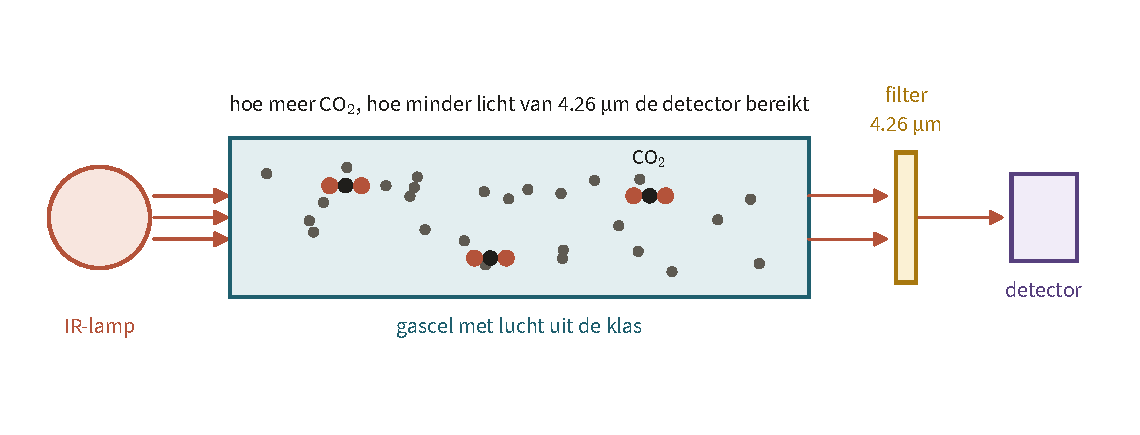
\includegraphics[width=0.85\linewidth]{Figuren/ndir_sensor}
    \caption{Principe van een CO$_2$-meter (niet-dispersieve infraroodsensor). Enkel CO$_2$ absorbeert het licht van \SI{4.26}{\micro\metre}; stikstof, zuurstof en argon, samen meer dan \SI{99.9}{\percent} van de lucht, laten het door.}
    \label{fig:ndir}
\end{figure}

Hetzelfde verschijnsel bepaalt het klimaat. Lucht bestaat voor \SI{78}{\percent} uit stikstof en voor \SI{21}{\percent} uit zuurstof, maar die gassen laten infrarood licht ongehinderd door. Het zijn sporengassen, vooral waterdamp en CO$_2$, die de warmtestraling van de aarde tegenhouden. Zonder hen zou de gemiddelde temperatuur aan het aardoppervlak ongeveer \SI{-18}{\celsius} zijn in plaats van \SI{15}{\celsius}.

Wie dit wil begrijpen, botst op vragen die de thermodynamica van hoofdstuk~\ref{ch:energie} niet kan beantwoorden:
\begin{itemize}
\item De zon straalt vooral zichtbaar licht uit, de aarde infrarood. Waar komt dat verschil vandaan, en wat kan elk soort straling met een molecule doen (\S\ref{sec:licht-pakketjes})?
\item Waarom absorbeert een gas enkel bij welbepaalde golflengten, zoals \SI{4.26}{\micro\metre}, en niet ertussen (\S\ref{sec:lijnenspectra})?
\item Stikstof is het hoofdbestanddeel van de lucht, en toch reageert het bijna nergens mee. Waarom is die molecule zo stabiel (\S\ref{sec:molecuulorbitalen})?
\item Waarom absorbeert CO$_2$ infrarood en stikstof niet, hoewel beide moleculen trillen (\S\ref{sec:moleculaire-beweging})?
\item Waarom heeft CO$_2$ een veel grotere warmtecapaciteit dan stikstof, en waarom stijgt die met de temperatuur (\S\ref{sec:kwantum-thermo})?
\end{itemize}
De antwoorden liggen op de schaal van atomen en moleculen. Daar blijkt energie niet continu maar \emph{gekwantiseerd}: enkel bepaalde waarden zijn toegelaten. Dat geldt voor de elektronen in een atoom, wat de chemische binding en de reactie-enthalpie verklaart, en voor de rotatie en de trilling van een molecule als geheel, wat de absorptie van infrarood en de warmtecapaciteit verklaart.

Net als in hoofdstuk~\ref{ch:energie} start elke sectie met een concreet probleem, bouwt ze de theorie op die nodig is om het op te lossen, en werkt ze het probleem op het einde uit. Het doel is geen volledige cursus kwantummechanica, maar de fundamenten die later terugkomen: de elektronenstructuur bepaalt hoe sterk een molecule aan een katalysator bindt (hoofdstuk~\ref{ch:grensvlakken}), de verdeling van moleculen over hun energieniveaus leidt naar de entropie (hoofdstuk~\ref{ch:spontaniteit}), en vibratie- en rotatieniveaus zijn de basis van de spectroscopie die je in latere vakken gebruikt.

\section{Licht komt in pakketjes}
\label{sec:licht-pakketjes}

\begin{casus}{zon en aarde}
De zon straalt vooral zichtbaar licht uit, de aarde vooral infrarood. We zoeken in deze sectie drie dingen:
\begin{enumerate}
\item bij welke golflengte de zon en de aarde het meest uitstralen, en waarom die zo verschillen;
\item hoeveel energie één foton van elk soort straling draagt, vergeleken met de energie van een chemische binding;
\item hoe warm de aarde zou zijn als haar atmosfeer geen infrarood tegenhield.
\end{enumerate}
\emph{Gegevens.} Het oppervlak van de zon is ongeveer \SI{5800}{\kelvin}, het aardoppervlak gemiddeld \SI{15}{\celsius} (\SI{288}{\kelvin}). Bij de aarde levert de zon \SI{1361}{\watt\per\metre\squared} op een vlak loodrecht op de stralen (de \emph{zonneconstante} $S$). De aarde weerkaatst \SI{30}{\percent} van dat licht. Een C--C-binding heeft een bindingsenergie van \SI{348}{\kilo\joule\per\mole}.

\emph{Schat eerst zelf:} heeft een foton zichtbaar licht meer of minder energie dan een foton infrarood? Kan zonlicht een binding breken? En zou de aarde zonder broeikasgassen warmer of kouder zijn dan nu, en ongeveer hoeveel?
\end{casus}

Rond 1900 leek de natuurkunde bijna af. De wetten van Newton, de thermodynamica en de elektromagnetische theorie van Maxwell verklaarden een enorm gebied aan verschijnselen. Toch bleven enkele waarnemingen onverklaarbaar. Volgens de klassieke fysica kan een atoom zelfs niet stabiel zijn: een elektron dat rond een kern draait, is een versnelde lading, zendt dus straling uit, verliest energie en zou binnen een fractie van een seconde al spiralerend in de kern storten. Drie experimenten toonden waar het misliep: de straling van een gloeiend voorwerp, het foto-elektrisch effect en de lijnenspectra van atomen. We bekijken ze een voor een. De klassieke fysica blijkt daarbij niet fout, maar een benadering die enkel voor grote voorwerpen geldt.

\subsection{Energie als discrete grootheid}

\paragraph{Het probleem: de kleur van een gloeiend voorwerp.}
Een metalen staaf die je verwarmt, gloeit eerst donkerrood, dan oranje, geel en uiteindelijk bijna wit. De kleur van het uitgezonden licht hangt dus rechtstreeks af van de temperatuur. Om dat te begrijpen, bestudeerden natuurkundigen een geïdealiseerd voorwerp dat alle invallende straling absorbeert en ze bij zijn eigen temperatuur weer uitzendt: een \emph{zwart lichaam}. In het labo maak je er een met een holle oven met een klein gaatje in de wand (figuur~\ref{fig:trillingsmodi}a). Licht dat door het gaatje binnenvalt, weerkaatst zo vaak op de wanden dat het nooit meer buitenkomt; wat uit het gaatje straalt, is zuiver de warmtestraling van de wanden. Het spectrum van die straling kon men rond 1900 zeer nauwkeurig meten. Het werd de toetssteen voor elke theorie.

\paragraph{Wat is een trillingsmodus?}
In de holte vormt het elektromagnetische veld golven die heen en weer weerkaatsen tussen de wanden. Een golf kan daar niet om het even hoe trillen. Net als een gitaarsnaar die aan beide uiteinden vastzit, moet de golf aan een geleidende wand nul zijn. Er passen dus enkel \emph{staande golven} met een geheel aantal halve golflengten tussen de wanden: $L = n\lambda/2$, met $n = 1, 2, 3, \ldots$ Elk zo'n toegelaten trillingspatroon heet een \emph{trillingsmodus} van het stralingsveld. Een modus is dus geen deeltje en geen atoom, maar een manier waarop het veld in de holte kan trillen, met een eigen golflengte en frequentie.

Hoe korter de golflengte, hoe meer manieren er zijn om een staande golf in de holte te passen. Op een snaar zie je dat al: tussen golflengte $2L$ en $L$ ligt één modus, maar tussen $2L/10$ en $L/10$ liggen er tien. In drie dimensies kan de golf bovendien in alle richtingen staan, en stijgt het aantal modi per frequentie-interval met $\nu^2$. Er zijn dus veel meer modi bij hoge dan bij lage frequenties.

\begin{figure}[htb]
    \centering
    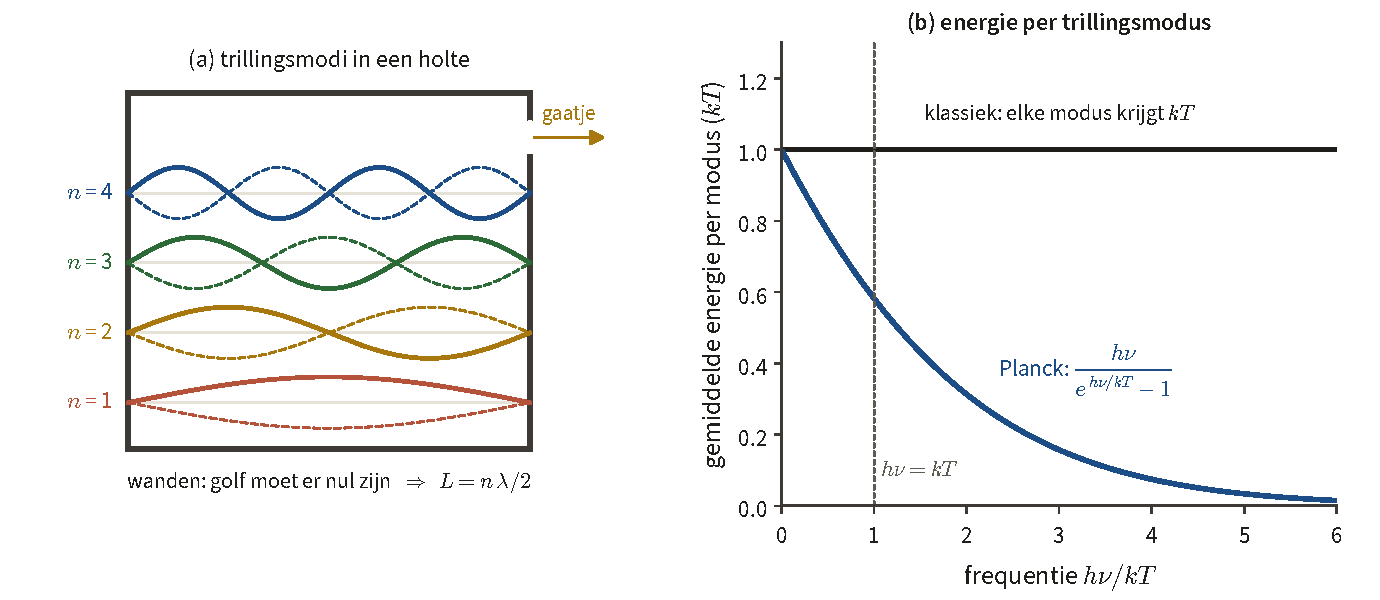
\includegraphics[width=0.95\linewidth]{Figuren/trillingsmodi}
    \caption{(a) Een zwart lichaam als holte met een gaatje. Tussen de wanden passen enkel staande golven met een geheel aantal halve golflengten: de trillingsmodi. (b) De gemiddelde energie per modus. Klassiek krijgt elke modus $kT$; volgens Planck daalt die energie sterk zodra $h\nu$ groter wordt dan $kT$.}
    \label{fig:trillingsmodi}
\end{figure}

\paragraph{De ultravioletcatastrofe.}
De klassieke statistische fysica kent aan elke trillingsmodus gemiddeld dezelfde energie $kT$ toe, net zoals ze dat doet voor elke vrijheidsgraad van een gasmolecule (de \emph{equipartitiestelling}). Het uitgestraalde vermogen bij een frequentie is dan evenredig met het aantal modi maal $kT$, dus met $\nu^2 kT$. Dat is de wet van Rayleigh en Jeans. Ze werkt goed bij lange golflengten, maar bij hoge frequenties stijgt ze zonder grens. Tel je alle modi op, dan zou een warm voorwerp een \emph{oneindige} hoeveelheid energie uitstralen, vooral in het ultraviolet. Dit werd de \emph{ultravioletcatastrofe} genoemd (figuur~\ref{fig:UVcatastrophe}). De metingen tonen het tegendeel: na een maximum daalt de intensiteit bij hoge frequenties sterk.

\begin{figure}[htb]
    \centering
    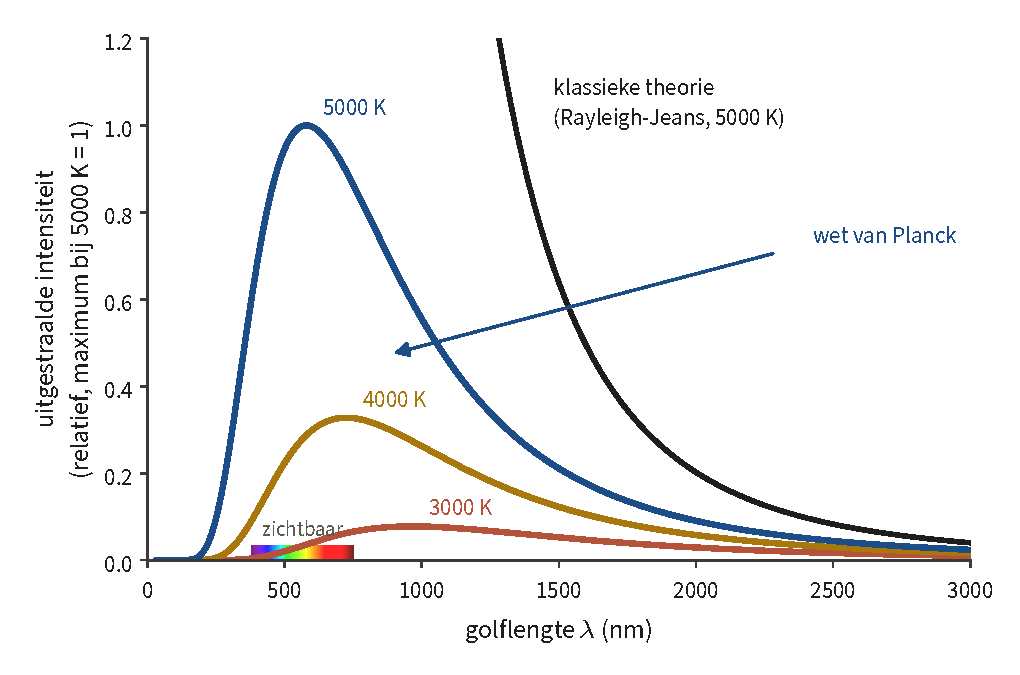
\includegraphics[width=0.62\linewidth]{Figuren/uv_catastrofe}
    \caption{Stralingsspectrum van een zwart lichaam. De wet van Rayleigh--Jeans (klassiek) loopt bij korte golflengten naar oneindig; de wet van Planck volgt de metingen.}
    \label{fig:UVcatastrophe}
\end{figure}

\paragraph{De oplossing van Planck.}
Max Planck loste dit in 1900 op met een gedurfde hypothese: een trillingsmodus met frequentie $\nu$ kan geen willekeurige hoeveelheid energie bevatten, maar enkel een geheel aantal ondeelbare pakketjes, \emph{kwanta}, van grootte
\begin{equation}
\boxed{
E=h\nu=h\frac{c}{\lambda}
}
\end{equation}
met $h=\SI{6.626e-34}{\joule\second}$ de constante van Planck, $\nu$ de frequentie, $\lambda$ de golflengte en $c$ de lichtsnelheid. Een modus bevat dus $0$, $h\nu$, $2h\nu$, \ldots, maar nooit $0.4\,h\nu$.

Waarom lost dat het probleem op? Bij temperatuur $T$ is de typische thermische energie die beschikbaar is van de orde $kT$. Voor een modus met lage frequentie is $h\nu \ll kT$: de pakketjes zijn klein, de energie lijkt continu, en de modus krijgt zoals klassiek ongeveer $kT$. Voor een modus met hoge frequentie is $h\nu \gg kT$: zelfs één pakketje is al te groot om met de beschikbare thermische energie te leveren, en de modus blijft meestal leeg. Planck vond dat de gemiddelde energie per modus gelijk is aan $h\nu/(e^{h\nu/kT}-1)$ (figuur~\ref{fig:trillingsmodi}b). Die uitdrukking volgt uit de Boltzmannverdeling, die we in \S\ref{sec:kwantum-thermo} uitwerken. Vermenigvuldig je ze met het aantal modi, dan krijg je het uitgestraalde vermogen per oppervlakte en per golflengte-interval, de \emph{wet van Planck}:
\begin{equation}
M_\lambda(T) = \frac{2\pi h c^2}{\lambda^5}\,\frac{1}{e^{hc/(\lambda k T)}-1}.
\label{eq:planck}
\end{equation}
Die formule beschrijft het gemeten spectrum bij elke temperatuur. Planck zag zijn kwanta aanvankelijk als een rekentruc, maar ze bleken een fundamentele eigenschap van de natuur. Op macroscopische schaal zijn de kwanta zo klein dat energie continu \emph{lijkt}; op atomaire schaal bepalen ze het gedrag van materie.

\paragraph{Twee gevolgen: de wetten van Wien en van Stefan--Boltzmann.}
Wat betekent de wet van Planck voor de gloeiende staaf? Figuur~\ref{fig:gloeiende-staaf}a toont het spectrum bij \SI{1000}{}, \SI{1250}{} en \SI{1500}{\kelvin}. Twee zaken vallen op, en elk ervan is een wet die je in de techniek voortdurend gebruikt.

\begin{figure}[htb]
    \centering
    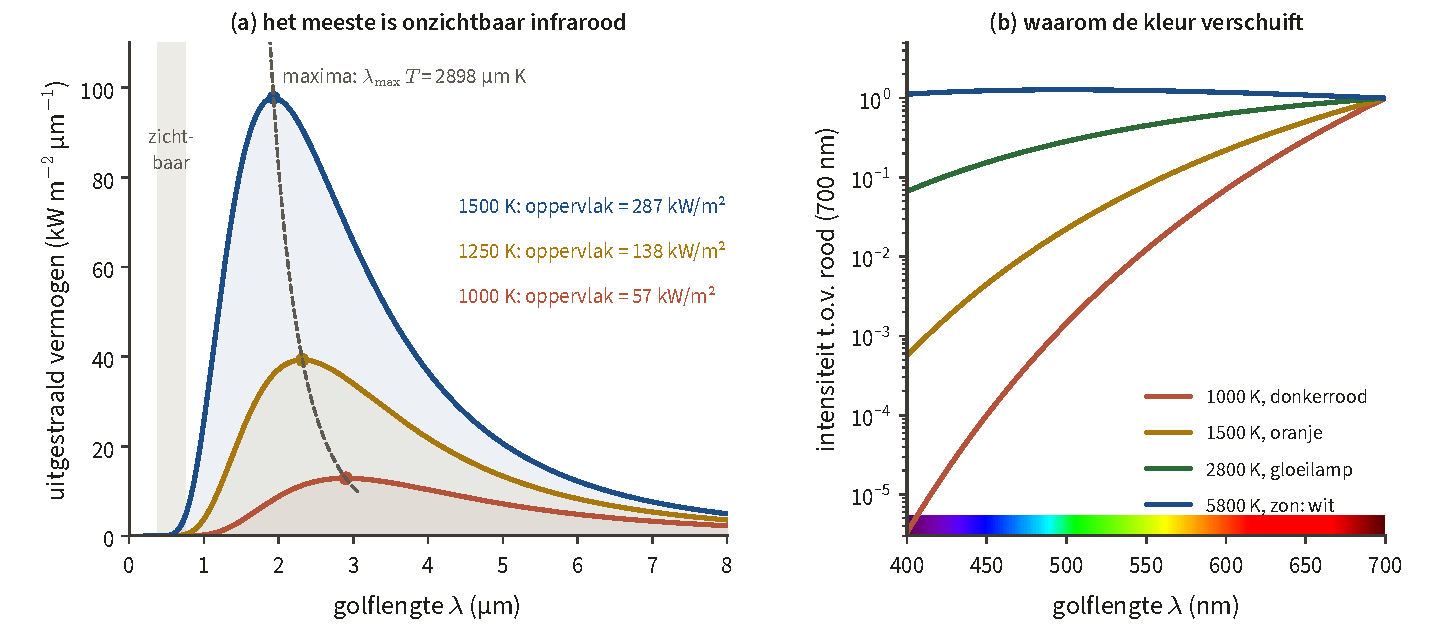
\includegraphics[width=\linewidth]{Figuren/gloeiende_staaf}
    \caption{(a) Straling van een gloeiende staaf volgens de wet van Planck. Het maximum schuift naar kortere golflengten als de temperatuur stijgt (wet van Wien, stippellijn), en het oppervlak onder de kromme, het totale vermogen, stijgt met $T^4$ (wet van Stefan--Boltzmann). Bijna alle straling is onzichtbaar infrarood. (b) Het zichtbare deel, relatief ten opzichte van rood licht. Bij \SI{1000}{\kelvin} is blauw honderdduizend keer zwakker dan rood: de staaf gloeit donkerrood. Bij hogere temperatuur wordt het spectrum in het zichtbare vlakker en het licht witter.}
    \label{fig:gloeiende-staaf}
\end{figure}

Ten eerste schuift het maximum naar kortere golflengten naarmate het voorwerp warmer is. Zoek je het maximum van~\eqref{eq:planck} door de afgeleide naar $\lambda$ nul te stellen, dan vind je dat het product van de golflengte van het maximum en de temperatuur een constante is, de \emph{verschuivingswet van Wien}:
\begin{equation}
\lambda_{\max}\,T = \SI{2898}{\micro\metre\kelvin}.
\label{eq:wien}
\end{equation}
De betekenis is eenvoudig: \emph{de kleur van de straling is een thermometer}. Voor de staaf bij \SI{1000}{\kelvin} ligt het maximum bij \SI{2.9}{\micro\metre}, ver in het infrarood. Slechts een miljoenste van de straling valt in het zichtbare gebied, en dat is het uiterste rode staartje van het spectrum: de staaf gloeit donkerrood, maar vooral voel je zijn warmte. Wordt de staaf warmer, dan schuift de hele kromme naar links, en komt er naast rood steeds meer oranje, geel en blauw licht bij (figuur~\ref{fig:gloeiende-staaf}b). Bij ongeveer \SI{2800}{\kelvin}, de gloeidraad van een klassieke gloeilamp, is het licht bijna wit, maar ligt het maximum nog steeds in het infrarood (\SI{1.0}{\micro\metre}): slechts ongeveer \SI{8}{\percent} van het vermogen is zichtbaar licht. Daarom zijn gloeilampen vervangen door ledlampen.

Ten tweede wordt het oppervlak onder de kromme veel groter. Dat oppervlak is het totale uitgestraalde vermogen per oppervlakte. Integreer je~\eqref{eq:planck} over alle golflengten, dan vind je de \emph{wet van Stefan--Boltzmann}:
\begin{equation}
\frac{P}{A} = \sigma T^4, \qquad \sigma = \SI{5.67e-8}{\watt\per\metre\squared\per\kelvin\tothe{4}}.
\label{eq:stefan-boltzmann}
\end{equation}
Ook hier is de betekenis direct bruikbaar: \emph{het stralingsverlies stijgt met de vierde macht van de temperatuur}. Van \SI{1000}{} naar \SI{1500}{\kelvin} stijgt de temperatuur met de helft, maar de uitstraling met een factor $1.5^4 = 5.1$. Bij kamertemperatuur is straling een bescheiden vorm van warmteoverdracht; in een oven of in de vuurhaard van een stoomketel is ze dominant. Een echt oppervlak straalt minder dan een zwart lichaam, $P/A = \varepsilon\sigma T^4$, met een \emph{emissiviteit} $\varepsilon$ tussen 0 en 1: ongeveer 0.05 voor blank gepolijst metaal, 0.8 tot 0.9 voor geoxideerd staal, baksteen en de menselijke huid.

Beide wetten gebruik je meer dan je denkt. Een thermische camera of oorthermometer meet het infrarood rond \SI{10}{\micro\metre}: volgens~\eqref{eq:wien} straalt een mens van \SI{310}{\kelvin} het sterkst bij \SI{9.3}{\micro\metre}. Een pyrometer meet de temperatuur van gesmolten staal of van een ovenwand zonder contact, uit de intensiteit of de kleur van de straling. En de isolatie van ovens en stoomleidingen wordt berekend met~\eqref{eq:stefan-boltzmann}.

\begin{voorbeeld}{Hoeveel straalt een gloeiende staaf uit?}
Een stalen staaf met diameter \SI{2.0}{\centi\metre} en lengte \SI{30}{\centi\metre} ($\varepsilon = 0.80$) wordt in een smidse verhit tot \SI{1000}{\kelvin}. Het zijoppervlak is $A = \pi d L = \pi(0.020)(0.30) = \SI{0.0188}{\metre\squared}$. De staaf straalt
\[
P = \varepsilon\sigma T^4 A = (0.80)(5.67\times10^{-8})(1000)^4(0.0188) = \SI{855}{\watt}
\]
uit, ongeveer evenveel als een waterkoker op halve kracht. De omgeving van \SI{300}{\kelvin} straalt terug met $(300/1000)^4 = \SI{0.8}{\percent}$ daarvan, wat verwaarloosbaar is. Bij \SI{1500}{\kelvin} wordt dat $855 \times 5.06 = \SI{4.3}{\kilo\watt}$. Om een staaf op hoge temperatuur te houden, moet de smid dus steeds sneller warmte toevoeren.
\end{voorbeeld}

\begin{figure}[htb]
    \centering
    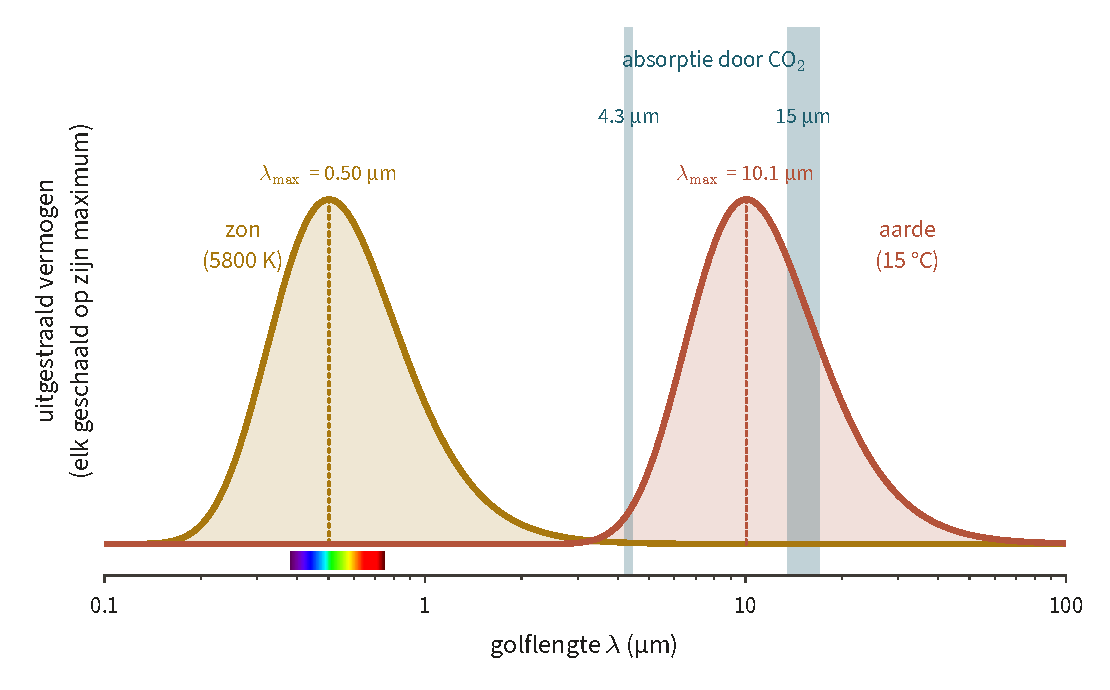
\includegraphics[width=0.8\linewidth]{Figuren/zon_aarde_spectrum}
    \caption{Straling van de zon (oppervlak \SI{5800}{\kelvin}) en van de aarde (\SI{15}{\celsius}) volgens de wet van Planck, elk geschaald op zijn maximum. De twee spectra overlappen nauwelijks. De gekleurde banden zijn de sterkste absorptiebanden van CO$_2$: ze vallen in het infrarood van de aarde, niet in het zonlicht.}
    \label{fig:zon-aarde}
\end{figure}

\paragraph{De energie van één foton.}
Om een gevoel te krijgen voor de grootte van $E=h\nu$, vergelijken we drie soorten straling.

\begin{voorbeeld}{Fotonenergie over het elektromagnetisch spectrum}
Met $E=hc/\lambda$ en $c=\SI{3.00e8}{\meter\per\second}$:
\begin{align*}
E_{\text{radio}} &= \frac{(6.626\times10^{-34})(3.00\times10^{8})}{3} = \SI{6.63e-26}{\joule} \quad (\lambda=\SI{3}{\meter}) \\
E_{\text{groen}} &= \frac{(6.626\times10^{-34})(3.00\times10^{8})}{520\times10^{-9}} = \SI{3.82e-19}{\joule} \quad (\lambda=\SI{520}{\nano\meter}) \\
E_{\text{X}} &= \frac{(6.626\times10^{-34})(3.00\times10^{8})}{0.1\times10^{-9}} = \SI{1.99e-15}{\joule} \quad (\lambda=\SI{0.1}{\nano\meter})
\end{align*}
Tussen radio en röntgen zit een factor $10^{10}$, hoewel beide ``gewoon'' elektromagnetische straling zijn. Radiogolven zijn daarom onschadelijk voor chemische bindingen, terwijl UV- en röntgenfotonen bindingen kunnen breken of elektronen kunnen losmaken: hun energie ligt in dezelfde grootteorde als elektronische energieverschillen (figuur~\ref{fig:spectrum-bindingen}).
\end{voorbeeld}

\begin{figure}[htb]
    \centering
    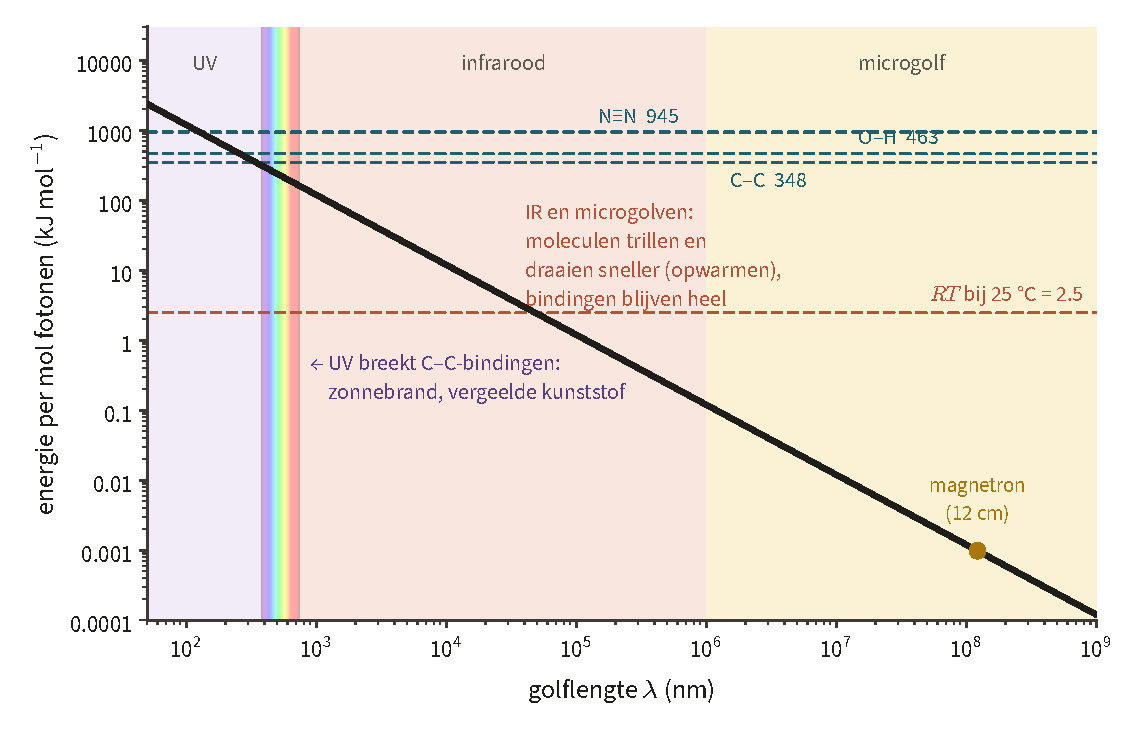
\includegraphics[width=0.62\linewidth]{Figuren/spectrum_bindingen}
    \caption{Energie van één mol fotonen over het elektromagnetisch spectrum, vergeleken met enkele bindingsenergieën en met $RT$ bij kamertemperatuur. Ultraviolet licht kan C--C-bindingen breken (zonnebrand, vergeelde kunststof); infrarood en microgolven doen moleculen enkel sneller trillen en draaien.}
    \label{fig:spectrum-bindingen}
\end{figure}

\subsection{Het foto-elektrisch effect}

\paragraph{Het experiment.}
Planck had de kwanta ingevoerd voor de uitwisseling van energie tussen materie en straling. Of het licht zelf uit pakketjes bestaat, bleef open. Het antwoord kwam uit een experiment dat Heinrich Hertz in 1887 bij toeval opmerkte: een vonk sprong gemakkelijker over wanneer de elektroden met ultraviolet licht werden beschenen. Philipp Lenard onderzocht het effect rond 1902 systematisch met de opstelling van figuur~\ref{fig:foto-opstelling}a. In een vacuümbuis staan twee elektroden: een metalen plaat en een collector. Licht valt door een kwartsvenster, dat ook UV doorlaat, op de plaat. Maakt het licht elektronen vrij, dan vliegen sommige naar de collector en meet een ampèremeter in de uitwendige kring een stroom.

Met een regelbare spanning kun je de collector ook negatief maken ten opzichte van de plaat. Die \emph{tegenspanning} $U$ remt de elektronen af: enkel elektronen met een kinetische energie groter dan $eU$ bereiken de collector nog. Bij een bepaalde \emph{stopspanning} $U_s$ valt de stroom volledig weg. Ook het snelste elektron haalt de collector dan net niet, zodat
\[
E_{\mathrm{kin,max}} = eU_s .
\]
Zo meet je met een eenvoudige voltmeter de maximale energie van de vrijgemaakte elektronen. Lenard varieerde vervolgens de intensiteit en de frequentie (de kleur) van het licht.

\begin{figure}[htb]
    \centering
    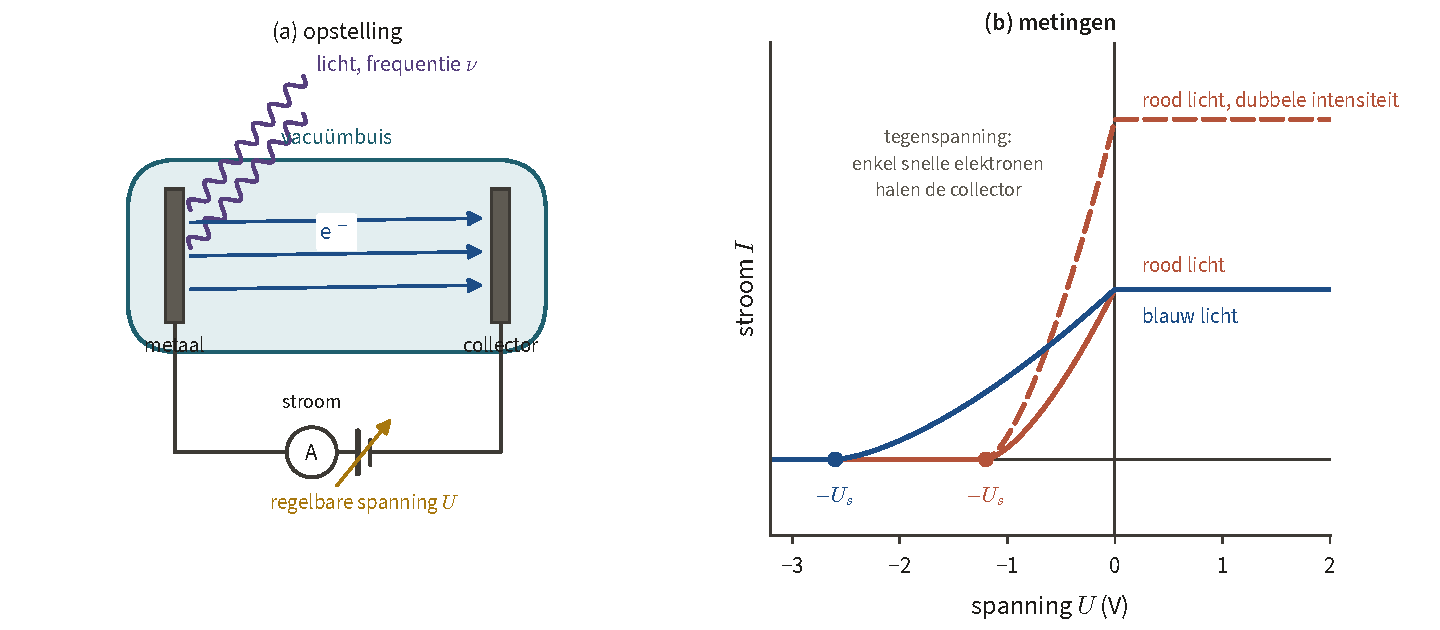
\includegraphics[width=\linewidth]{Figuren/foto_opstelling}
    \caption{(a) Opstelling voor het foto-elektrisch effect. Licht maakt elektronen vrij uit een metalen plaat; met een tegenspanning $U$ wordt gemeten hoe snel ze zijn. (b) Stroom tegen spanning. Dubbel zoveel licht van dezelfde kleur geeft een dubbele stroom, maar dezelfde stopspanning $U_s$. Licht met een hogere frequentie geeft een grotere stopspanning, dus snellere elektronen.}
    \label{fig:foto-opstelling}
\end{figure}

\paragraph{De waarnemingen.}
Volgens de klassieke golftheorie draagt een lichtgolf haar energie continu, evenredig met haar intensiteit. Intenser licht zou de elektronen dus sneller moeten maken, en bij zwak licht zou het even moeten duren voor een elektron genoeg energie heeft opgestapeld. De metingen (figuur~\ref{fig:foto-opstelling}b) toonden iets heel anders:
\begin{enumerate}
\item Onder een \emph{drempelfrequentie} $\nu_0$ komt geen enkel elektron vrij, hoe intens het licht ook is. Rood licht maakt uit zink geen elektronen vrij, ook niet met een sterke lamp; zwak UV-licht doet dat wel.
\item Boven de drempel komen de elektronen \emph{onmiddellijk} vrij, ook bij zeer zwak licht. Er is geen opstapeltijd.
\item Meer licht van dezelfde kleur geeft \emph{meer} elektronen (een grotere stroom), maar niet \emph{snellere}: de stopspanning blijft dezelfde. De maximale kinetische energie hangt enkel af van de frequentie.
\end{enumerate}

\paragraph{De verklaring van Einstein.}
In 1905 stelde Einstein dat licht zelf uit energiepakketjes bestaat, later \emph{fotonen} genoemd, elk met energie $h\nu$. Eén elektron absorbeert telkens één volledig foton. Een deel van die energie, de \emph{werkfunctie} $\Phi$, is nodig om het elektron uit het metaal te halen; de rest wordt kinetische energie (figuur~\ref{fig:photoelectric}):
\begin{equation}
h\nu = \Phi + E_{\mathrm{kin,max}}
\qquad\text{of}\qquad
\boxed{E_{\mathrm{kin,max}} = \tfrac{1}{2}m_ev^2 = h\nu-\Phi .}
\end{equation}
De drie waarnemingen volgen er meteen uit. Is $h\nu < \Phi$, dan kan geen enkel foton een elektron vrijmaken, hoeveel fotonen er ook zijn (waarneming 1). Is $h\nu > \Phi$, dan gebeurt het bij de eerste absorptie (waarneming 2). Intenser licht betekent meer fotonen, dus meer elektronen, maar elk foton heeft nog steeds dezelfde energie (waarneming 3). De drempelfrequentie is $\nu_0 = \Phi/h$.

\begin{figure}[htb]
    \centering
    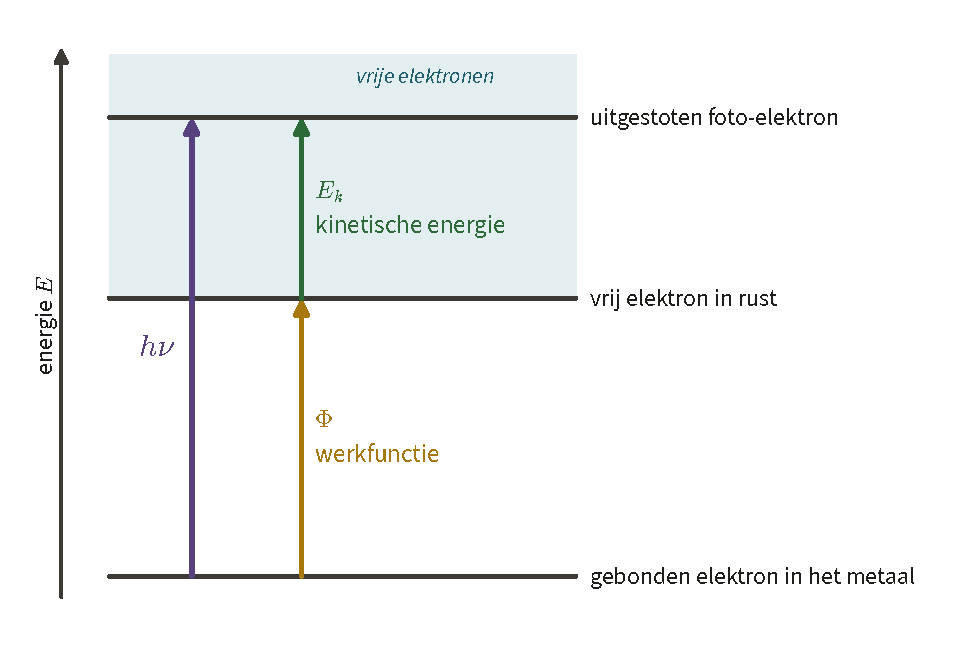
\includegraphics[width=0.55\linewidth]{Figuren/foto_elektrisch}
    \caption{Een foton met energie $h\nu$ maakt een elektron vrij: een deel van de energie dient om het metaal te verlaten ($\Phi$), de rest wordt kinetische energie ($E_k$).}
    \label{fig:photoelectric}
\end{figure}

Robert Millikan, die Einstein aanvankelijk wilde weerleggen, mat in 1916 de stopspanning bij veel frequenties en voor verschillende metalen. Hij vond rechte lijnen met voor elk metaal dezelfde helling $h$ (figuur~\ref{fig:ek-frequentie}), en bepaalde zo de constante van Planck tot op een half procent nauwkeurig.

\begin{figure}[htb]
    \centering
    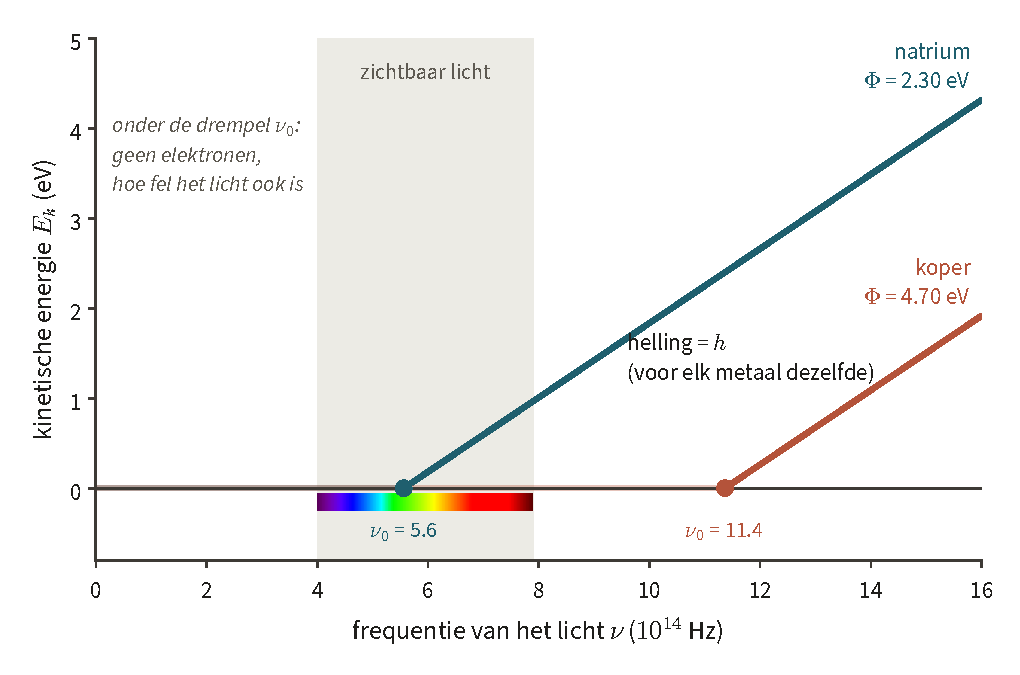
\includegraphics[width=0.6\linewidth]{Figuren/ek_frequentie}
    \caption{Maximale kinetische energie van de uitgestoten elektronen tegen de frequentie, voor natrium en koper. Onder $\nu_0 = \Phi/h$ komen geen elektronen vrij; daarboven stijgt $E_{\mathrm{kin,max}}$ lineair met helling $h$, voor elk metaal dezelfde.}
    \label{fig:ek-frequentie}
\end{figure}

Energieën op deze schaal druk je handig uit in \emph{elektronvolt}: $\SI{1}{\electronvolt}=\SI{1.602e-19}{\joule}$ is de energie die één elektron krijgt bij een spanningsverschil van \SI{1}{\volt}. Een stopspanning van \SI{2.66}{\volt} betekent dus een maximale kinetische energie van \SI{2.66}{\electronvolt}. Typische werkfuncties liggen tussen \SI{2}{} en \SI{5}{\electronvolt}.

\begin{voorbeeld}{Foto-elektrisch effect}
Natrium ($\Phi=\SI{2.30}{eV}$) wordt bestraald met UV-licht van \SI{250}{nm}. Eén foton heeft
\[
E=\frac{hc}{\lambda}=\frac{(6.626\times10^{-34})(3.00\times10^{8})}{250\times10^{-9}}=\SI{7.95e-19}{J}=\SI{4.96}{eV},
\]
zodat $E_{\mathrm{kin,max}}=4.96-2.30=\SI{2.66}{eV}$. In de opstelling van figuur~\ref{fig:foto-opstelling} is een tegenspanning van \SI{2.66}{\volt} nodig om de stroom te stoppen. De drempelgolflengte van natrium is $\lambda_0 = hc/\Phi = \SI{539}{\nano\metre}$: groen licht maakt nog net elektronen vrij, rood licht niet.
\end{voorbeeld}

De werkfunctie mag je niet verwarren met de ionisatie-energie. De werkfunctie is de energie om een elektron uit een vast metaal te halen; dat elektron bewoog al vrij door het metaal en moet enkel het oppervlak verlaten. De ionisatie-energie is de energie om een elektron volledig los te maken van één vrij atoom, tegen de volle aantrekking van de kern in. Voor natrium is de werkfunctie \SI{2.3}{\electronvolt}, de eerste ionisatie-energie \SI{5.1}{\electronvolt}.

Het foto-elektrisch effect is ook technisch belangrijk. Een fotocel of lichtsensor werkt op dit principe, en een zonnecel is er een variant van: daar wordt het elektron niet uit het materiaal gestoten, maar naar een hogere energieband gebracht, waar het als stroom kan wegvloeien. Ook dan geldt de drempel: silicium reageert enkel op fotonen boven ongeveer \SI{1.1}{\electronvolt}, dus golflengten korter dan \SI{1.1}{\micro\metre}.

\begin{casusuitgewerkt}{zon en aarde}
\emph{Stap 1: waar stralen zon en aarde het meest?} Met de wet van Wien~\eqref{eq:wien}:
\[
\lambda_{\max,\text{zon}} = \frac{\SI{2898}{\micro\metre\kelvin}}{\SI{5800}{\kelvin}} = \SI{0.50}{\micro\metre}, \qquad
\lambda_{\max,\text{aarde}} = \frac{\SI{2898}{\micro\metre\kelvin}}{\SI{288}{\kelvin}} = \SI{10.1}{\micro\metre}.
\]
De zon straalt het meest in het groen, de aarde in het verre infrarood (figuur~\ref{fig:zon-aarde}). Het verschil komt enkel van de temperatuur: zon en aarde zijn allebei, bij benadering, zwarte lichamen.

Waarom \SI{5800}{\kelvin}? De zon heeft geen vast oppervlak. Het licht dat ons bereikt, ontsnapt uit een laag van enkele honderden kilometer dik, de \emph{fotosfeer}, en die heeft ongeveer \SI{5800}{\kelvin}. Dieper in de zon is het veel heter (in de kern ongeveer 15~miljoen kelvin), en de ijle corona erboven haalt zelfs 1 tot 2~miljoen kelvin, maar straalt door haar lage dichtheid nauwelijks. Je kunt de \SI{5800}{\kelvin} zelf controleren met de wet van Stefan--Boltzmann. De zon straalt in totaal \SI{3.83e26}{\watt} uit over een bol met straal \SI{6.96e8}{\metre}:
\[
T = \left(\frac{P}{4\pi R^2\sigma}\right)^{1/4} = \left(\frac{3.83\times10^{26}}{4\pi(6.96\times10^{8})^2(5.67\times10^{-8})}\right)^{1/4} = \SI{5770}{\kelvin}.
\]

\emph{Stap 2: de energie per foton.} Per mol fotonen is $E_\mathrm{m} = N_\mathrm{A}hc/\lambda$:
\[
E_\mathrm{m}(\SI{0.50}{\micro\metre}) = \SI{239}{\kilo\joule\per\mole}, \qquad
E_\mathrm{m}(\SI{10}{\micro\metre}) = \SI{12}{\kilo\joule\per\mole}.
\]
Zichtbaar licht komt in de buurt van bindingsenergieën; UV-licht ($\lambda < \SI{0.35}{\micro\metre}$, meer dan \SI{340}{\kilo\joule\per\mole}) gaat erover en kan C--C-bindingen breken. Een infraroodfoton van de aarde heeft dertig keer te weinig energie om een binding te breken. Het kan een molecule enkel sneller laten trillen of draaien (figuur~\ref{fig:spectrum-bindingen}).

\emph{Stap 3: hoe koud zou de aarde zijn zonder broeikasgassen?} We stellen een energiebalans op voor de aarde als geheel (figuur~\ref{fig:stralingsbalans}). In evenwicht is wat binnenkomt gelijk aan wat buitengaat.
\begin{itemize}
\item \emph{In.} De zonnestralen vallen evenwijdig in. De aarde onderschept er evenveel van als een platte schijf met dezelfde straal: haar schaduw is een cirkel met oppervlak $\pi r^2$. Daarvan wordt \SI{30}{\percent} weerkaatst door wolken, ijs en woestijnen. Er wordt dus $(1-0.30)\,S\,\pi r^2$ geabsorbeerd.
\item \emph{Uit.} De aarde draait en houdt haar warmte vast, zodat ze dag en nacht en over haar volledige boloppervlak $4\pi r^2$ infrarood uitstraalt: $\sigma T^4 \cdot 4\pi r^2$.
\end{itemize}
Gelijkstellen geeft
\[
\sigma T^4 \cdot 4\pi r^2 = (1-0.30)\,S\,\pi r^2
\quad\Longrightarrow\quad
\sigma T^4 = \frac{(1-0.30)(1361)}{4} = \SI{238}{\watt\per\metre\squared}.
\]
De straal van de aarde valt weg; de factor 4 is de verhouding tussen het oppervlak van een bol en dat van zijn schaduw. Dan is
\[
T = \left(\frac{238}{5.67\times10^{-8}}\right)^{1/4} = \SI{255}{\kelvin} = \SI{-18}{\celsius}.
\]
De werkelijke gemiddelde temperatuur is \SI{15}{\celsius}. Het verschil van \SI{33}{\kelvin} is het natuurlijke broeikaseffect: een deel van het infrarood van de aarde wordt in de atmosfeer geabsorbeerd en gedeeltelijk teruggestraald naar het oppervlak, dat daardoor warmer moet worden om evenveel kwijt te raken.

\emph{Volgende vraag.} Figuur~\ref{fig:zon-aarde} toont dat CO$_2$ niet het hele infrarood absorbeert, maar enkel smalle banden rond \SI{4.3}{} en \SI{15}{\micro\metre}. Waarom absorbeert een gas enkel bij welbepaalde golflengten?
\end{casusuitgewerkt}

\begin{figure}[htb]
    \centering
    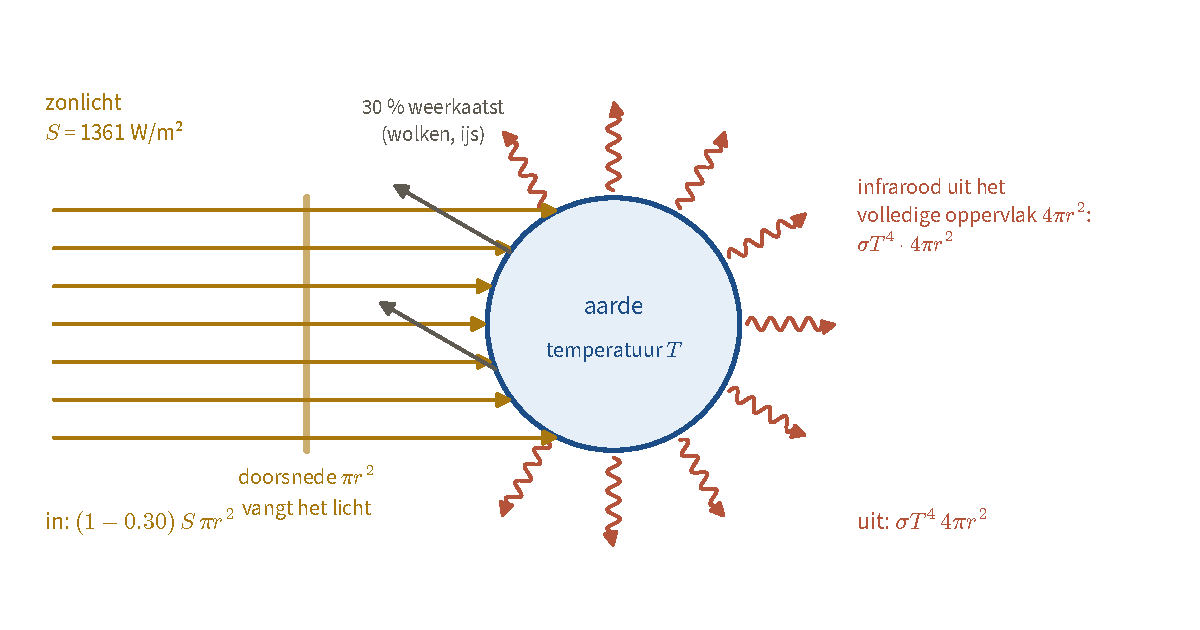
\includegraphics[width=0.85\linewidth]{Figuren/stralingsbalans_aarde}
    \caption{Stralingsbalans van de aarde. Het zonlicht wordt opgevangen door de doorsnede $\pi r^2$; \SI{30}{\percent} wordt weerkaatst. De aarde straalt infrarood uit over haar volledige oppervlak $4\pi r^2$.}
    \label{fig:stralingsbalans}
\end{figure}

\section{Discrete energieniveaus en lijnenspectra}
\label{sec:lijnenspectra}

\begin{casus}{scherpe lijnen}
De CO$_2$-meter van figuur~\ref{fig:ndir} gebruikt een filter van \SI{4.26}{\micro\metre}. Bij \SI{4.0}{} of \SI{4.6}{\micro\metre} zou hij niets meten: daar absorbeert CO$_2$ niet. Een gas absorbeert dus niet geleidelijk over het hele spectrum, maar bij scherpe golflengten. Hoe kan dat, en welke energie hoort bij \SI{4.26}{\micro\metre}?

\emph{Schat eerst zelf:} als een molecule enkel bepaalde energieën kan hebben, wat betekent dat voor de fotonen die ze kan opnemen?
\end{casus}

\subsection{Het model van Bohr}
\label{sec:bohr}

\paragraph{De waarneming: het lijnenspectrum van waterstof.}
Stuur je een elektrische ontlading door een buis met waterstofgas, dan splitst de ontlading de \ce{H2}-moleculen in atomen en geeft ze die atomen extra energie. De buis licht roze-paars op. Laat je dat licht door een smalle spleet en een prisma of tralie vallen (figuur~\ref{fig:waterstof-opstelling}), dan zie je geen doorlopende regenboog zoals bij een gloeiende staaf, maar slechts vier scherpe gekleurde lijnen: bij \SI{656}{} (rood), \SI{486}{} (blauwgroen), \SI{434}{} en \SI{410}{\nano\metre} (violet). Dit is een \emph{lijnenspectrum}, en elk element heeft er een eigen.

\begin{figure}[htb]
    \centering
    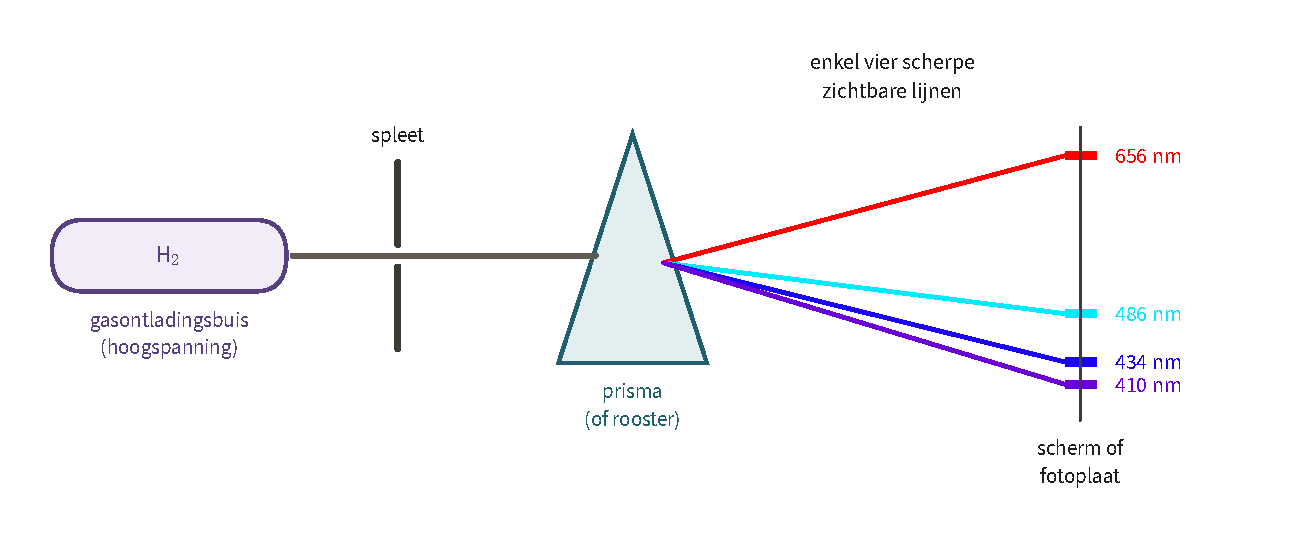
\includegraphics[width=0.9\linewidth]{Figuren/waterstof_opstelling}
    \caption{Het lijnenspectrum van waterstof. Het licht van een gasontladingsbuis wordt na een spleet door een prisma (of tralie) uitgesplitst. Op het scherm verschijnen enkel vier scherpe zichtbare lijnen.}
    \label{fig:waterstof-opstelling}
\end{figure}

In 1885 merkte de Zwitserse leraar Johann Balmer op dat de vier golflengten passen in een eenvoudige formule, $\lambda = B\,n^2/(n^2-4)$ met $B = \SI{364.6}{\nano\metre}$ en $n = 3, 4, 5, 6$. Probeer maar: $n=3$ geeft $364.6 \times 9/5 = \SI{656}{\nano\metre}$. Rydberg schreef dit later om tot
\[
\frac{1}{\lambda} = R_H\left(\frac{1}{2^2} - \frac{1}{n^2}\right), \qquad R_H = \SI{1.097e7}{\per\metre},
\]
en voorspelde dat er ook reeksen met $1/1^2$ en $1/3^2$ moesten bestaan. Die werden later gevonden in het ultraviolet (Lyman) en het infrarood (Paschen). De formule werkte perfect, maar niemand wist waarom. Waarom zendt waterstof enkel deze golflengten uit, en waarom zijn ze te schrijven als een verschil van twee termen $1/n^2$?

\paragraph{De postulaten van Bohr.}
Niels Bohr gaf in 1913 het eerste antwoord. Hij hield het klassieke beeld van een elektron dat op een cirkelbaan rond de kern draait, vastgehouden door de Coulombaantrekking, maar voegde er twee niet-klassieke postulaten aan toe:
\begin{enumerate}
\item Enkel banen waarvoor het impulsmoment een geheel veelvoud is van $\hbar = h/2\pi$ zijn toegelaten:
\begin{equation}
m_e v r = n\hbar, \qquad n=1,2,3,\ldots
\label{eq:bohr-kwantisatie}
\end{equation}
Op zo'n baan straalt het elektron, in strijd met de klassieke fysica, \emph{niet}. Het atoom is daar stabiel.
\item Het atoom zendt enkel straling uit wanneer het elektron van een baan met energie $E_j$ naar een lagere baan $E_i$ springt. Het energieverschil verlaat het atoom als één foton: $h\nu = E_j - E_i$.
\end{enumerate}

\paragraph{De afleiding, stap voor stap.}
Uit deze twee postulaten en de gewone klassieke mechanica volgen de toegelaten banen en energieën.

\emph{Stap 1: krachtevenwicht.} De Coulombkracht tussen kern ($+e$) en elektron ($-e$) levert de centripetale kracht die nodig is om het elektron op een cirkelbaan met straal $r$ te houden:
\[
\frac{e^2}{4\pi\varepsilon_0 r^2} = \frac{m_e v^2}{r}
\qquad\Longrightarrow\qquad
m_e v^2 = \frac{e^2}{4\pi\varepsilon_0 r}.
\]
Klassiek is elke straal $r$ mogelijk, met een bijbehorende snelheid $v$.

\emph{Stap 2: kwantisatie.} Uit~\eqref{eq:bohr-kwantisatie} is $v = n\hbar/(m_e r)$. Invullen in stap~1 geeft
\[
m_e \frac{n^2\hbar^2}{m_e^2 r^2} = \frac{e^2}{4\pi\varepsilon_0 r}
\qquad\Longrightarrow\qquad
r_n = n^2\,\frac{4\pi\varepsilon_0\hbar^2}{m_e e^2} = n^2 a_0 .
\]
Enkel welbepaalde stralen zijn nu toegelaten. De kleinste, voor $n=1$, is de \emph{straal van Bohr}:
\[
a_0 = \frac{4\pi\varepsilon_0\hbar^2}{m_e e^2} = \SI{52.9}{\pico\metre}.
\]
Dat is precies de grootteorde van een atoom. Het elektron beweegt daar met $v = \hbar/(m_e a_0) = \SI{2.19e6}{\metre\per\second}$, ongeveer \SI{0.7}{\percent} van de lichtsnelheid.

\emph{Stap 3: de energie.} De totale energie is de som van de kinetische en de potentiële energie. Met stap~1 is $\tfrac12 m_e v^2 = \tfrac12\, e^2/(4\pi\varepsilon_0 r)$, zodat
\[
E = \tfrac12 m_e v^2 - \frac{e^2}{4\pi\varepsilon_0 r}
= \frac{e^2}{8\pi\varepsilon_0 r} - \frac{e^2}{4\pi\varepsilon_0 r}
= -\frac{e^2}{8\pi\varepsilon_0 r}.
\]
De energie is negatief: het elektron is gebonden, en je moet energie toevoeren om het los te maken. De kinetische energie is precies de helft van de absolute waarde van de potentiële energie.

\emph{Stap 4: de toegelaten energieën.} Vul $r_n = n^2 a_0$ uit stap~2 in:
\begin{equation}
\boxed{
E_n = -\frac{e^2}{8\pi\varepsilon_0 a_0}\,\frac{1}{n^2} = -\frac{m_e e^4}{8\varepsilon_0^2 h^2}\,\frac{1}{n^2} = -\frac{\SI{13.6}{eV}}{n^2}, \qquad n = 1, 2, 3, \ldots
}
\label{eq:bohr-energie}
\end{equation}
De laagste energie, de \emph{grondtoestand}, is $E_1 = \SI{-13.6}{\electronvolt}$. Om het elektron daaruit volledig los te maken, is dus \SI{13.6}{\electronvolt} nodig, of $\SI{13.6}{eV} \times 96.485 = \SI{1312}{\kilo\joule\per\mole}$. Dat is exact de gemeten ionisatie-energie van waterstof.

\emph{Stap 5: het spectrum.} Springt het elektron van niveau $n_j$ naar een lager niveau $n_i$, dan wordt volgens postulaat~2 een foton uitgezonden met
\[
\frac{hc}{\lambda} = E_{n_j} - E_{n_i} = \frac{m_e e^4}{8\varepsilon_0^2 h^2}\left(\frac{1}{n_i^2} - \frac{1}{n_j^2}\right).
\]
Dat is de formule van Rydberg, met
\[
R = \frac{m_e e^4}{8\varepsilon_0^2 h^3 c} = \SI{1.0974e7}{\per\metre}.
\]
De gemeten waarde voor waterstof is \SI{1.0968e7}{\per\metre}. Het verschil van \SI{0.05}{\percent} komt doordat de kern niet oneindig zwaar is, maar een beetje meebeweegt; houd je daar rekening mee, dan klopt het tot op alle meetbare cijfers. Bohr berekende dus een empirische constante volledig uit $m_e$, $e$, $\varepsilon_0$, $h$ en $c$. De Balmerlijnen zijn de sprongen naar $n_i=2$ (figuur~\ref{fig:bohr-model}).

\begin{figure}[htb]
    \centering
    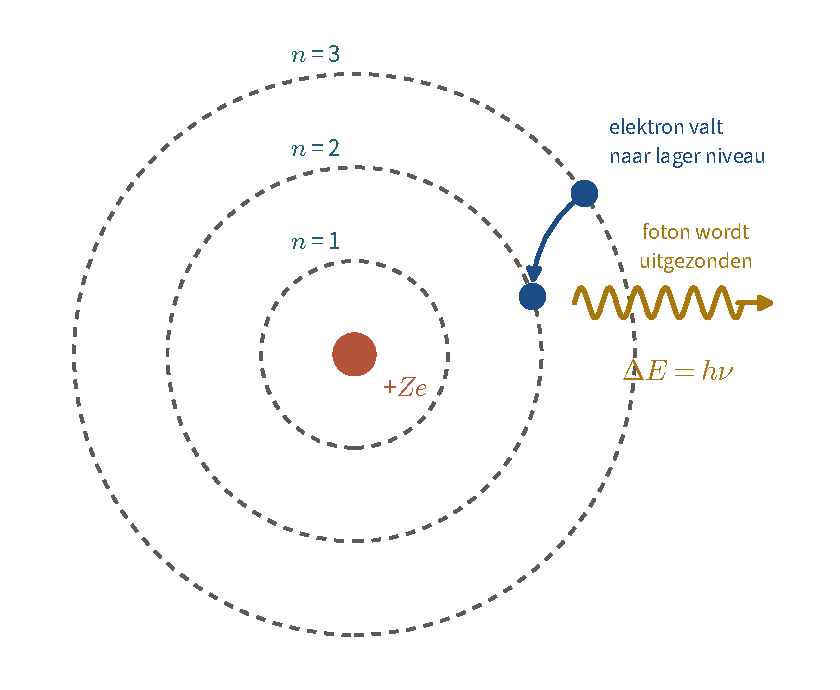
\includegraphics[width=0.5\linewidth]{Figuren/bohr}
    \caption{Schematische voorstelling van het model van Bohr: een elektron valt van baan $n=3$ naar $n=2$ en zendt een foton uit met $h\nu = \Delta E$.}
    \label{fig:bohr-model}
\end{figure}

\paragraph{De grenzen van het model.}
Toch bleek het model van Bohr ontoereikend, om drie fundamentele redenen:
\begin{enumerate}
\item Het werkt enkel voor systemen met precies één elektron (H, He$^+$, Li$^{2+}$). Voor elk atoom met meer elektronen geeft het verkeerde resultaten, omdat het de onderlinge afstoting van de elektronen niet beschrijft.
\item De kwantisatievoorwaarde~\eqref{eq:bohr-kwantisatie} wordt \emph{opgelegd} omdat ze het juiste antwoord geeft. Het model verklaart niet \emph{waarom} enkel die banen zijn toegelaten, en ook niet waarom een elektron op zo'n baan niet straalt.
\item Het beschrijft het elektron als een klassiek deeltje met een precieze plaats en snelheid op een baan. Dat beeld is onverenigbaar met het golfkarakter van materie (\S\ref{sec:materiegolf}).
\end{enumerate}
Een kleine aanpassing van de klassieke mechanica volstaat dus niet. Er was een nieuw kader nodig, waarin kwantisatie niet wordt opgelegd maar vanzelf uit de vergelijkingen volgt. Dat kader bouwen we in de volgende twee secties op.

\subsection{Atomaire spectra}
\label{sec:atomaire-spectra}

Valt een elektron terug naar een lager niveau, dan wordt het energieverschil uitgezonden als een foton met $h\nu = \Delta E$: een \emph{emissiespectrum}. Omgekeerd absorbeert een atoom enkel fotonen waarvan de energie precies overeenkomt met het verschil tussen twee niveaus: een \emph{absorptiespectrum}, met donkere lijnen bij dezelfde golflengten. Voor waterstof vat de formule van Rydberg, die we hierboven uit het model van Bohr afleidden, alle overgangen samen:
\begin{equation}
\boxed{
\frac{1}{\lambda} = R_H\left(\frac{1}{n_i^2}-\frac{1}{n_j^2}\right), \qquad n_j > n_i
}
\end{equation}
met $R_H = \SI{1.097e7}{\per\meter}$. Overgangen naar $n_i=1$ vormen de Lyman-reeks (UV), naar $n_i=2$ de Balmer-reeks (deels zichtbaar) en naar $n_i=3$ de Paschen-reeks (infrarood) (figuur~\ref{fig:waterstofspectrum}).

\begin{figure}[htb]
    \centering
    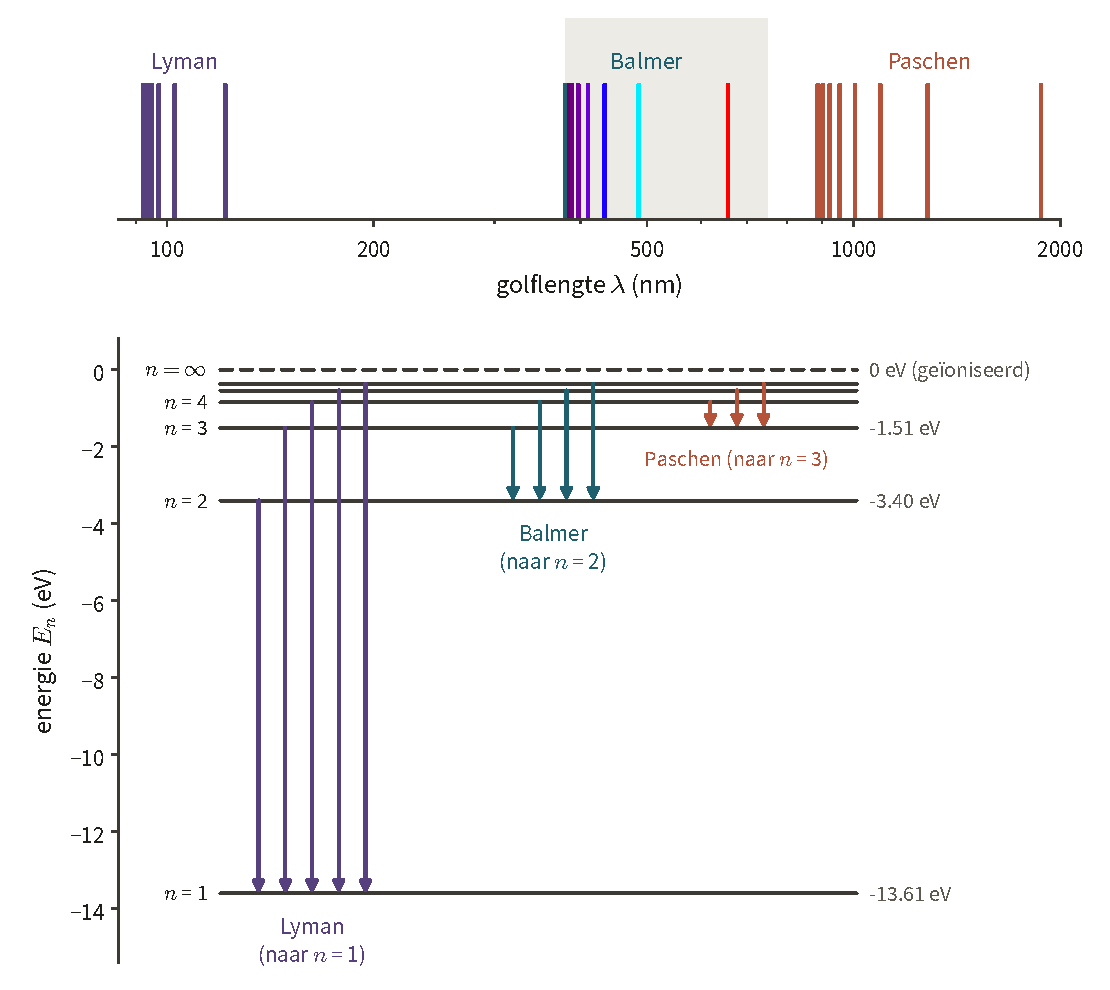
\includegraphics[width=0.62\linewidth]{Figuren/waterstof}
    \caption{Lijnenspectrum van waterstof (boven) en de overgangen tussen energieniveaus die het veroorzaken (onder): Lyman (naar $n=1$), Balmer (naar $n=2$) en Paschen (naar $n=3$).}
    \label{fig:waterstofspectrum}
\end{figure}

\begin{voorbeeld}{Twee lijnen van waterstof}
De overgang $n=2 \to n=1$ geeft $\Delta E = -3.40 - (-13.6) = \SI{10.2}{eV}$, dus
\[
\lambda = \frac{hc}{\Delta E} = \frac{(6.626\times 10^{-34})(2.998\times 10^{8})}{(10.2)(1.602\times 10^{-19})} = \SI{122}{\nano\meter},
\]
de eerste Lyman-lijn in het UV. De rode H$_\alpha$-lijn is de overgang $3 \to 2$:
\[
\frac{1}{\lambda} = (1.097\times10^{7})\left(\frac{1}{4}-\frac{1}{9}\right) = \SI{1.524e6}{\per\meter} \quad\Rightarrow\quad \lambda = \SI{656}{\nano\meter}.
\]
Sterrenkundigen herkennen waterstof in verre sterrenstelsels aan precies deze lijn.
\end{voorbeeld}

Elk element heeft andere energieniveaus en dus een eigen spectrum, een vingerafdruk. Dat zie je in het dagelijks leven: natriumdamp kleurt een vlam en de oude straatlampen geel (\SI{589}{\nano\metre}), neon gloeit rood-oranje, en vuurwerk krijgt zijn kleuren van strontium (rood), barium (groen) en koper (blauw). In het labo bepaalt men zo de samenstelling van een staal: in atoomemissie- en atoomabsorptiespectrometrie meet men de intensiteit van de lijnen van een element om zijn concentratie te bepalen, tot ver onder een milligram per liter.

\begin{casusuitgewerkt}{scherpe lijnen}
Een atoom of molecule kan enkel bepaalde energieën hebben. Het absorbeert dus enkel fotonen waarvan de energie precies overeenkomt met het verschil tussen twee toegelaten niveaus, $h\nu = \Delta E$. Daarom bestaat een spectrum uit scherpe lijnen.

Bij \SI{4.26}{\micro\metre} hoort
\[
\Delta E = \frac{hc}{\lambda} = \frac{(6.626\times10^{-34})(2.998\times10^{8})}{4.26\times10^{-6}} = \SI{4.66e-20}{\joule} = \SI{0.29}{\electronvolt} = \SI{28}{\kilo\joule\per\mole}.
\]
Dat is veel kleiner dan de elektronische overgangen van waterstof, die enkele elektronvolt bedragen (\SI{10.2}{\electronvolt} voor de eerste Lyman-lijn, \SI{1.9}{\electronvolt} voor H$_\alpha$). Bij de lijn van CO$_2$ verandert dus geen elektron van orbitaal. Er moeten nog andere, kleinere energietrappen bestaan: die van de molecule als geheel (\S\ref{sec:moleculaire-beweging}).

\emph{Volgende vraag.} Het model van Bohr legt de kwantisatie op zonder te verklaren waar ze vandaan komt. Waarom zijn de energieniveaus discreet?
\end{casusuitgewerkt}

\section{Materie als golf}
\label{sec:materiegolf}

Het antwoord op die vraag begint met een verrassende vaststelling: niet enkel licht, ook materie gedraagt zich als een golf.

\subsection{Golf of deeltje? Wat de experimenten toonden}

Rond 1920 lag er een verwarrende verzameling waarnemingen op tafel. Sommige experimenten toonden dat licht een golf is, andere dat het uit deeltjes bestaat. Kort daarna bleek hetzelfde te gelden voor elektronen (tabel~\ref{tab:dualiteit}).

\begin{table}[htb]
\centering
\caption{Waarnemingen die het duale karakter van licht en materie aantoonden.}
\label{tab:dualiteit}
\begin{tabular}{p{0.18\linewidth}p{0.36\linewidth}p{0.36\linewidth}}
\toprule
 & gedrag als golf & gedrag als deeltje \\
\midrule
licht & interferentie achter twee spleten (Young, 1801); buiging van röntgenstraling aan kristallen (Von Laue, Bragg, 1912) & foto-elektrisch effect (1905); botsing van röntgenfotonen met elektronen (Compton, 1923) \\
elektronen & buiging aan een nikkelkristal (Davisson en Germer, 1927) en aan dunne metaalfolie (Thomson, 1927) & sporen in een nevelkamer; afzonderlijke inslagen op een scherm \\
\bottomrule
\end{tabular}
\end{table}

\paragraph{Licht als golf.} Dat licht een golf is, leek sinds 1801 bewezen. Thomas Young liet licht door twee smalle spleten vallen en zag op een scherm een patroon van heldere en donkere banden. Waar de golven uit beide spleten in fase aankomen, versterken ze elkaar; waar een top een dal ontmoet, doven ze elkaar uit. Dat heet \emph{interferentie}, en enkel golven doen dat. Ook röntgenstraling buigt af aan de regelmatige rijen atomen in een kristal, wat de basis is van de röntgendiffractie waarmee men vandaag kristalstructuren bepaalt.

\paragraph{Licht als deeltje.} Het foto-elektrisch effect toonde dat licht zijn energie in pakketjes $h\nu$ afgeeft. In 1923 ging Arthur Compton een stap verder. Hij stuurde röntgenstraling op grafiet en zag dat de verstrooide straling een iets langere golflengte had, afhankelijk van de hoek. Dat kon hij enkel verklaren als een botsing tussen twee biljartballen: een foton botst op een elektron en geeft het een deel van zijn energie en zijn \emph{impuls} mee. Een foton heeft dus een impuls. Voor een deeltje zonder massa dat met de lichtsnelheid beweegt, is $E = pc$, en met $E = hc/\lambda$ volgt
\[
p = \frac{h}{\lambda}.
\]

\subsection{Het golfkarakter van materie}

\paragraph{De hypothese van De Broglie.}
In 1924, in zijn doctoraat, keerde Louis de Broglie die redenering om. Als licht, dat we als golf kenden, ook deeltjeseigenschappen heeft, dan heeft materie, die we als deeltjes kennen, misschien ook golfeigenschappen. Aan elk deeltje met impuls $p=mv$ kende hij dezelfde relatie toe als aan een foton:
\begin{equation}
\boxed{
\lambda=\frac{h}{p}=\frac{h}{mv}
}
\end{equation}
Dit betekent niet dat een elektron letterlijk als een klein, golvend draadje door de ruimte beweegt. Het betekent dat het gedrag van een deeltje beschreven wordt door een golf, en dat het onder geschikte omstandigheden interferentie en buiging vertoont. Voor macroscopische voorwerpen is de impuls zo groot dat de golflengte onmeetbaar klein is. Voor elektronen kan ze vergelijkbaar zijn met de afstand tussen atomen.

\begin{voorbeeld}{De De Broglie-golflengte van een elektron en een wandelende persoon}
Een elektron dat vanuit rust over een spanning $U$ wordt versneld, krijgt een kinetische energie $eU = \tfrac12 m_e v^2 = p^2/2m_e$. Zijn impuls is dus $p = \sqrt{2m_e eU}$, en zijn golflengte
\[
\lambda = \frac{h}{\sqrt{2m_e eU}} .
\]
Voor $U = \SI{150}{\volt}$:
\[
\lambda = \frac{6.626\times10^{-34}}{\sqrt{2(9.109\times10^{-31})(1.602\times10^{-19})(150)}} = \SI{1.00e-10}{\metre} = \SI{0.100}{\nano\metre},
\]
precies de afstand tussen atomen in een kristal. Zo'n elektronen buigen dus af aan een kristal, en de elektronenmicroscoop maakt hier gebruik van.

Een wandelaar ($m = \SI{75}{\kilo\gram}$, $v = \SI{1.5}{\metre\per\second}$) heeft $p = \SI{112.5}{\kilo\gram\metre\per\second}$ en
\[
\lambda = \frac{6.626\times10^{-34}}{112.5} = \SI{5.9e-36}{\metre},
\]
ontelbare grootteordes kleiner dan een atoomkern. Het golfkarakter van een mens is daarom volledig onwaarneembaar. De relatie van De Broglie geldt voor alle materie, maar ze wordt enkel merkbaar bij zeer lichte deeltjes.
\end{voorbeeld}

\paragraph{De bevestiging: elektronen buigen af.}
Drie jaar later werd de hypothese bevestigd, deels bij toeval. Clinton Davisson en Lester Germer schoten bij Bell Labs elektronen van \SI{54}{\electronvolt} loodrecht op een nikkelkristal en maten hoeveel elektronen onder elke hoek terugkaatsten (figuur~\ref{fig:davisson-germer}). Ze vonden een scherpe piek bij \SI{50}{\degree}, precies wat je verwacht voor een golf die buigt aan de rijen nikkelatomen. Een golf weerkaatst op die rijen, met onderlinge afstand $d = \SI{0.215}{\nano\metre}$, versterkt in de richting $\varphi$ waarvoor het wegverschil een hele golflengte is: $d\sin\varphi = \lambda$. Met de formule van De Broglie is
\[
\lambda = \frac{h}{\sqrt{2m_e eU}} = \SI{0.167}{\nano\metre}
\quad\Longrightarrow\quad
\sin\varphi = \frac{0.167}{0.215} = 0.776, \quad \varphi = \SI{51}{\degree}.
\]
Vrijwel tegelijk stuurde George Thomson elektronen door een dunne goudfolie en zag hij ringen zoals bij röntgenstraling. Sindsdien is interferentie aangetoond met neutronen, heliumatomen en zelfs met voetbalvormige C$_{60}$-moleculen van 60 koolstofatomen.

\begin{figure}[htb]
    \centering
    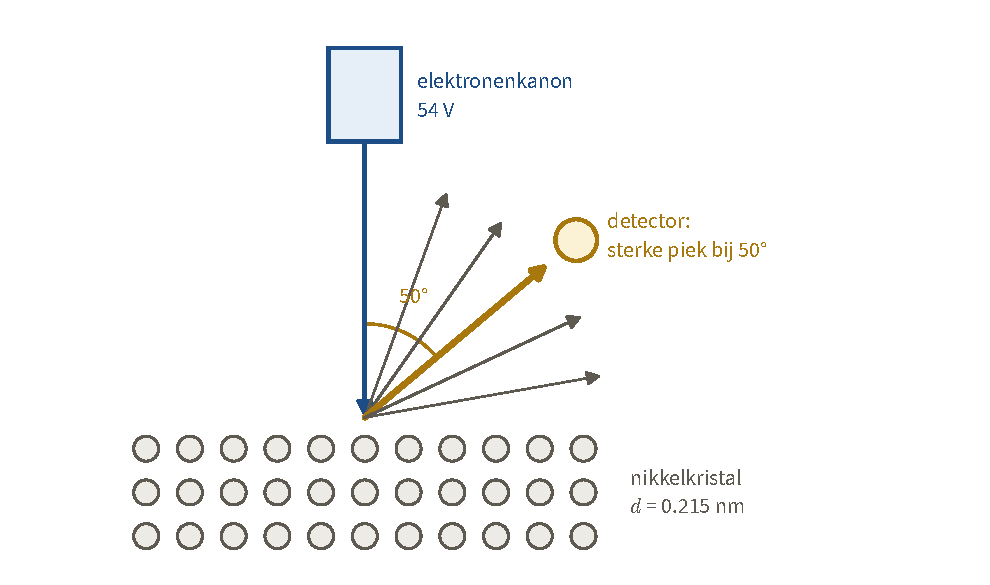
\includegraphics[width=0.62\linewidth]{Figuren/davisson_germer}
    \caption{Het experiment van Davisson en Germer (1927). Elektronen van \SI{54}{\electronvolt} worden door een nikkelkristal sterk teruggekaatst onder een hoek van \SI{50}{\degree}: ze buigen af als golven met de golflengte van De Broglie.}
    \label{fig:davisson-germer}
\end{figure}

\subsection{De dubbelspleetproef}
\label{sec:dubbelspleet}

De meest overtuigende proef is de dubbelspleetproef van Young, maar dan met elektronen. Stuur je een elektronenbundel door twee fijne spleten, dan ontstaat op een scherm een interferentiepatroon van heldere en donkere banden, zoals bij licht. Dat patroon is enkel te verklaren als elk elektron zich als een golf door \emph{beide} spleten tegelijk beweegt: de twee deelgolven versterken of doven elkaar op het scherm.

Het wordt nog vreemder wanneer de bron zo zwak is dat er telkens maar één elektron onderweg is. Dan verschijnt op het scherm telkens één scherp punt: het elektron wordt als deeltje gedetecteerd, op één plaats. Waar het volgende elektron aankomt, is niet te voorspellen. Pas na duizenden elektronen ontstaat het patroon van banden (figuur~\ref{fig:dubbelespleet}). Elk afzonderlijk elektron gedraagt zich dus bij de detectie als een deeltje, maar de verdeling van vele inslagen is die van een golf. Probeer je te meten door welke spleet een elektron gaat, dan verdwijnt het patroon. Licht en materie zijn dus geen golf óf deeltje; ze vertonen beide aspecten, afhankelijk van wat je meet.

\begin{figure}[htb]
    \centering
    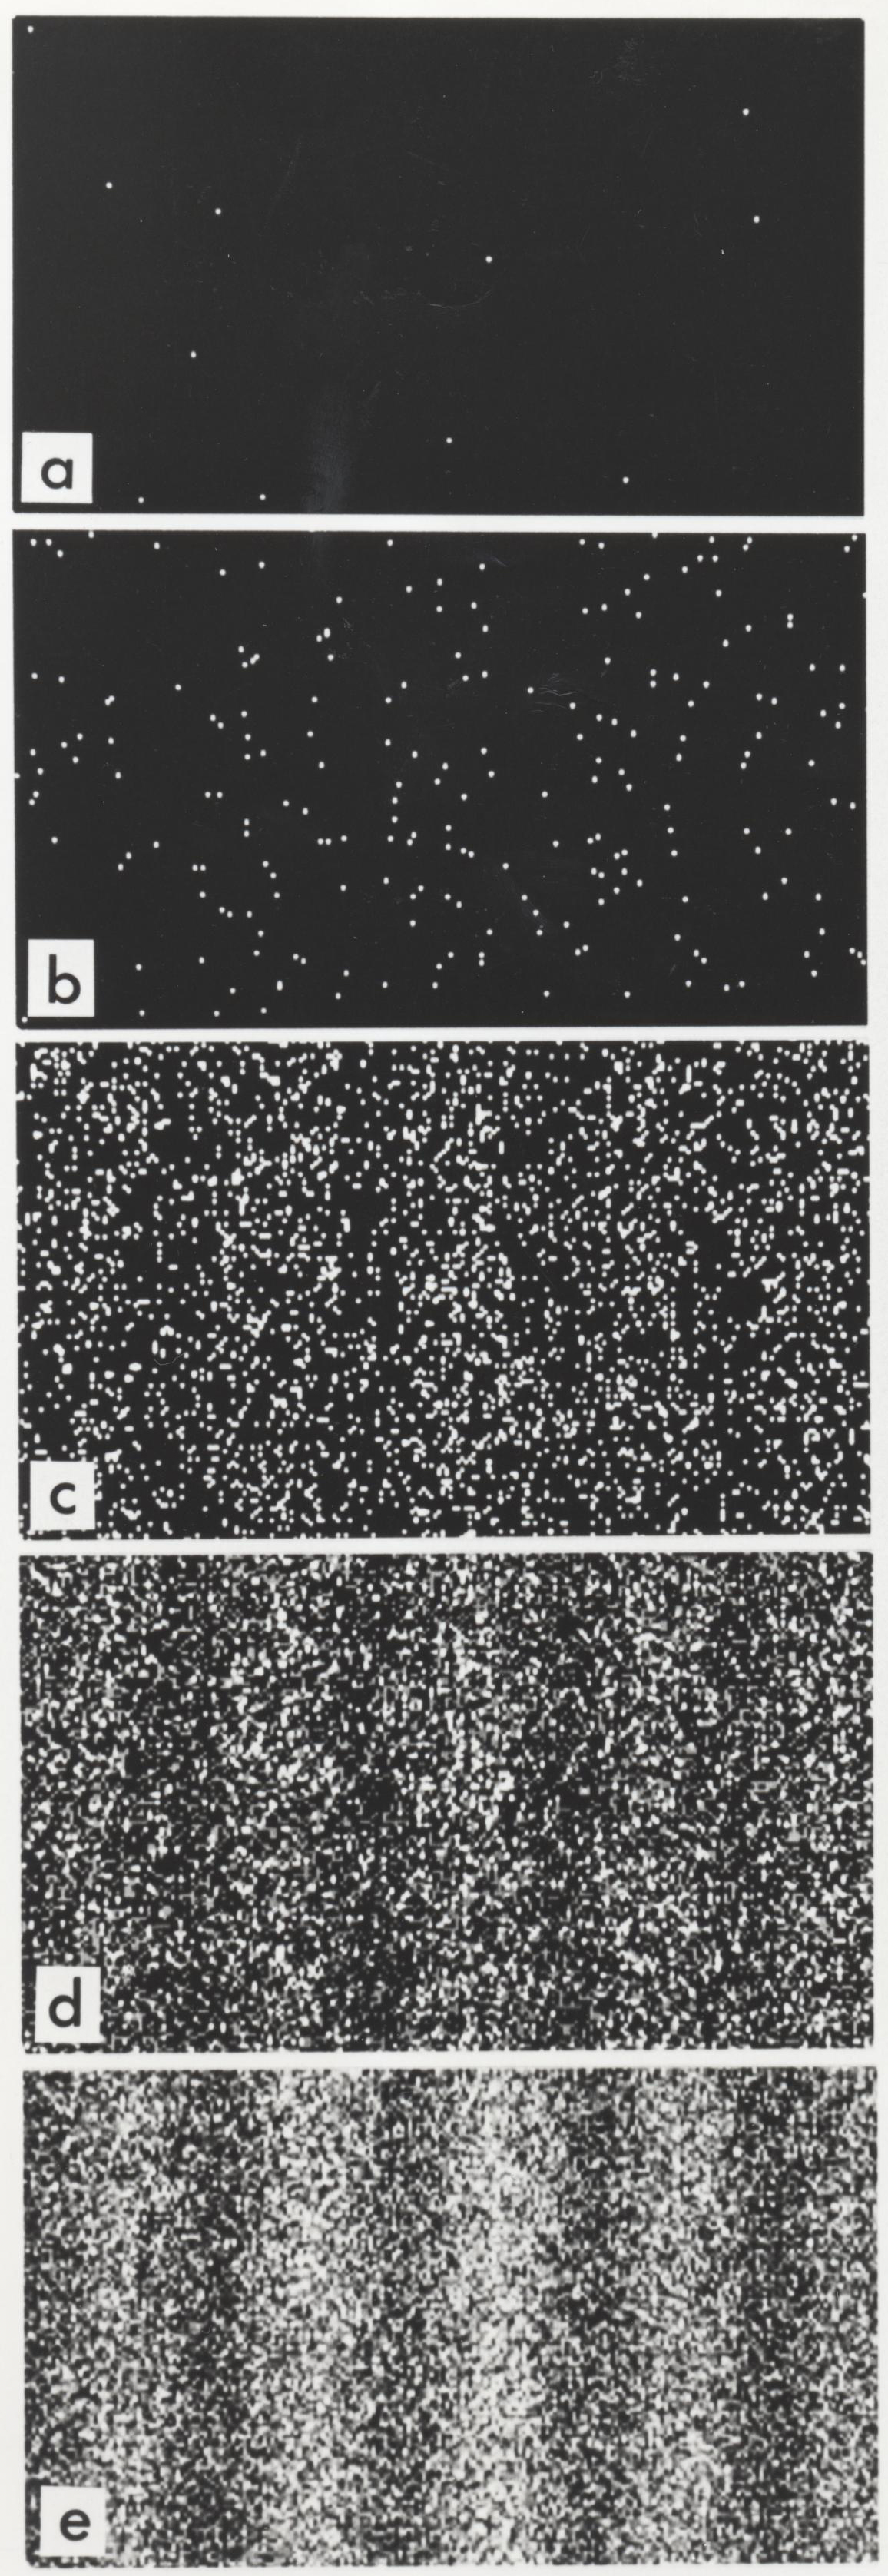
\includegraphics[width=0.3\linewidth]{Afbeeldingen/Double-slit_experiment_results_Tonomura_2.jpg}
    \caption{Dubbelspleetexperiment met afzonderlijke elektronen: na 11 (a), 200 (b), 6000 (c), 40\,000 (d) en 140\,000 (e) elektronen.}
    \label{fig:dubbelespleet}
\end{figure}

\begin{toepassing}{Een Brussels weetje: de Solvayconferentie van 1927}
Ernest Solvay, rijk geworden met zijn sodaproces (\ce{Na2CO3}, nog steeds de basis van de glasindustrie), financierde vanaf 1911 de Solvayconferenties voor natuurkunde in Brussel. De vijfde, in oktober 1927, ging over ``elektronen en fotonen''. Op de groepsfoto staan onder meer Einstein, Bohr, Planck, Marie Curie, Schr\"odinger, Heisenberg, De Broglie, Dirac en Pauli: 17 van de 29 deelnemers hadden of kregen een Nobelprijs. Er werd hevig gediscussieerd over de betekenis van de golffunctie, het onderwerp van de volgende sectie. Einsteins ``God dobbelt niet'' en Bohrs antwoord ``Einstein, vertel God niet wat Hij moet doen'' stammen uit die discussies.
\end{toepassing}

\section{De golffunctie en de Schr\"odingervergelijking}

\subsection{De golffunctie en haar betekenis}
\label{sec:golffunctie}

\paragraph{Wat beschrijft een golf?}
Elke golf wordt beschreven door een functie die op elke plaats en elk tijdstip de \emph{amplitude} geeft: de uitwijking van een gitaarsnaar $y(x,t)$, de luchtdruk bij geluid, of bij licht de elektrische veldsterkte. Die amplitude kan positief of negatief zijn: een snaar wijkt naar boven of naar onder uit. Wat je waarneemt, is echter niet de amplitude zelf, maar de \emph{intensiteit}, de energie die per seconde aankomt. Die is evenredig met het \emph{kwadraat} van de amplitude. Een lichtmeter of je oog meet dus amplitude in het kwadraat.

Denk nu aan fotonen. Laat je heel zwak licht op een fotoplaat vallen, dan komen de fotonen één voor één aan, elk op één punt. Waar de amplitude groot is, komen er veel aan; waar ze nul is, geen. Het kwadraat van de amplitude zegt dus \emph{hoe waarschijnlijk} het is dat een foton op een bepaalde plaats aankomt.

\paragraph{De golffunctie van een elektron.}
In de kwantummechanica wordt de toestand van een elektron, of van elk ander deeltje, beschreven door een \emph{golffunctie} $\psi(\vec r, t)$: de amplitude van de materiegolf op elke plaats $\vec r$ en elk tijdstip $t$. De golffunctie bevat alle informatie die over het deeltje te kennen is. Ze is zelf geen meetbare grootheid; je kunt nergens ``$\psi$ aflezen''. Ze kan positief of negatief zijn, en in het algemeen is ze zelfs een \emph{complex} getal.

Waarom complex? Een golf heeft op elke plaats twee kenmerken: hoe groot de uitwijking is (de amplitude) en waar in de trilling ze zit (de \emph{fase}: op een top, in een dal, of ertussen). Een complex getal $\psi = |\psi|\,e^{i\phi}$ draagt die twee in één getal. Voor een elektron dat met welbepaalde impuls $p = \hbar k$ in de $x$-richting beweegt, is de golffunctie $\psi = A\,e^{i(kx-\omega t)}$. Het reële en het imaginaire deel zijn dan een cosinus- en een sinusgolf die een kwart golflengte verschoven zijn (figuur~\ref{fig:golffunctie}a).

\paragraph{De betekenis van $\psi^*\psi$.}
Max Born gaf in 1926 de interpretatie, naar analogie met de fotonen: het kwadraat van de amplitude is een kans. Omdat $\psi$ complex kan zijn, neem je niet gewoon $\psi^2$, maar het product van $\psi$ met zijn \emph{complex toegevoegde} $\psi^*$. Schrijf je $\psi = a + ib$, dan is $\psi^* = a - ib$ en
\[
\psi^*\psi = (a-ib)(a+ib) = a^2 + b^2 = |\psi|^2 .
\]
Dat is altijd een reëel, positief getal, zoals een kans moet zijn. Het wordt de \emph{waarschijnlijkheidsdichtheid} genoemd: de kans per volume-eenheid om het deeltje op die plaats aan te treffen (eenheid \si{\per\metre\cubed}). De kans om het deeltje op tijdstip $t$ in een klein volume $\dd V$ rond $\vec r$ te vinden, is
\begin{equation}
\boxed{
\dd P = \psi^*(\vec{r},t)\,\psi(\vec{r},t)\,\dd V = |\psi(\vec{r},t)|^2\,\dd V .
}
\end{equation}
De kans om het in een groter gebied $\Omega$ te vinden, is de integraal over dat gebied, het oppervlak onder de kromme in figuur~\ref{fig:golffunctie}b:
\[
P_\Omega = \int_\Omega |\psi|^2\,\dd V .
\]
Omdat het deeltje zich ergens moet bevinden, is de totale kans gelijk aan één:
\begin{equation}
\int_{\text{volledige ruimte}} |\psi|^2\,\dd V = 1 .
\label{eq:normering}
\end{equation}
Een golffunctie die hieraan voldoet, heet \emph{genormeerd}.

\begin{figure}[htb]
    \centering
    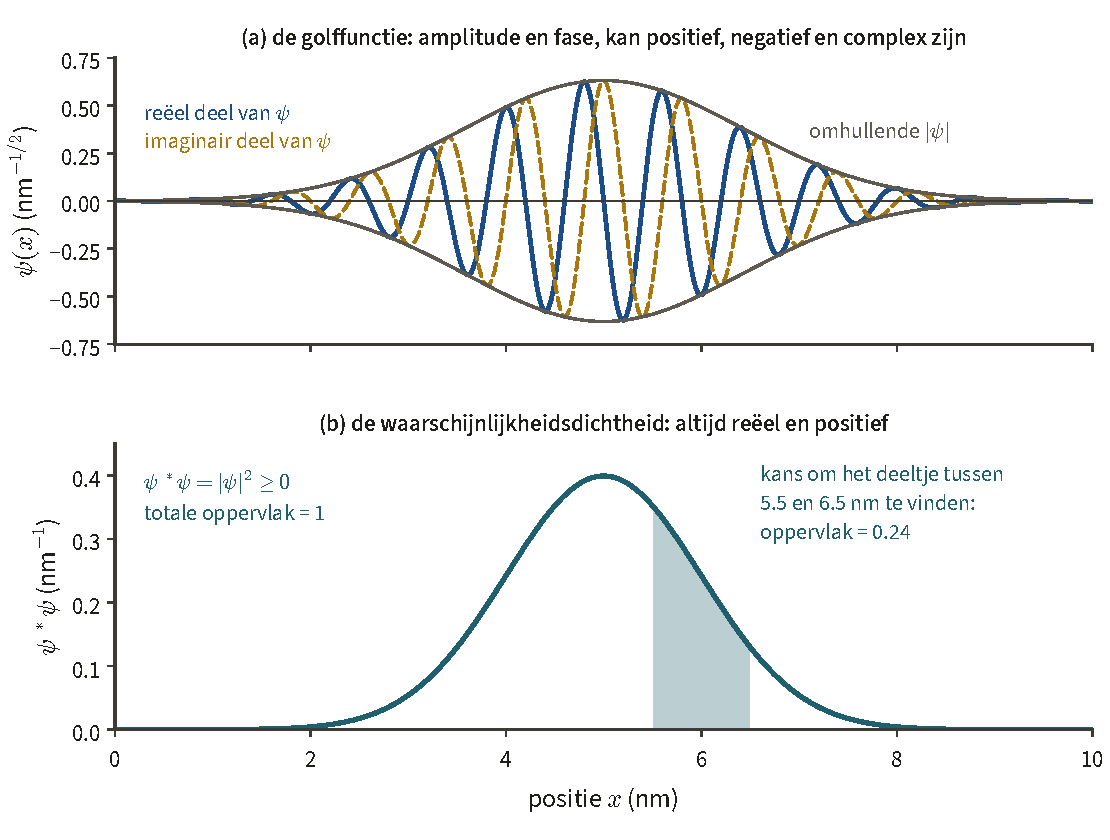
\includegraphics[width=0.8\linewidth]{Figuren/golffunctie_betekenis}
    \caption{(a) De golffunctie van een elektron dat in een beperkt gebied naar rechts beweegt. Het reële en het imaginaire deel trillen een kwart golflengte verschoven; de omhullende $|\psi|$ geeft de grootte. (b) De waarschijnlijkheidsdichtheid $\psi^*\psi$. De fase valt weg, en wat overblijft is altijd positief. Het gearceerde oppervlak is de kans om het elektron tussen \SI{5.5}{} en \SI{6.5}{\nano\metre} aan te treffen.}
    \label{fig:golffunctie}
\end{figure}

Voor de golf $\psi = A\,e^{i(kx-\omega t)}$ van een elektron met welbepaalde impuls is $\psi^*\psi = A\,e^{-i(kx-\omega t)}\,A\,e^{i(kx-\omega t)} = A^2$: overal even groot. Een elektron waarvan de impuls exact gekend is, kan overal zijn. Wil je het lokaliseren, zoals in figuur~\ref{fig:golffunctie}, dan moet je golven met verschillende impulsen combineren. Plaats en impuls zijn dus nooit tegelijk exact bepaald; dat is de \emph{onzekerheidsrelatie} van Heisenberg.

\paragraph{Waarom de fase er toch toe doet.}
In $\psi^*\psi$ valt de fase weg. Toch is ze belangrijk zodra twee golven samenkomen. In de dubbelspleetproef is de golffunctie op het scherm de som $\psi = \psi_1 + \psi_2$ van de golven uit elke spleet, en de kans is $|\psi_1 + \psi_2|^2$, niet $|\psi_1|^2 + |\psi_2|^2$. Waar beide in fase aankomen, versterken ze elkaar; waar ze tegengesteld zijn, wordt de kans nul. Dat is de oorsprong van de donkere banden. Hetzelfde mechanisme vormt verderop de chemische binding: twee atoomorbitalen die in fase overlappen, vergroten de kans om het elektron tussen de kernen te vinden (\S\ref{sec:molecuulorbitalen}).

De kwantummechanica voorspelt dus niet waar één elektron zal worden aangetroffen, wel hoe vaak elke plaats voorkomt als je de meting vele keren herhaalt. Dat is precies wat de dubbelspleetproef toont: elke inslag is willekeurig, maar de verdeling volgt $|\psi|^2$. Het is ook de eerste keer in deze cursus dat waarschijnlijkheid een fundamentele rol speelt, in plaats van onze onwetendheid te weerspiegelen. In hoofdstuk~\ref{ch:spontaniteit} ligt diezelfde idee, een groot aantal mogelijke toestanden met elk een waarschijnlijkheid, aan de basis van de entropie.

\subsection{De Schr\"odingervergelijking}

\paragraph{Waar komt de vergelijking vandaan?}
De golffunctie zegt wat we kunnen weten, maar welke golffuncties zijn mogelijk voor een elektron in een atoom of een molecule? Erwin Schr\"odinger stelde daarvoor in 1926 een vergelijking op. Ze kan niet worden afgeleid uit de klassieke fysica, maar je kunt wel zien waarom ze deze vorm heeft.

Neem een vrij deeltje met impuls $p$. Volgens De Broglie hoort daar een golf bij met golflengte $\lambda = h/p$, bijvoorbeeld $\psi = A\sin(kx)$ met golfgetal $k = 2\pi/\lambda = p/\hbar$. Leid je die golf twee keer af, dan krijg je
\[
\frac{\dd^2\psi}{\dd x^2} = -k^2\psi = -\frac{p^2}{\hbar^2}\,\psi .
\]
Vermenigvuldig met $-\hbar^2/2m$ en gebruik dat de kinetische energie $p^2/2m$ is:
\[
-\frac{\hbar^2}{2m}\frac{\dd^2\psi}{\dd x^2} = \frac{p^2}{2m}\,\psi = E_\mathrm{kin}\,\psi .
\]
Is er ook een potentiële energie $V$, dan is $E_\mathrm{kin} = E - V$, met $E$ de totale energie. Schr\"odinger postuleerde dat deze relatie ook geldt wanneer $V$ van plaats tot plaats verandert. Zo krijg je, voor één deeltje in één dimensie en een toestand met welbepaalde energie, de \emph{tijdsonafhankelijke Schr\"odingervergelijking}:
\begin{equation}
\boxed{
-\frac{\hbar^2}{2m}\frac{\partial^2\psi}{\partial x^2} + V(x)\psi = E\psi,
}
\label{eq:Schrodinger}
\end{equation}
met $\hbar=h/2\pi$, $m$ de massa van het deeltje, $V(x)$ de potentiële energie en $E$ de totale energie.

\paragraph{Wat de vergelijking zegt.}
De eerste term is de kinetische energie, en die hangt af van de \emph{kromming} van $\psi$. Waar $E - V$ groot is, beweegt het deeltje snel: de golf is daar sterk gekromd, met een korte golflengte. Waar $E - V$ klein is, is de golf vlakker. En waar $V > E$, een gebied dat klassiek verboden is, kromt de golf de andere kant op: ze trilt niet meer, maar sterft exponentieel uit. Het deeltje dringt dus een klein stukje door in een gebied waar het klassiek niet mag komen. Is zo'n gebied dun genoeg, dan kan het er zelfs doorheen: het \emph{tunneleffect}, waarop de rastertunnelmicroscoop en het geheugen in een usb-stick berusten.

De Schr\"odingervergelijking speelt dezelfde rol als de wetten van Newton in de klassieke mechanica. Ze levert echter geen baan of exacte positie, maar de golffuncties die voor het systeem mogelijk zijn, en de bijbehorende energieën.

\paragraph{Welke oplossingen zijn toegelaten?}
Niet elke wiskundige oplossing van~\eqref{eq:Schrodinger} beschrijft een fysische toestand. Een aanvaardbare golffunctie moet aan drie voorwaarden voldoen:
\begin{itemize}
\item \textbf{Eindig}: $\psi$ mag nergens oneindig worden, want dan zou $|\psi|^2$ een oneindige kans per volume geven op die plaats, wat fysisch onmogelijk is.
\item \textbf{Continu}: $\psi$ mag geen sprongen maken, en bij een eindige potentiaal ook haar eerste afgeleide niet. De vergelijking bevat een tweede afgeleide, en die bestaat enkel als $\psi$ vloeiend verloopt.
\item \textbf{Normeerbaar}: de totale kans~\eqref{eq:normering} moet gelijk aan één kunnen worden gemaakt. Voor een gebonden deeltje moet $\psi$ daarom naar nul gaan op grote afstand.
\end{itemize}
Juist deze voorwaarden laten voor een opgesloten deeltje slechts bepaalde golffuncties toe, en dus slechts bepaalde energieën. De kwantisatie is geen extra postulaat meer zoals bij Bohr; ze volgt uit de vergelijking zelf. Dat maken we in de volgende paragraaf concreet.

Voor een elektron in een atoom is $V$ de Coulombaantrekking door de kern. De oplossingen zijn de atoomorbitalen en hun energieniveaus (\S\ref{sec:waterstofatoom}). Verderop passen we dezelfde vergelijking toe op heel andere potentialen: een molecule die vrij beweegt in een vat, die roteert of die trilt (\S\ref{sec:moleculaire-beweging}). Telkens volgen er vanzelf discrete energieniveaus en nieuwe kwantumgetallen uit.

Ook de stabiliteit van het atoom volgt nu. Een toestand met welbepaalde energie heeft een kansverdeling $|\psi|^2$ die niet verandert in de tijd: er beweegt geen lading heen en weer, en er wordt dus niets uitgestraald. De laagste toegelaten oplossing is de grondtoestand. Een toestand waarin het elektron in de kern stort, is geen aanvaardbare oplossing: hij zou een oneindig sterk gekromde golffunctie vereisen, met een oneindige kinetische energie.

\subsection{Discrete energieniveaus}
\label{sec:discrete-energieniveaus}

Een gitaarsnaar die aan beide uiteinden vastzit, kan enkel trillen in patronen met een geheel aantal halve golflengten, net zoals het stralingsveld in de holte van figuur~\ref{fig:trillingsmodi}. Voor een materiegolf die opgesloten zit, geldt hetzelfde. Dat maken we concreet met het eenvoudigste voorbeeld: een deeltje met massa $m$ dat vrij beweegt in een ééndimensionale \emph{doos} met lengte $L$, en de wanden niet kan verlaten ($V=0$ binnen, $V=\infty$ buiten).

\emph{Stap 1: de vergelijking.} Binnen de doos is $V=0$ en wordt~\eqref{eq:Schrodinger}
\[
-\frac{\hbar^2}{2m}\frac{\dd^2\psi}{\dd x^2} = E\psi
\qquad\text{of}\qquad
\frac{\dd^2\psi}{\dd x^2} = -k^2\psi, \quad k=\frac{\sqrt{2mE}}{\hbar}.
\]
Welke functie geeft na twee keer afleiden zichzelf terug, met een minteken? Een sinus en een cosinus. De algemene oplossing is dus $\psi(x)=A\sin(kx)+B\cos(kx)$.

\emph{Stap 2: de randvoorwaarden.} Buiten de doos is $\psi = 0$, want het deeltje kan er niet zijn. Omdat $\psi$ continu moet zijn, moet ze ook aan de wanden nul zijn: $\psi(0)=0$ en $\psi(L)=0$. De eerste voorwaarde geeft $B=0$, want $\cos 0 = 1$. De tweede geeft $A\sin(kL)=0$. Met $A=0$ zou er geen deeltje zijn, dus moet $\sin(kL)=0$:
\[
kL = n\pi, \qquad n=1,2,3,\ldots
\]
Er passen dus een geheel aantal halve golflengten in de doos, $L = n\lambda/2$, net als bij de snaar.

\emph{Stap 3: de energie.} Met $k = n\pi/L$ in $E=\hbar^2k^2/(2m)$ volgt
\begin{equation}
\boxed{
E_n = \frac{n^2h^2}{8mL^2}, \qquad n=1,2,3,\ldots
}
\label{eq:deeltje-in-doos}
\end{equation}

\emph{Stap 4: de normering.} De constante $A$ volgt uit~\eqref{eq:normering}: $\int_0^L A^2\sin^2(n\pi x/L)\,\dd x = A^2 L/2 = 1$, dus $A = \sqrt{2/L}$ en
\[
\psi_n(x) = \sqrt{\frac{2}{L}}\,\sin\frac{n\pi x}{L}.
\]

De kwantisatie volgt hier uitsluitend uit de randvoorwaarden; er is geen extra postulaat nodig zoals bij Bohr. Figuur~\ref{fig:deeltje-doos} toont de eerste vier oplossingen. Drie eigenschappen komen in elk kwantumsysteem terug:
\begin{itemize}
\item De laagste energie is \emph{niet nul}: $E_1 = h^2/(8mL^2)$. Een opgesloten deeltje kan nooit volledig stilliggen. Deze \emph{nulpuntsenergie} vinden we terug bij de trillende molecule (\S\ref{sec:vibratie}).
\item Hogere toestanden hebben meer \emph{knopen}, punten waar $\psi = 0$: toestand $n$ heeft er $n-1$. Meer knopen betekent een sterker gekromde golf, dus een hogere kinetische energie.
\item De niveaus liggen verder uit elkaar naarmate de doos kleiner of het deeltje lichter is ($E_n \propto 1/mL^2$). Daarom is kwantisatie belangrijk voor elektronen in atomen en verwaarloosbaar voor een knikker in een doos.
\end{itemize}

\begin{figure}[htb]
    \centering
    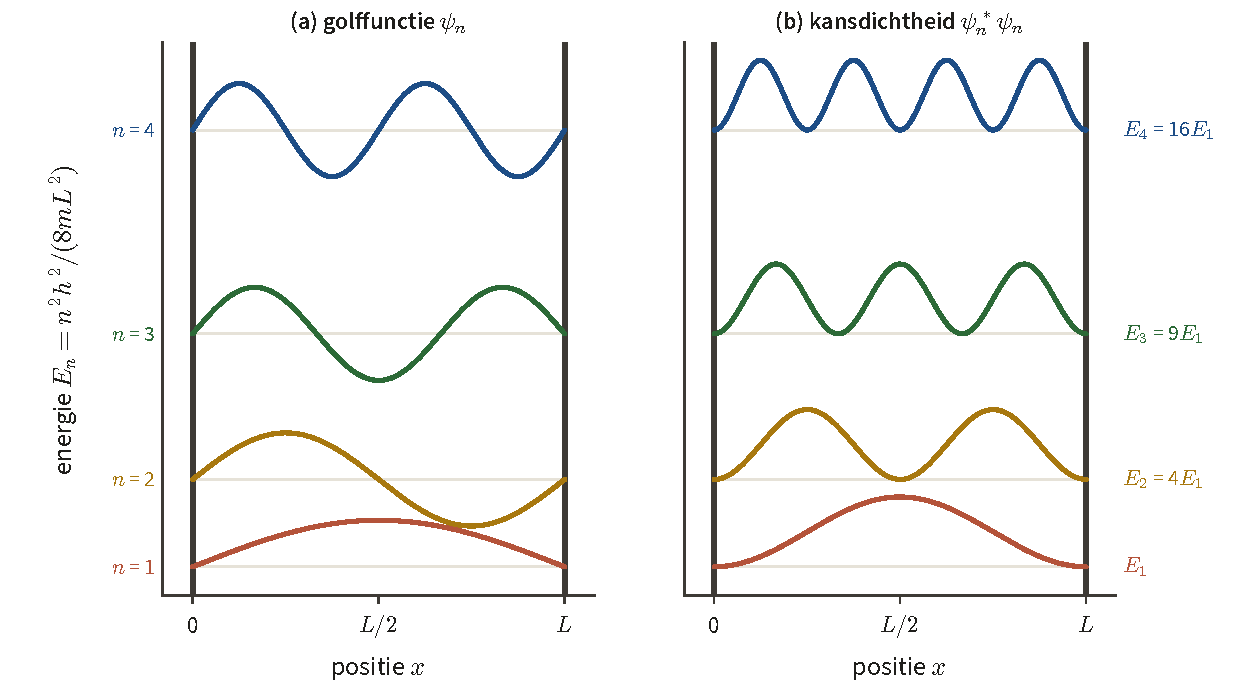
\includegraphics[width=0.85\linewidth]{Figuren/deeltje_doos}
    \caption{Deeltje in een doos. (a) De golffuncties van de eerste vier toestanden, elk getekend op de hoogte van zijn energie $E_n = n^2E_1$. (b) De waarschijnlijkheidsdichtheden $\psi_n^*\psi_n$. In toestand $n=2$ is de kans om het deeltje in het midden te vinden nul.}
    \label{fig:deeltje-doos}
\end{figure}

\begin{voorbeeld}{Waar zit het deeltje, en hoe groot zijn de energiesprongen?}
\emph{Kans in het middelste derde.} In de grondtoestand is de kans om het deeltje tussen $L/3$ en $2L/3$ te vinden
\[
P = \int_{L/3}^{2L/3}\frac{2}{L}\sin^2\frac{\pi x}{L}\,\dd x = \frac13 + \frac{\sqrt3}{2\pi} = 0.61 .
\]
Een klassiek deeltje dat heen en weer botst, zou even vaak op elke plaats zijn, met een kans van $1/3$. Het kwantumdeeltje in de grondtoestand zit liever in het midden. In toestand $n=2$ is de kans in het exacte midden nul, hoewel het deeltje links en rechts ervan wel kan zijn.

\emph{Een elektron in een doos van \SI{1}{\nano\metre}.} Dat is ongeveer de lengte van een molecule met een rij geconjugeerde dubbele bindingen. Dan is
\[
E_1 = \frac{(6.626\times10^{-34})^2}{8(9.109\times10^{-31})(1.0\times10^{-9})^2} = \SI{6.0e-20}{\joule} = \SI{0.38}{\electronvolt},
\]
en de sprong van $n=1$ naar $n=2$ is $3E_1 = \SI{1.1}{\electronvolt}$, een foton van \SI{1.1}{\micro\metre}. Hoe kleiner de doos, hoe groter de sprong en hoe blauwer het licht. Dat is het principe van \emph{quantum dots}: halfgeleiderkristalletjes van enkele nanometer waarvan de kleur enkel door hun grootte wordt bepaald, gebruikt in de beeldschermen van QLED-televisies.
\end{voorbeeld}

We gebruiken dit resultaat verderop voor de translatie van een molecule in een vat (\S\ref{sec:translatie}).

\subsection{Het waterstofatoom: energieniveaus en orbitalen}
\label{sec:waterstofatoom}

\paragraph{Energieniveaus.}
Voor het waterstofatoom is $V(r)= -e^2/(4\pi\varepsilon_0 r)$, de Coulombaantrekking tussen kern en elektron, nu in drie dimensies. De Schr\"odingervergelijking kan voor deze potentiaal exact worden opgelost. De wiskunde laten we achterwege, maar het resultaat is opvallend: de energieniveaus hangen enkel af van een geheel getal $n$, het hoofdkwantumgetal,
\begin{equation}
E_n = -\frac{\SI{13.6}{eV}}{n^2}, \qquad n = 1,2,3,\ldots
\end{equation}
Het minteken betekent dat het elektron gebonden is. De grondtoestand heeft $E_1 = \SI{-13.6}{eV}$, dan volgen $E_2 = \SI{-3.40}{eV}$ en $E_3 = \SI{-1.51}{eV}$; voor grote $n$ nadert de energie nul. Dat zijn precies de niveaus van Bohr~\eqref{eq:bohr-energie}, maar nu volgt de kwantisatie uit de voorwaarden op de golffunctie, zoals bij het deeltje in een doos. Het model van Bohr was dus een gelukkige gok. De Schr\"odingervergelijking verklaart daarnaast ook atomen met meer elektronen en moleculen, waar Bohr faalde.

\paragraph{Van golffunctie naar orbitaal.}
De oplossingen van de Schr\"odingervergelijking voor een elektron in een atoom heten \emph{atoomorbitalen}. Een orbitaal is dus een toegelaten golffunctie, geen baan. Het elektron draait niet zoals bij Bohr op een cirkel rond de kern; het orbitaal geeft via $|\psi|^2$ aan waar de kans groot of klein is om het elektron aan te treffen. Teken je die kans in drie dimensies, dan krijg je een \emph{elektronenwolk}. Die wolk is geen materiële wolk waarin de lading letterlijk uitgesmeerd is: bij elke meting vind je het elektron op één plaats, maar over vele metingen vormen de plaatsen deze wolk.

Het eenvoudigste orbitaal is de grondtoestand van waterstof, het \emph{1s-orbitaal}:
\[
\psi_{1s}(r) = \frac{1}{\sqrt{\pi a_0^3}}\,e^{-r/a_0},
\]
met $a_0 = \SI{52.9}{\pico\metre}$, opnieuw de straal van Bohr. Het hangt enkel af van de afstand $r$ tot de kern, niet van de richting: het orbitaal is bolvormig. De kans per volume $|\psi_{1s}|^2$ is het grootst in de kern zelf en daalt exponentieel naar buiten (figuur~\ref{fig:radiale-1s}). Betekent dit dat het elektron het vaakst in de kern zit? Nee. Op afstand $r$ ligt een bolschil met dikte $\dd r$ en volume $4\pi r^2\,\dd r$. Hoe verder van de kern, hoe groter die schil. De kans om het elektron op een afstand tussen $r$ en $r+\dd r$ te vinden, is daarom
\[
P(r)\,\dd r = 4\pi r^2\,|\psi_{1s}|^2\,\dd r = \frac{4r^2}{a_0^3}\,e^{-2r/a_0}\,\dd r .
\]
Dicht bij de kern is de schil zeer klein, ver weg is $|\psi|^2$ zeer klein; ertussen ligt een maximum. Stel je de afgeleide van $r^2e^{-2r/a_0}$ gelijk aan nul, dan vind je $2r - 2r^2/a_0 = 0$, dus $r = a_0$. De meest waarschijnlijke afstand tussen het elektron en de kern is exact de straal van Bohr. Het oude model had dus een kern van waarheid: de baan van Bohr is de plaats waar de elektronenwolk het dichtst is.

\begin{figure}[htb]
    \centering
    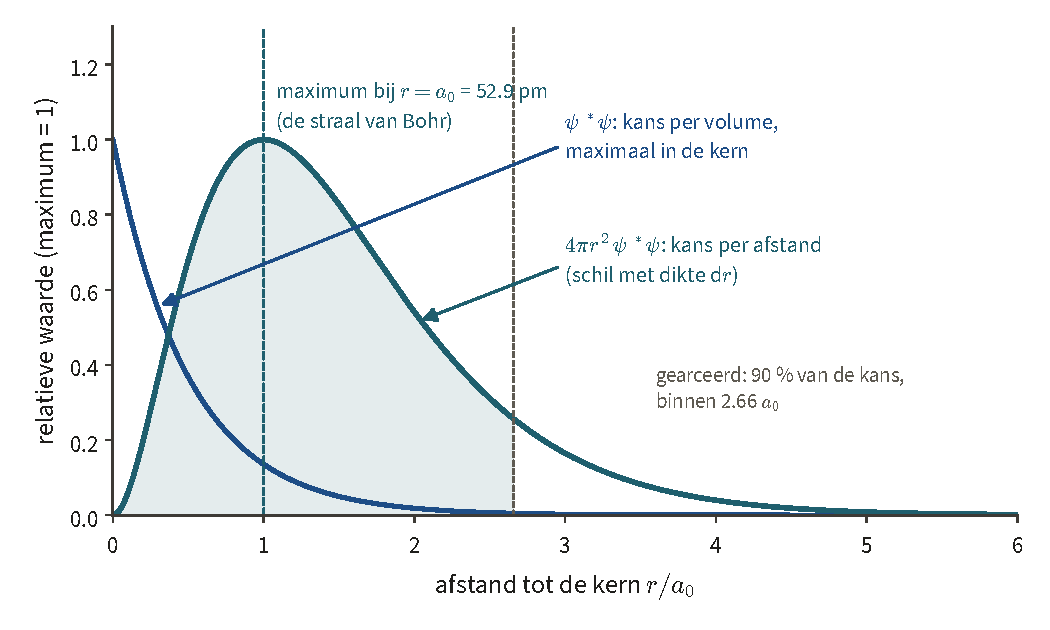
\includegraphics[width=0.7\linewidth]{Figuren/radiale_1s}
    \caption{Het 1s-orbitaal van waterstof. De kans per volume $\psi^*\psi$ is maximaal in de kern, maar de kans per afstand $4\pi r^2\psi^*\psi$ is maximaal bij $r = a_0$, de straal van Bohr. Binnen $2.66\,a_0$ ligt \SI{90}{\percent} van de kans.}
    \label{fig:radiale-1s}
\end{figure}

Een wolk heeft geen scherpe rand. Om toch een vorm te tekenen, kiest men het oppervlak dat bijvoorbeeld \SI{90}{\percent} van de kans omsluit; voor het 1s-orbitaal is dat een bol met straal $2.66\,a_0 = \SI{141}{\pico\metre}$. Voor hogere energieniveaus heeft de Schr\"odingervergelijking ook oplossingen die van de richting afhangen. Zo ontstaan de halter-vormige $p$-orbitalen en de klavervormige $d$-orbitalen (figuur~\ref{fig:orbitalen}). Welke orbitalen bij elk niveau horen, wordt bepaald door drie kwantumgetallen, het onderwerp van de volgende sectie.

\begin{figure}[htb]
    \centering
    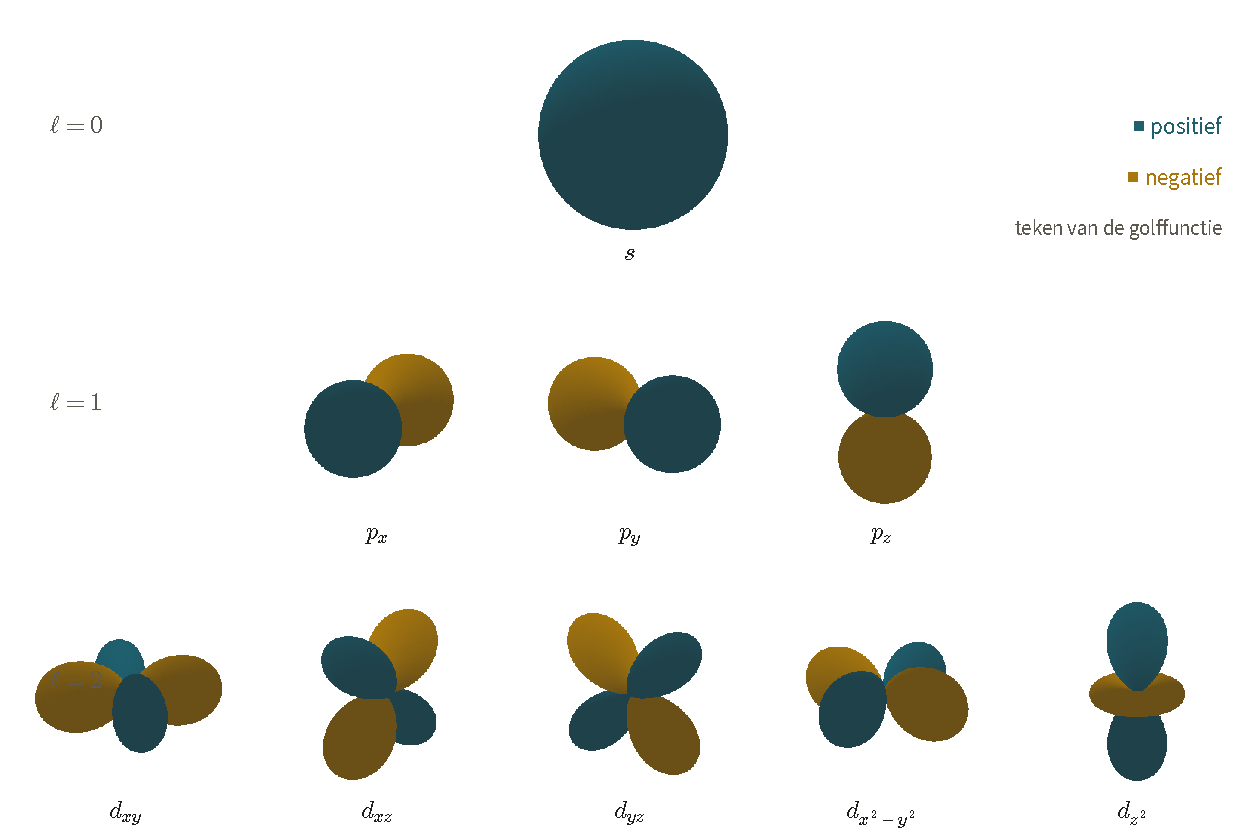
\includegraphics[width=0.62\linewidth]{Figuren/orbitalen}
    \caption{Typische waarschijnlijkheidsverdelingen van $s$-, $p$- en $d$-orbitalen.}
    \label{fig:orbitalen}
\end{figure}

Moleculen hebben naast elektronische ook gekwantiseerde rotatie- en vibratieniveaus (\S\ref{sec:moleculaire-beweging}). Daarom heeft elke stof een eigen ``vingerafdruk''-spectrum, de basis van de spectroscopie in kwaliteitscontrole en procesanalyse.

\section{Kwantumgetallen, het uitsluitingsprincipe en het periodiek systeem}

\subsection{Kwantumgetallen en orbitalen}

Elke oplossing van de Schr\"odingervergelijking voor een atoom is een orbitaal met een eigen energie en vorm. De chemische energie van een stof is dus de energie van de toegelaten toestanden waarin de elektronen zich bevinden; verandert die bezetting tijdens een reactie, dan verandert de energie. Elke elektrontoestand wordt volledig bepaald door vier \emph{kwantumgetallen}:
\begin{itemize}
\item het \emph{hoofdkwantumgetal} $n$ bepaalt vooral de energie en de gemiddelde afstand tot de kern;
\item het \emph{nevenkwantumgetal} $l$ bepaalt de vorm: $s$, $p$, $d$, $f$;
\item het \emph{magnetisch kwantumgetal} $m_l$ bepaalt de oriëntatie;
\item de \emph{spin} $m_s = \pm\tfrac{1}{2}$ is een kwantumeigenschap zonder klassiek equivalent (het elektron ``draait'' niet echt).
\end{itemize}

Net als een trillende snaar hebben orbitalen \emph{knopen}: oppervlakken waar $\psi = 0$ en de kans om het elektron te vinden dus nul is. Het $1s$-orbitaal heeft er geen. Elke extra knoop betekent een sterker gekromde golffunctie, dus een grotere kinetische energie in vergelijking~\eqref{eq:Schrodinger}. Meer knopen geeft daarom een hogere energie, net zoals een boventoon meer energie vraagt dan de grondtoon. Dezelfde logica keert terug bij rotatie en vibratie: meer structuur in de golffunctie betekent meer energie.

\subsection{Het uitsluitingsprincipe van Pauli}

De Schr\"odingervergelijking zegt welke orbitalen bestaan, niet hoe meerdere elektronen erover verdeeld worden. Dat legde Pauli in 1925 vast.

\begin{definitie}{Uitsluitingsprincipe van Pauli}
Twee elektronen in hetzelfde atoom kunnen nooit dezelfde vier kwantumgetallen hebben. Een orbitaal bevat dus hoogstens twee elektronen, met tegengestelde spin.
\end{definitie}

Dit is geen gevolg van de elektrostatische afstoting, maar een fundamentele eigenschap van elektronen (fermionen): hun gezamenlijke golffunctie zou bij twee identieke toestanden overal nul worden. Zodra een orbitaal vol is, moeten extra elektronen naar een hoger orbitaal. Zo ontstaat de gelaagde structuur van schillen en subschillen.

\subsection{Het periodiek systeem}

Elektronen bezetten eerst de orbitalen met de laagste energie (\emph{Aufbauprincipe}). Over orbitalen met gelijke energie, zoals de drie $2p$-orbitalen, verdelen ze zich eerst afzonderlijk met gelijke spin (\emph{regel van Hund}):
\begin{align*}
\text{C:}  &\quad 1s^2\,2s^2\,2p^1_x\, 2p^1_y &
\text{N:}  &\quad 1s^2\,2s^2\,2p^1_x\,2p^1_y\,2p^1_z &
\text{O:}  &\quad 1s^2\,2s^2\,2p^2_x\,2p^1_y\,2p^1_z
\end{align*}
De opvulvolgorde is $1s \to 2s \to 2p \to 3s \to 3p \to 4s \to 3d \to 4p \to 5s \to 4d \to \cdots$. Dat $4s$ vóór $3d$ komt, volgt uit de vorm van de golffuncties en de afscherming door de andere elektronen.

De buitenste elektronen, de \emph{valentie-elektronen}, bepalen grotendeels de chemie. Elementen met hetzelfde aantal valentie-elektronen gedragen zich gelijkaardig en staan in dezelfde groep. Het periodiek systeem is dus geen toevallige ordening: de Schr\"odingervergelijking, het uitsluitingsprincipe, het Aufbauprincipe en de regel van Hund verklaren samen de elektronenconfiguratie van elk element.

\section{Chemische bindingen}

\begin{casus}{waarom doet stikstof niets?}
Stikstof is het hoofdbestanddeel van de lucht, en toch reageert het bij kamertemperatuur met bijna niets. In hoofdstuk~\ref{ch:energie} zagen we dat de ammoniaksynthese \SI{200}{\bar}, \SI{450}{\celsius} en een katalysator nodig heeft. Wat maakt de stikstofmolecule zo stabiel?

\emph{Schat eerst zelf:} stikstof heeft vijf valentie-elektronen. Hoeveel bindingen verwacht je tussen twee stikstofatomen, en waarom?
\end{casus}

\subsection{Molecuulorbitalen}
\label{sec:molecuulorbitalen}

Brengt men twee atomen dicht bij elkaar, dan beïnvloeden hun golffuncties elkaar. Een binding ontstaat wanneer de gemeenschappelijke golffunctie een lagere energie heeft dan de gescheiden atomen. Een \emph{molecuulorbitaal} (MO) is een oplossing van de Schr\"odingervergelijking voor het volledige molecule. Bij benadering bouwt men het op als \emph{lineaire combinatie van atomaire orbitalen} (LCAO):
\begin{equation}
\psi_{\text{MO}} = c_1\,\psi_A \pm c_2\,\psi_B .
\end{equation}
\begin{itemize}
\item De \emph{bindende} combinatie ($+$, constructieve interferentie) versterkt $\psi$ tussen de kernen. De negatieve elektronendichtheid daar trekt beide kernen aan: lagere energie.
\item De \emph{antibindende} combinatie ($-$, aangeduid met $^*$) heeft een knoopvlak tussen de kernen. Zonder elektronendichtheid daar wint de kernafstoting: hogere energie.
\end{itemize}
Een \emph{$\sigma$-orbitaal} ontstaat door overlap langs de bindingsas en is rotatiesymmetrisch rond die as; een \emph{$\pi$-orbitaal} ontstaat door zijdelingse overlap van $p$-orbitalen. Een enkelvoudige binding is één $\sigma$-binding, een dubbele binding $\sigma + \pi$, een drievoudige $\sigma + 2\pi$. De sterkte volgt uit de \emph{bindingsorde}:
\begin{equation*}
\text{bindingsorde} = \frac{(\text{bindende elektronen}) - (\text{antibindende elektronen})}{2}.
\end{equation*}

\begin{figure}[htb]
    \centering
    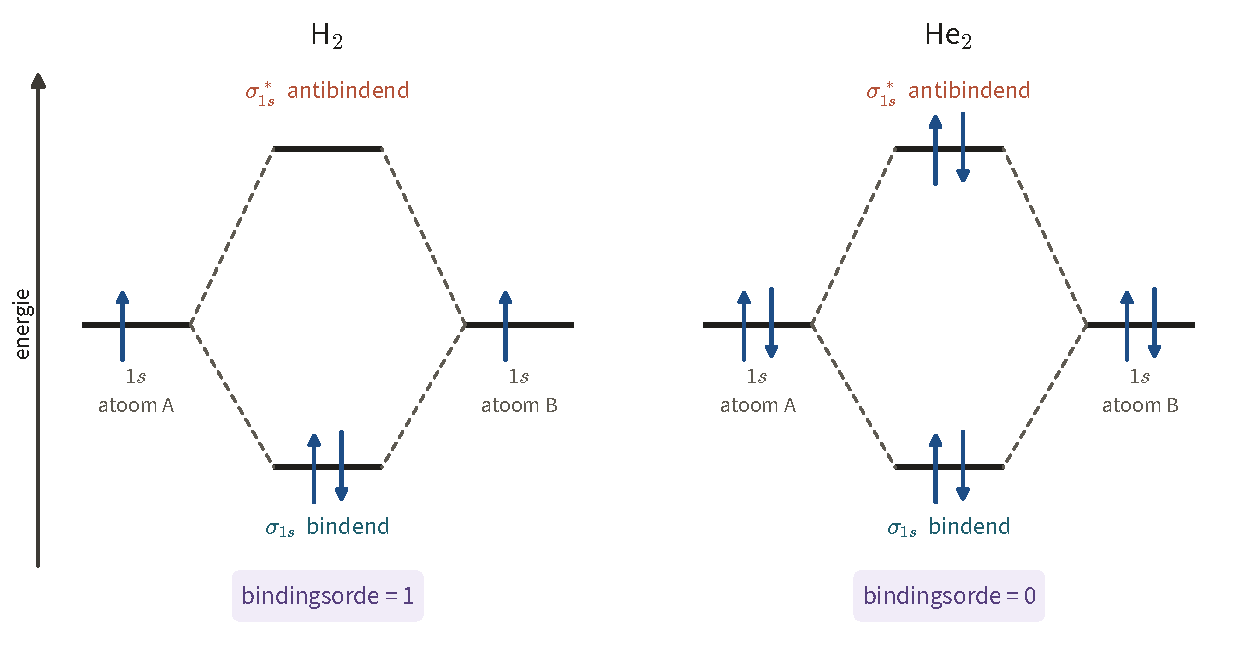
\includegraphics[width=0.62\linewidth]{Figuren/molecuulorbitalen}
    \caption{Molecuulorbitaaldiagram voor \ce{H2} (links) en \ce{He2} (rechts): de twee atomaire $1s$-orbitalen vormen een bindend $\sigma_{1s}$- en een antibindend $\sigma_{1s}^*$-orbitaal.}
    \label{fig:mo-H2}
\end{figure}

\begin{voorbeeld}{Waarom $\mathrm{H_2}$ bestaat en $\mathrm{He_2}$ niet}
In \ce{H2} bezetten de twee elektronen het bindende $\sigma_{1s}$ (figuur~\ref{fig:mo-H2}): bindingsorde $(2-0)/2 = 1$, een enkelvoudige binding. In \ce{He2} moeten de vier elektronen ook $\sigma_{1s}^*$ vullen: bindingsorde $(2-2)/2 = 0$. Bindende en antibindende bijdragen heffen elkaar op, en \ce{He2} bestaat niet als stabiele molecule.
\end{voorbeeld}

\subsection{Bindingsenergie, reactie-enthalpie en bindingslengte}
\label{sec:bindingslengte}

Bij de vorming van een binding komen de elektronen in een lagere energietoestand en wordt het verschil vrijgezet. De reactie-enthalpie is dus het verschil tussen de energie van de bindingen in reagentia en producten: zijn de nieuwe bindingen samen sterker, dan is de reactie exotherm.

Te ver uit elkaar overlappen de golffuncties niet genoeg; te dicht bij elkaar stoten de kernen elkaar af. Bij de \emph{bindingslengte} is de energie minimaal (figuur~\ref{fig:morse-h2}). Die lengte en de kromming van de put bepalen hoe een molecule roteert en vibreert.

\begin{figure}[htb]
    \centering
    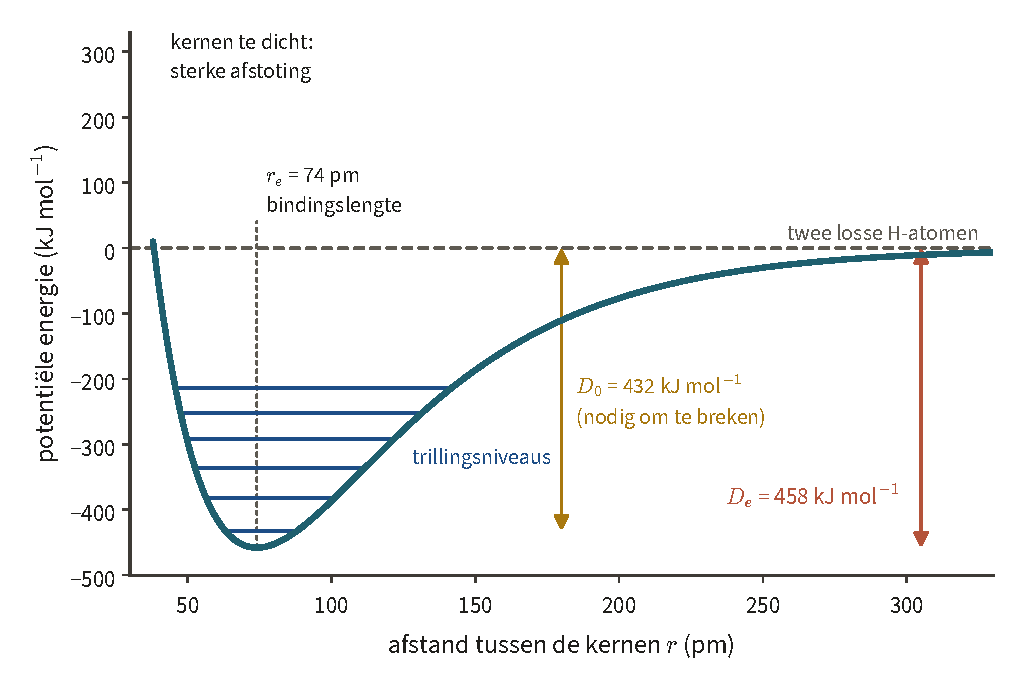
\includegraphics[width=0.62\linewidth]{Figuren/morse_h2}
    \caption{Potentiële energie van \ce{H2} tegen de kernafstand, met minimum bij $r_e = \SI{74}{\pico\metre}$. Door de trillingsenergie (horizontale niveaus) ligt de laagste toestand boven de bodem, zodat de bindingsenergie $D_0$ kleiner is dan de putdiepte $D_e$.}
    \label{fig:morse-h2}
\end{figure}

\begin{casusuitgewerkt}{waarom doet stikstof niets?}
Elk stikstofatoom brengt vijf valentie-elektronen mee ($2s^2\,2p^3$). Uit de acht atomaire orbitalen ($2s$ en drie $2p$ per atoom) ontstaan acht molecuulorbitalen (figuur~\ref{fig:mo-N2}). De tien valentie-elektronen vullen ze van onder naar boven: acht komen in bindende orbitalen ($\sigma_{2s}$, twee $\pi_{2p}$, $\sigma_{2p}$), twee in het antibindende $\sigma^*_{2s}$. De bindingsorde is
\[
\text{bindingsorde} = \frac{8 - 2}{2} = 3:
\]
een drievoudige binding, \'e\'en $\sigma$ en twee $\pi$. Ze is kort (\SI{110}{\pico\metre}) en zeer sterk: \SI{945}{\kilo\joule\per\mole}, bijna drie keer een C--C-binding. Om ze met licht te breken, is een foton van minstens $N_\mathrm{A}hc/\lambda = \SI{945}{\kilo\joule\per\mole}$ nodig, dus $\lambda < \SI{127}{\nano\metre}$: ver ultraviolet, dat de onderste atmosfeer niet bereikt. Bovendien ligt het hoogst bezette orbitaal laag en het laagste lege orbitaal ($\pi^*_{2p}$) hoog, zodat de molecule elektronen moeilijk afgeeft of opneemt. Daarom heeft de ammoniaksynthese een katalysator nodig die de binding helpt verzwakken (hoofdstukken~\ref{ch:grensvlakken} en~\ref{ch:kinetiek}).

\emph{Volgende vraag.} Een binding is geen starre staaf: ze kan trillen, zoals de niveaus in figuur~\ref{fig:morse-h2} tonen. Zowel \ce{N2} als \ce{CO2} heeft sterke bindingen die trillen. Waarom absorbeert dan enkel CO$_2$ infrarood?
\end{casusuitgewerkt}

\begin{figure}[htb]
    \centering
    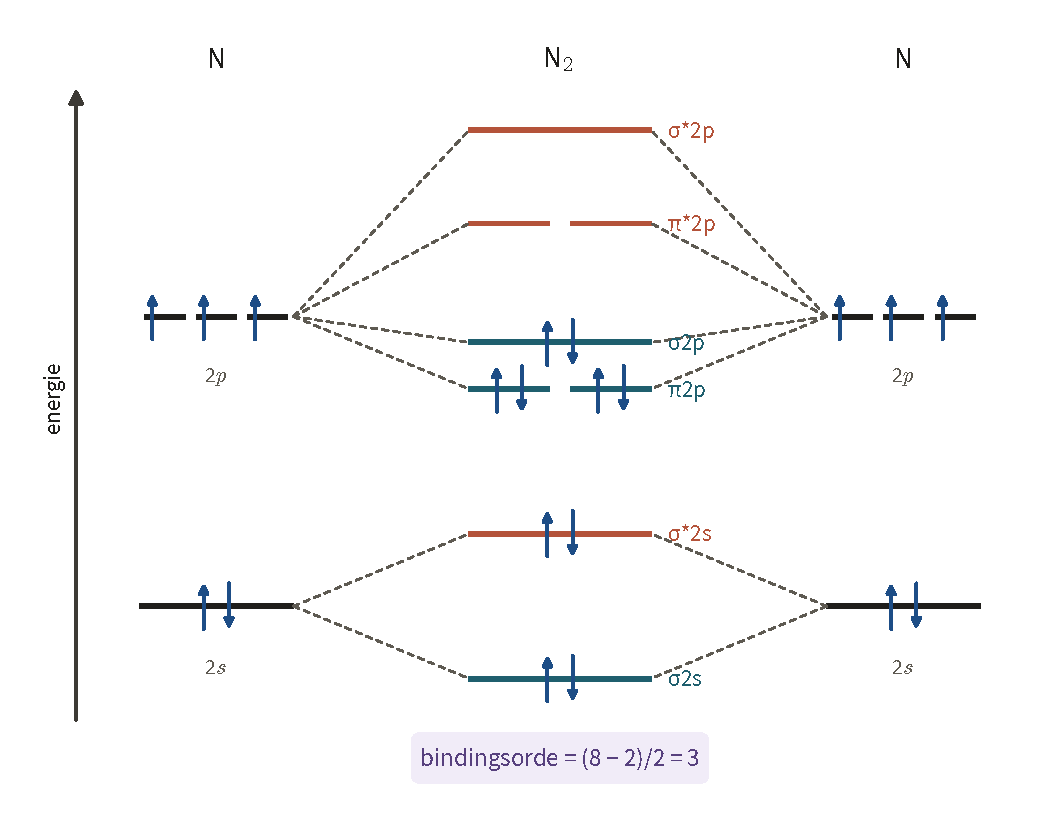
\includegraphics[width=0.7\linewidth]{Figuren/mo_stikstof}
    \caption{Molecuulorbitaaldiagram van \ce{N2} (enkel de valentie-elektronen). Acht elektronen in bindende orbitalen, twee in een antibindend orbitaal: een drievoudige binding. Bij \ce{N2} ligt $\sigma_{2p}$ net boven $\pi_{2p}$; bij \ce{O2} en \ce{F2} is die volgorde omgekeerd.}
    \label{fig:mo-N2}
\end{figure}

\section{Moleculaire beweging en moleculaire spectra}
\label{sec:moleculaire-beweging}

\begin{casus}{CO$_2$ tegenover stikstof}
De drievoudige binding van \ce{N2} trilt, net als de bindingen in CO$_2$. Toch laat stikstof het infrarood van de aarde volledig door, terwijl CO$_2$ het bij \SI{4.3}{} en \SI{15}{\micro\metre} absorbeert. Wat bepaalt of een molecule infrarood licht kan opnemen?

\emph{Schat eerst zelf:} licht is een elektrisch veld dat heen en weer schommelt. Waaraan kan zo'n veld ``trekken'' in een molecule? Is er een verschil tussen \ce{N2}, waarin beide atomen gelijk zijn, en CO$_2$?
\end{casus}

Een molecule kan als geheel door de ruimte bewegen (\emph{translatie}), rond zijn zwaartepunt tollen (\emph{rotatie}) en zijn kernen laten trillen rond de evenwichtsafstand (\emph{vibratie}). Ook die bewegingen volgen de Schr\"odingervergelijking en zijn dus gekwantiseerd, elk met een eigen kwantumgetal. Zo kan een molecule energie opnemen zonder dat een elektron van toestand verandert. Dit verklaart de warmtecapaciteit en vormt de basis van infrarood- en microgolfspectroscopie.

\subsection{Translatie: het deeltje in een doos}
\label{sec:translatie}

De translatie van een molecule in een vat is het deeltje in een doos van \S~\ref{sec:discrete-energieniveaus}, met translationeel kwantumgetal $n_{\mathrm{trans}}$:
\begin{equation}
\boxed{
E_{n_{\mathrm{trans}}} = \frac{n_{\mathrm{trans}}^2 h^2}{8mL^2}, \qquad n_{\mathrm{trans}}=1,2,3,\ldots
}
\end{equation}

\begin{voorbeeld}{Translatieniveaus van \ce{N2} in een vat}
Eén \ce{N2}-molecule ($m=\SI{4.652e-26}{kg}$) in een vat met $L=\SI{0.10}{m}$:
\[
E_1 = \frac{(6.626\times10^{-34})^2}{8(4.652\times10^{-26})(0.10)^2} = \SI{1.18e-40}{J}, \qquad \Delta E_{1\to2} = 3E_1 = \SI{3.54e-40}{J}.
\]
Bij \SI{298}{K} is $k_BT = \SI{4.12e-21}{J}$, zodat $\Delta E/k_BT \approx 10^{-19}$. De translatieniveaus liggen zo dicht bij elkaar dat ze voor alle praktische doeleinden continu zijn.
\end{voorbeeld}

\subsection{Rotatie: de starre rotator}
\label{sec:rotatie}

Een tweeatomige molecule roteert rond een as loodrecht op de binding. In het model van de \emph{starre rotator} zijn twee massa's verbonden door een staaf met de bindingslengte $r$. Met de \emph{gereduceerde massa} $\mu = m_1 m_2/(m_1+m_2)$ en het traagheidsmoment $I = \mu r^2$ levert de Schr\"odingervergelijking het \emph{rotationeel kwantumgetal} $J$:
\begin{equation}
\boxed{
E_J = J(J+1)\frac{\hbar^2}{2I}, \qquad J=0,1,2,\ldots
}
\end{equation}
Elk niveau is $(2J+1)$-voudig \emph{ontaard}: er bestaan $2J+1$ oriëntaties van de rotatie-as met exact dezelfde energie, zoals de drie $p$-orbitalen dezelfde energie hebben.

\begin{voorbeeld}{Rotatieniveaus van HCl}
HCl heeft $r=\SI{127.5}{pm}$, $m_H=\SI{1.008}{u}$ en $m_{Cl}=\SI{34.97}{u}$ ($\SI{1}{u}=\SI{1.6605e-27}{kg}$). Dan is $\mu = \SI{1.628e-27}{kg}$ en $I = \mu r^2 = \SI{2.646e-47}{kg\,m^2}$, zodat
\[
\frac{\hbar^2}{2I} = \frac{(1.0546\times10^{-34})^2}{2(2.646\times10^{-47})} = \SI{2.10e-22}{J}, \qquad \Delta E_{0\to1} = \SI{4.20e-22}{J} \approx 0.10\,k_BT.
\]
Rotatieniveaus liggen dicht genoeg om bij kamertemperatuur ruim bezet te zijn. Overgangen ertussen liggen in het microgolfgebied.
\end{voorbeeld}

\subsection{Vibratie: de harmonische oscillator}
\label{sec:vibratie}

Voor kleine uitwijkingen rond de bindingslengte gedraagt een binding zich als een veer met veerconstante $k$: de \emph{harmonische oscillator}. Het \emph{vibrationeel kwantumgetal} $v$ geeft
\begin{equation}
\boxed{
E_v = \left(v+\frac{1}{2}\right)h\nu, \qquad \nu = \frac{1}{2\pi}\sqrt{\frac{k}{\mu}}, \qquad v=0,1,2,\ldots
}
\end{equation}
Zelfs in de grondtoestand is de energie niet nul maar $\tfrac{1}{2}h\nu$, de \emph{nulpuntsenergie}: een binding trilt altijd, ook bij \SI{0}{K}.

\begin{voorbeeld}{Vibratie van CO}
CO heeft $k=\SI{1902}{N/m}$ en $\mu = \SI{1.139e-26}{kg}$. Dan is
\[
\nu = \frac{1}{2\pi}\sqrt{\frac{1902}{1.139\times10^{-26}}} = \SI{6.50e13}{Hz}, \qquad \tilde\nu = \nu/c = \SI{2168}{cm^{-1}},
\]
dicht bij de gemeten infraroodabsorptie (\SI{2143}{cm^{-1}}). De stap tussen niveaus is $h\nu = \SI{4.31e-20}{J} \approx 10.5\,k_BT$. Slechts één op de $\mathrm{e}^{10.5} \approx 37\,000$ moleculen zit bij kamertemperatuur in $v=1$: vibratie is ``bevroren''. De nulpuntsenergie bedraagt $\tfrac{1}{2}h\nu = \SI{12.97}{kJ/mol}$.
\end{voorbeeld}

De energiestappen van de verschillende bewegingen liggen vele grootteordes uit elkaar:

\begin{center}
\begin{tabular}{lccc}
\toprule
Beweging & Kwantumgetal & Typische $\Delta E$ & Spectraal gebied \\
\midrule
Translatie & $n_{\mathrm{trans}}$ & $\sim 10^{-40}~\mathrm{J}$ ($\ll k_BT$) & quasi-continu \\
Rotatie & $J$ & $\sim 10^{-22}$--$10^{-21}~\mathrm{J}$ ($\sim k_BT$) & microgolf \\
Vibratie & $v$ & $\sim 10^{-20}~\mathrm{J}$ ($\gg k_BT$) & infrarood \\
Elektronisch & $n,l,m_l,m_s$ & $\sim 10^{-19}$--$10^{-18}~\mathrm{J}$ & zichtbaar/UV \\
\bottomrule
\end{tabular}
\end{center}

Bij stijgende temperatuur worden de bewegingen daarom ``na elkaar'' geactiveerd: bij kamertemperatuur zijn translatie en rotatie volledig actief, vibratie nauwelijks, en elektronische aanslag niet.

\subsection{Moleculaire spectra}
\label{sec:moleculaire-spectra}

Elke overgang tussen twee niveaus absorbeert of zendt een foton uit met $\Delta E = h\nu$. Omdat de energieschalen zo verschillen, vallen de spectra in gescheiden gebieden:
\begin{itemize}
\item \textbf{Rotatiespectra} (microgolf, selectieregel $\Delta J=\pm1$) vereisen een permanent dipoolmoment. \ce{N2} en \ce{O2} hebben dat niet en zijn microgolf-inactief.
\item \textbf{Vibratiespectra} (infrarood, $\Delta v=\pm1$) vereisen dat het dipoolmoment \emph{verandert} tijdens de trilling; waarom, zie je in de casus hieronder. Elke functionele groep heeft een eigen IR-band, wat infraroodspectroscopie het standaardinstrument voor procesanalyse maakt.
\item \textbf{Elektronische spectra} (zichtbaar en UV), bijvoorbeeld een $\pi\to\pi^*$-overgang tussen het hoogst bezette (HOMO) en laagst onbezette molecuulorbitaal (LUMO), verklaren kleur: een stof die een bepaalde golflengte absorbeert, toont de complementaire kleur. UV-Vis-spectroscopie meet zo concentraties via de wet van Lambert--Beer.
\end{itemize}

\begin{casusuitgewerkt}{CO$_2$ tegenover stikstof}
\emph{Stap 1: wat trekt het licht?} Het elektrisch veld van een lichtgolf duwt positieve en negatieve ladingen in tegengestelde richting. Het kan dus enkel energie overdragen aan een trilling als die trilling de ladingsverdeling, het \emph{dipoolmoment}, heen en weer laat schommelen in hetzelfde ritme.

\emph{Stap 2: stikstof.} In \ce{N2} zijn beide atomen gelijk; de elektronen zitten altijd symmetrisch verdeeld. Hoe ver de atomen ook uit elkaar gaan, het dipoolmoment blijft nul. De trilling bestaat (bij \SI{2330}{\per\centi\metre}, ongeveer \SI{4.3}{\micro\metre}), maar het licht kan er niet aan trekken: \ce{N2} is IR-inactief. Hetzelfde geldt voor \ce{O2}.

\emph{Stap 3: CO$_2$.} Een lineaire molecule met drie atomen heeft vier trillingen (figuur~\ref{fig:trillingen-co2}). Zuurstof trekt elektronen sterker aan dan koolstof, zodat elke C=O-binding een eigen dipool heeft. In de rechte molecule heffen beide dipolen elkaar op.
\begin{itemize}
\item Bij de \emph{symmetrische strek} bewegen beide zuurstofatomen tegelijk naar buiten: de dipolen blijven elkaar opheffen. IR-inactief.
\item Bij de \emph{asymmetrische strek} wordt de ene binding langer en de andere korter: er ontstaat een schommelende dipool langs de as. IR-actief bij \SI{2349}{\per\centi\metre}, of $\lambda = 1/\tilde\nu = \SI{4.26}{\micro\metre}$: de lijn van de CO$_2$-meter.
\item Bij de \emph{buiging} (in twee loodrechte richtingen, dus twee keer) knikt de molecule: er ontstaat een dipool loodrecht op de as. IR-actief bij \SI{667}{\per\centi\metre}, of \SI{15.0}{\micro\metre}.
\end{itemize}

\emph{Stap 4: waarom de buiging het klimaat bepaalt.} De buiging absorbeert bij \SI{15}{\micro\metre}, vlak naast het maximum van de straling van de aarde (\SI{10}{\micro\metre}, figuur~\ref{fig:zon-aarde}). De asymmetrische strek bij \SI{4.3}{\micro\metre} valt in een gebied waar de aarde nauwelijks straalt; ze is ideaal voor een meettoestel, maar speelt in het klimaat een kleine rol. De energie van een buigingsfoton is $N_\mathrm{A}hc\tilde\nu = \SI{8.0}{\kilo\joule\per\mole}$, slechts drie keer $RT$ bij \SI{15}{\celsius}.

\emph{Volgende vraag.} Bij \SI{15}{\celsius} is $RT = \SI{2.4}{\kilo\joule\per\mole}$, niet zo veel kleiner dan de \SI{8.0}{\kilo\joule\per\mole} van de buiging. Trillen sommige CO$_2$-moleculen dan al vanzelf, zonder licht? En wat betekent dat voor de warmte die het gas opneemt?
\end{casusuitgewerkt}

\begin{figure}[htb]
    \centering
    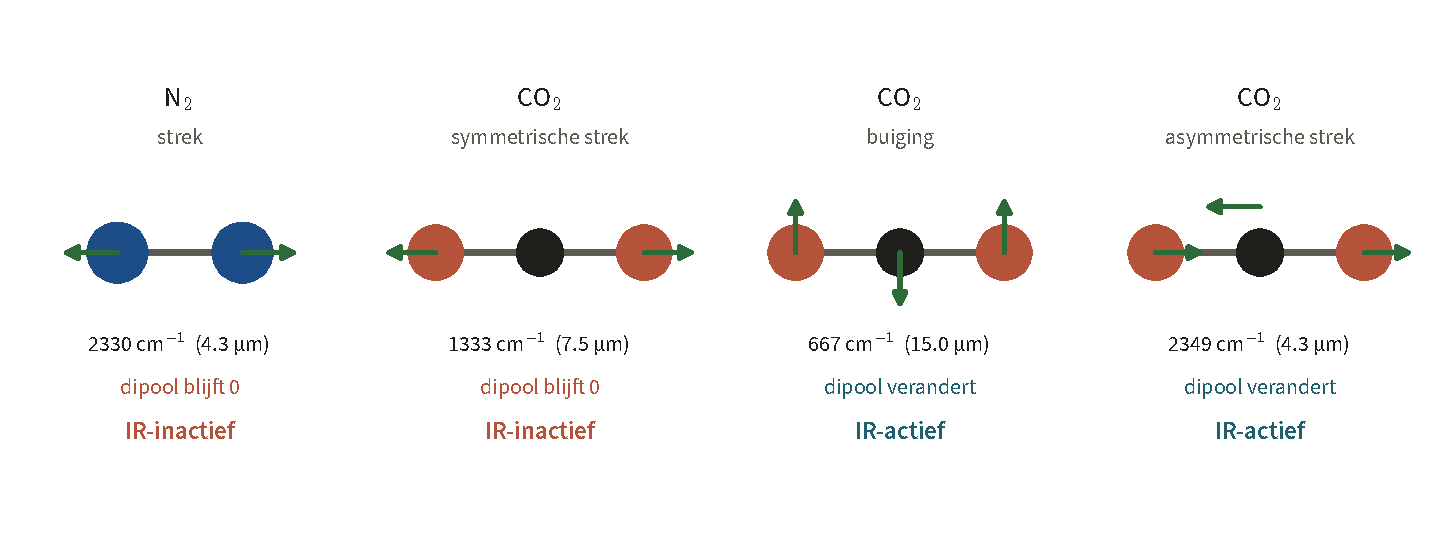
\includegraphics[width=\linewidth]{Figuren/trillingen_co2}
    \caption{De trilling van \ce{N2} en de trillingen van CO$_2$ (de buiging komt twee keer voor, in twee loodrechte vlakken). Enkel trillingen die het dipoolmoment doen veranderen, absorberen infrarood. Golfgetallen: NIST; de symmetrische strek van CO$_2$ is een gemiddelde van twee gekoppelde banden (1285 en \SI{1388}{\per\centi\metre}).}
    \label{fig:trillingen-co2}
\end{figure}

\section{Van kwantumtoestanden naar thermodynamica}
\label{sec:kwantum-thermo}

\begin{casus}{waarom neemt CO$_2$ meer warmte op?}
Bij \SI{25}{\celsius} is $C_{p,\mathrm{m}} = \SI{29.1}{\joule\per\mole\per\kelvin}$ voor stikstof en \SI{37.1}{\joule\per\mole\per\kelvin} voor CO$_2$ (tabel~\ref{tab:cp_coeff}). Beide zijn lineaire moleculen die even vrij bewegen en draaien. Waar komt het verschil van \SI{8}{\joule\per\mole\per\kelvin} vandaan? En hoeveel CO$_2$-moleculen in de atmosfeer trillen al bij \SI{15}{\celsius}?

\emph{Schat eerst zelf:} welke beweging heeft CO$_2$ die stikstof bij kamertemperatuur niet kan aanslaan? Kijk naar de golfgetallen in figuur~\ref{fig:trillingen-co2}.
\end{casus}

\subsection{De Boltzmannverdeling}
\label{sec:boltzmannverdeling}

Een mol gas bevat $6\times10^{23}$ moleculen. De vraag is dus niet in welk niveau \emph{één} molecule zit, maar hoeveel moleculen gemiddeld in elk niveau zitten. In thermisch evenwicht geldt voor twee niveaus met energieverschil $\Delta E = E_i - E_j$ de \emph{Boltzmannverdeling}:
\begin{equation}
\boxed{\frac{N_i}{N_j} = \frac{g_i}{g_j}\,\exp\!\left(-\frac{\Delta E}{k_\mathrm{B}T}\right)}
\label{eq:boltzmann}
\end{equation}
met $k_\mathrm{B} = \SI{1.381e-23}{\joule\per\kelvin}$ en $g_i$ de ontaarding (voor vibratieniveaus $g = 1$). Per mol schrijf je $\Delta E_\mathrm{m}/RT$, want $R = N_\mathrm{A}k_\mathrm{B}$. We leiden de verdeling hier niet af, maar de betekenis is eenvoudig: $k_\mathrm{B}T$ is de typische thermische energie die een molecule bij botsingen uitwisselt ($RT = \SI{2.48}{\kilo\joule\per\mole}$ bij \SI{298}{\kelvin}).
\begin{itemize}
\item $\Delta E \ll k_\mathrm{B}T$: beide niveaus zijn bijna even sterk bezet; de beweging gedraagt zich klassiek (translatie, rotatie).
\item $\Delta E \gg k_\mathrm{B}T$: het hogere niveau is vrijwel leeg; de beweging is ``bevroren'' (vibratie bij kamertemperatuur).
\item Een hogere temperatuur bevolkt hogere niveaus, maar het laagste blijft altijd het sterkst bezet (bij gelijke $g$).
\end{itemize}

\begin{voorbeeld}{Vibrerende stikstof in een vlam}
De vibratie van \ce{N2} ($\tilde\nu = \SI{2330}{\per\centi\metre}$) heeft $\Delta E = hc\tilde\nu = \SI{4.63e-20}{\joule}$. Bij \SI{300}{\kelvin} is $\Delta E/k_\mathrm{B}T = 11.2$ en $N_1/N_0 = 1.4\times10^{-5}$. Bij \SI{2000}{\kelvin} is $\Delta E/k_\mathrm{B}T = 1.68$ en $N_1/N_0 = 0.19$: bijna één op vijf moleculen vibreert. Daarom stijgt $C_p$ van stikstof van \SI{29.1}{} naar \SI{36}{\joule\per\mole\per\kelvin}, en moesten we voor de vlamtemperatuur in hoofdstuk~\ref{ch:energie} met een temperatuurafhankelijke $C_p$ rekenen.
\end{voorbeeld}

\begin{toepassing}{De luchtdruk op de berg}
De Boltzmannverdeling geldt voor elke vorm van energie, ook voor de potentiële energie $Mgh$ per mol in het zwaartekrachtveld. De druk daalt daarom exponentieel met de hoogte:
\begin{equation}
p(h) = p_0 \exp\!\left(-\frac{Mgh}{RT}\right).
\end{equation}
Met $M = \SI{0.029}{\kilo\gram\per\mole}$ en $T \approx \SI{273}{\kelvin}$ daalt de druk met een factor $\mathrm{e}$ per \SI{8}{\kilo\metre}. Op de Mont Blanc (\SI{4808}{\metre}) is de druk ongeveer \SI{0.55}{\bar}, op de Everest (\SI{8849}{\metre}) \SI{0.33}{\bar}. Water kookt daar al bij ongeveer \SI{70}{\celsius} (hoofdstuk~\ref{ch:niet-reagerend}).
\end{toepassing}

\subsection{Warmtecapaciteit}

In hoofdstuk~\ref{ch:energie} was $C_{V,m}$ een experimenteel gegeven: ongeveer $\tfrac{3}{2}R$ voor een eenatomig gas en $\tfrac{5}{2}R$ voor een tweeatomig gas bij kamertemperatuur. Nu kunnen we dat verklaren. Volgens de \emph{equipartitiestelling} draagt elke bewegingsrichting die klassiek toegankelijk is ($\Delta E \ll k_BT$) $\tfrac{1}{2}R$ per mol bij.
\begin{itemize}
\item Een eenatomig gas transleert in drie richtingen: $C_{V,m}=\tfrac{3}{2}R$.
\item Een lineair tweeatomig gas roteert bovendien rond twee assen (rotatie rond de bindingsas telt niet): $C_{V,m}=\tfrac{5}{2}R = \SI{20.8}{J/(mol\,K)}$. Voor CO is de gemeten waarde \SI{20.2}{J/(mol\,K)}.
\item Vibratie draagt pas bij als $k_BT$ vergelijkbaar wordt met $h\nu$, en dan met $R$ per trilling (kinetische plus potentiële energie). $C_{V,m}$ stijgt daardoor geleidelijk naar $\tfrac{7}{2}R$.
\end{itemize}

Hoe groot die bijdrage van een trilling precies is, volgt uit de Boltzmannverdeling. We geven het resultaat zonder afleiding; het hangt enkel af van de verhouding $x = h\nu/k_\mathrm{B}T$:
\begin{equation}
C_{V,\mathrm{vib}} = R\,\frac{x^2\,\mathrm{e}^{x}}{(\mathrm{e}^{x}-1)^2}, \qquad x = \frac{h\nu}{k_\mathrm{B}T} = \frac{hc\tilde\nu}{k_\mathrm{B}T}.
\label{eq:cv-vib}
\end{equation}
Bij lage temperatuur ($x \gg 1$) is de bijdrage nul, bij hoge temperatuur ($x \ll 1$) nadert ze $R$. Figuur~\ref{fig:cp-co2-n2} toont dat dit eenvoudige model de gemeten warmtecapaciteit van \ce{N2} en CO$_2$ over het hele temperatuurbereik volgt.

\begin{figure}[htb]
    \centering
    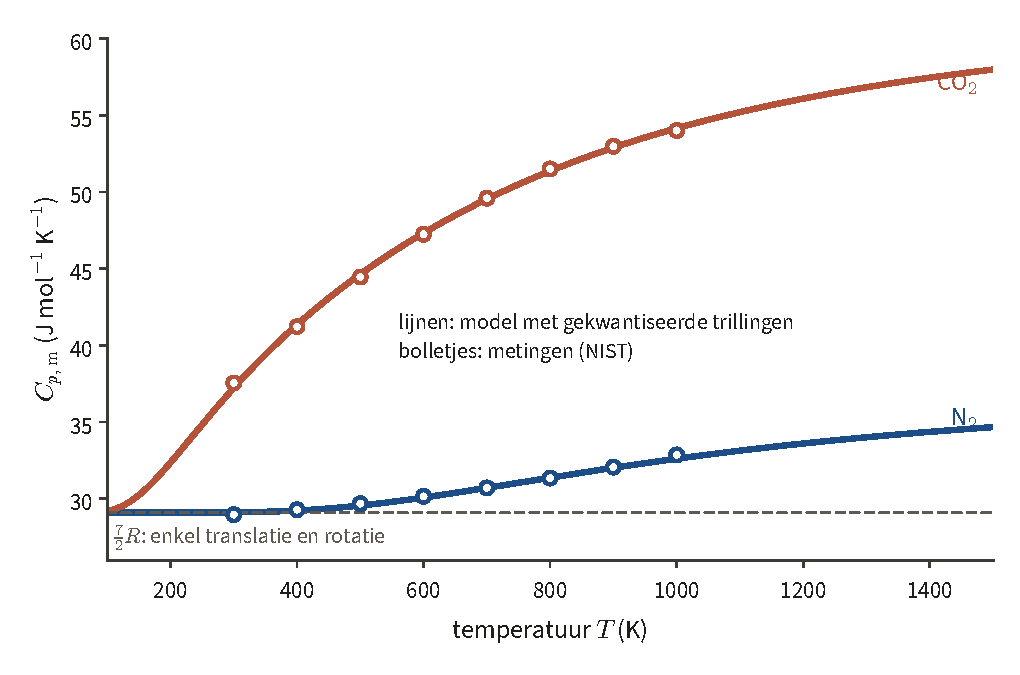
\includegraphics[width=0.7\linewidth]{Figuren/cp_co2_n2}
    \caption{Warmtecapaciteit van \ce{N2} en CO$_2$. Lijnen: $\tfrac72R$ plus de bijdrage~\eqref{eq:cv-vib} van elke trilling (golfgetallen uit figuur~\ref{fig:trillingen-co2}). Bolletjes: correlaties uit tabel~\ref{tab:cp_coeff} (NIST).}
    \label{fig:cp-co2-n2}
\end{figure}

\begin{casusuitgewerkt}{waarom neemt CO$_2$ meer warmte op?}
\emph{Stap 1: hoeveel CO$_2$ trilt?} Voor de buiging ($\tilde\nu = \SI{667}{\per\centi\metre}$) is bij \SI{288}{\kelvin}
\[
x = \frac{hc\tilde\nu}{k_\mathrm{B}T} = \frac{(6.626\times10^{-34})(2.998\times10^{10})(667)}{(1.381\times10^{-23})(288)} = 3.33,
\qquad
\frac{N_1}{N_0} = 2\,\mathrm{e}^{-3.33} = 0.071.
\]
De factor 2 is de ontaarding: de molecule kan in twee loodrechte vlakken buigen. Zeven procent van de CO$_2$-moleculen buigt dus al door de botsingen met andere moleculen. Zo'n trillende molecule kan haar energie als infraroodfoton uitzenden, in elke richting, ook terug naar de aarde. Daarom houdt CO$_2$ de warmte vast: het absorbeert de straling van de aarde, geeft de energie bij botsingen door aan de lucht, en straalt een deel terug naar beneden. Voor de asymmetrische strek is $x = 11.7$ en trilt slechts \'e\'en molecule op honderdduizend.

\emph{Stap 2: de warmtecapaciteit.} Bij \SI{298}{\kelvin} geeft vergelijking~\eqref{eq:cv-vib} per trilling:
\begin{center}
\begin{tabular}{lccc}
\toprule
Trilling & $\tilde\nu$ (\si{\per\centi\metre}) & $x$ & $C_{V,\mathrm{vib}}$ (\si{\joule\per\mole\per\kelvin}) \\
\midrule
CO$_2$ buiging ($2\times$) & 667 & 3.22 & $2 \times 3.74 = 7.48$ \\
CO$_2$ symmetrische strek & 1333 & 6.43 & 0.56 \\
CO$_2$ asymmetrische strek & 2349 & 11.3 & 0.01 \\
\ce{N2} strek & 2330 & 11.2 & 0.01 \\
\bottomrule
\end{tabular}
\end{center}
Translatie en rotatie geven samen $\tfrac52R$, en $C_p = C_V + R$ (hoofdstuk~\ref{ch:energie}), dus $\tfrac72R = \SI{29.10}{\joule\per\mole\per\kelvin}$ voor elke lineaire molecule. Daarbij komt de bijdrage van de trillingen:
\begin{align*}
C_{p,\mathrm{m}}(\ce{N2}) &= 29.10 + 0.01 = \SI{29.1}{\joule\per\mole\per\kelvin},\\
C_{p,\mathrm{m}}(\ce{CO2}) &= 29.10 + 7.48 + 0.56 + 0.01 = \SI{37.2}{\joule\per\mole\per\kelvin}.
\end{align*}
Gemeten: 29.1 en \SI{37.1}{\joule\per\mole\per\kelvin}. Het hele verschil komt van de zachte buiging van CO$_2$, die als enige trilling al bij kamertemperatuur energie opneemt. Bij hogere temperatuur komen ook de andere trillingen vrij, en daarom stijgt $C_p$ met $T$ (figuur~\ref{fig:cp-co2-n2}): de veelterm uit tabel~\ref{tab:cp_coeff} is geen toevallige curve-fit, maar een gevolg van gekwantiseerde trillingsniveaus.
\end{casusuitgewerkt}

\subsection{Activeringsenergie en overgangstoestand}
\label{sec:activeringsenergie-kwantum}

Tijdens een reactie verdwijnen oude bindingen niet op hetzelfde ogenblik dat nieuwe ontstaan. Het systeem passeert tussentoestanden waarvan sommige een hogere energie hebben dan zowel reagentia als producten. De minimale energie om die \emph{overgangstoestand} te bereiken, is de \emph{activeringsenergie}. Ze verklaart waarom een reactie thermodynamisch gunstig maar toch traag kan zijn: de thermodynamica bepaalt de eindtoestand, de kinetiek hoe snel die bereikt wordt. Enkel moleculen die toevallig genoeg energie bezitten, halen de overgangstoestand. Hoeveel dat er zijn, zegt opnieuw de Boltzmannverdeling.

\subsection{Waarom reacties sneller gaan bij hogere temperatuur}

Een reactie verloopt enkel als botsende moleculen minstens de activeringsenergie $E_\mathrm{a}$ bezitten. Die fractie volgt uit dezelfde Boltzmannfactor, $\exp(-E_\mathrm{a}/RT)$. Voor $E_\mathrm{a} = \SI{50}{\kilo\joule\per\mole}$ is ze bij \SI{35}{\celsius} een factor
\[
\exp\!\left[\frac{50\,000}{8.314}\left(\frac{1}{298.15} - \frac{1}{308.15}\right)\right] = 1.9
\]
groter dan bij \SI{25}{\celsius}. Dat is de oorsprong van de vuistregel ``twee keer sneller per \SI{10}{\celsius}'' en van de wet van Arrhenius (hoofdstuk~\ref{ch:kinetiek}). Een koelkast vertraagt bederfreacties volgens hetzelfde principe.

\section{Het broeikaseffect opnieuw bekeken}

Met de begrippen uit dit hoofdstuk kan je de vragen uit het begin beantwoorden:
\begin{itemize}
\item \emph{Zon en aarde} (\S\ref{sec:licht-pakketjes}): de kleur van de straling volgt uit de temperatuur (wet van Wien). Zonlicht heeft fotonen van zo'n \SI{240}{\kilo\joule\per\mole}, het infrarood van de aarde slechts \SI{12}{\kilo\joule\per\mole}: genoeg om moleculen te laten trillen, niet om bindingen te breken. Zonder broeikasgassen zou de aarde \SI{-18}{\celsius} zijn.
\item \emph{Scherpe lijnen} (\S\ref{sec:lijnenspectra}): een molecule absorbeert enkel fotonen met $h\nu = \Delta E$ tussen twee toegelaten niveaus. Bij \SI{4.26}{\micro\metre} hoort \SI{28}{\kilo\joule\per\mole}, te weinig voor een elektronische overgang.
\item \emph{Stikstof} (\S\ref{sec:molecuulorbitalen}): een drievoudige binding met bindingsorde 3 en \SI{945}{\kilo\joule\per\mole}; daarom is stikstof zo inert en heeft de ammoniaksynthese een katalysator nodig.
\item \emph{CO$_2$ tegenover stikstof} (\S\ref{sec:moleculaire-beweging}): enkel trillingen die het dipoolmoment doen veranderen, absorberen infrarood. \ce{N2} en \ce{O2} hebben er geen, CO$_2$ heeft er twee: de buiging bij \SI{15}{\micro\metre} (klimaat) en de asymmetrische strek bij \SI{4.26}{\micro\metre} (CO$_2$-meter).
\item \emph{Warmtecapaciteit} (\S\ref{sec:kwantum-thermo}): de zachte buiging van CO$_2$ wordt al bij kamertemperatuur aangeslagen; ze verklaart \SI{8}{\joule\per\mole\per\kelvin} extra warmtecapaciteit en de \SI{7}{\percent} trillende CO$_2$-moleculen die infrarood terugstralen.
\end{itemize}
Dezelfde redeneringen gelden voor elk molecule: waterdamp en methaan zijn broeikasgassen om dezelfde reden als CO$_2$, en de infraroodbanden van functionele groepen maken infraroodspectroscopie tot een standaardinstrument in labo en procescontrole.

Eén vraag blijft open: waarom verlopen sommige processen spontaan in één richting, ook als de energie geen uitsluitsel geeft? Het antwoord ligt in het \emph{aantal manieren} waarop energie en moleculen over de toestanden verdeeld kunnen worden: de entropie van hoofdstuk~\ref{ch:spontaniteit}.

\section{Oefeningen}

% Oefeningen bij dit hoofdstuk (ingevoegd achteraan het hoofdstuk met \input).
% Een oefening:  \begin{oefening} ... \end{oefening}   (boek en website)
% De oplossing:  \begin{oplossing} ... \end{oplossing}       (enkel website, dichtgeklapt)

Constanten: $h = \SI{6.626e-34}{\joule\second}$, $c = \SI{2.998e8}{\metre\per\second}$, $k_B = \SI{1.381e-23}{\joule\per\kelvin}$, $m_e = \SI{9.109e-31}{\kilogram}$, $\SI{1}{\electronvolt} = \SI{1.602e-19}{\joule}$, $1\,\mathrm{u} = \SI{1.6605e-27}{\kilogram}$, $N_A = \SI{6.022e23}{\per\mole}$.

\begin{oefening}
Cesium heeft een elektronenbindingsenergie (werkfunctie) van \(1.95\,\mathrm{eV}\).

\begin{enumerate}
\item[(a)]
  Bereken de minimale frequentie en golflengte van licht die nodig is om elektronen uit een cesiumoppervlak los te slaan.
\item[(b)]
  Wordt zichtbaar licht (ca. \(400\)--\(700\,\mathrm{nm}\)) hiervoor gebruikt? Of eerder UV?
\item[(c)]
  Bereken de maximale kinetische energie van de losgeslagen elektronen wanneer cesium wordt belicht met licht van \(\lambda = 400\,\mathrm{nm}\).
\end{enumerate}

\emph{Hint:} gebruik \(E_{\text{foton}} = h\nu = hc/\lambda\) en \(1~\mathrm{eV} = 1.602\times10^{-19}\,\mathrm{J}\).
\end{oefening}
\begin{oplossing}
\textbf{Resultaat:} (a) \(\nu_0\) = \textbf{4.71\ensuremath{\cdot{}}10\ensuremath{^{14}} Hz}, \(\lambda_0\) = \textbf{636 nm}. (b) Zichtbaar licht volstaat (alles onder 636 nm). (c) \(E_{k,\max}\) = \textbf{1.15 eV} (1.84\ensuremath{\cdot{}}10\ensuremath{^{-19}} J).

\textbf{(a)} De drempelfrequentie volgt uit \(h\nu_0 = \phi\):

\[
\nu_0 = \frac{(1.95)(1.602\times10^{-19})}{6.626\times10^{-34}} = 4.71\times10^{14}\,\mathrm{Hz}, \qquad \lambda_0 = \frac{c}{\nu_0} = 636\,\mathrm{nm}
\]

\textbf{(b)} Alle licht met \(\lambda < 636\,\mathrm{nm}\) maakt elektronen vrij: dat is het grootste deel van het zichtbare spectrum (violet tot oranje). Zichtbaar licht volstaat dus; UV is niet nodig. Daarom werd cesium (en cesiumverbindingen) gebruikt in fotocellen en fotomultiplicatoren voor zichtbaar licht.

\textbf{(c)} \(E_{\text{foton}} = hc/\lambda = 3.10\,\mathrm{eV}\), dus \(E_{k,\max} = 3.10 - 1.95 = 1.15\,\mathrm{eV} = 1.84\times10^{-19}\,\mathrm{J}\).
\end{oplossing}

\begin{oefening}
De energieniveaus van het waterstofatoom worden gegeven door \(E_n = -13.6~\mathrm{eV}/n^2\).

\begin{enumerate}
\item[(a)]
  Bereken de energie van de overgang \(n=3 \to n=2\) (Balmer-reeks) en de golflengte van het uitgezonden foton.
\item[(b)]
  Vergelijk met de overgang \(n=2 \to n=1\) (Lyman-reeks). Welke reeks ligt in het zichtbare gebied?
\item[(c)]
  Hoeveel energie is minimaal nodig om een elektron uit de grondtoestand volledig te ioniseren (tot \(n \to \infty\))?
\end{enumerate}
\end{oefening}
\begin{oplossing}
\textbf{Resultaat:} (a) \(\Delta E\) = \textbf{1.89 eV}, \(\lambda\) = \textbf{656 nm} (rood). (b) \textbf{10.2 eV}, \textbf{122 nm} (UV): de Balmer-reeks is zichtbaar. (c) \textbf{13.6 eV} (1312 kJ/mol).

\textbf{(a)} \(\Delta E = 13.6\left(\frac{1}{4} - \frac{1}{9}\right) = 1.89\,\mathrm{eV}\), zodat \(\lambda = hc/\Delta E = 656\,\mathrm{nm}\): de rode H\(_\alpha\)-lijn.

\textbf{(b)} \(\Delta E = 13.6\left(1 - \frac{1}{4}\right) = 10.2\,\mathrm{eV}\), zodat \(\lambda = 122\,\mathrm{nm}\) (UV). De Balmer-reeks (eindniveau \(n = 2\)) ligt in het zichtbare gebied; de Lyman-reeks (\(n = 1\)) volledig in het UV.

\textbf{(c)} \(E_{\text{ion}} = 0 - (-13.6) = 13.6\,\mathrm{eV}\), of \(1312\,\mathrm{kJ/mol}\).
\end{oplossing}

\begin{oefening}
Beschouw de synthese van waterstofchloride uit de elementen:

\[
\mathrm{H_2(g) + Cl_2(g) \rightarrow 2\,HCl(g)}.
\]

Gebruik de volgende gemiddelde bindingsenergieën:

\begin{itemize}
\item
  \(D(\mathrm{H{-}H}) = 436\,\mathrm{kJ/mol}\)
\item
  \(D(\mathrm{Cl{-}Cl}) = 243\,\mathrm{kJ/mol}\)
\item
  \(D(\mathrm{H{-}Cl}) = 431\,\mathrm{kJ/mol}\)
\end{itemize}

Gevraagd:

\begin{enumerate}
\item[(a)]
  Bereken de reactie-enthalpie uit de bindingsenergieën.
\item[(b)]
  Vergelijk met de waarde die men via standaardvormingsenthalpieën zou krijgen (\(\Delta H_f^\circ(\mathrm{HCl,g}) = -92.3\,\mathrm{kJ/mol}\)). Verklaar eventuele verschillen.
\item[(c)]
  Waarom is deze benadering met gemiddelde bindingsenergieën slechts een schatting?
\end{enumerate}
\end{oefening}
\begin{oplossing}
\textbf{Resultaat:} (a) \(\Delta_r H \approx\) \textbf{\ensuremath{-}183 kJ} per 2 mol HCl. (b) Via vormingsenthalpieën \textbf{\ensuremath{-}184.6 kJ}: minder dan 1 \% verschil. (c) Gemiddelde bindingsenergieën negeren de chemische omgeving (fout typisch 10--30 kJ/mol).

\textbf{(a)} Verbroken: één H--H en één Cl--Cl; gevormd: twee H--Cl.

\[
\Delta_r H \approx 436 + 243 - 2(431) = -183\,\mathrm{kJ}\ \text{(per 2 mol HCl)}
\]

\textbf{(b)} Via vormingsenthalpieën: \(\Delta_r H^\circ = 2(-92.3) = -184.6\,\mathrm{kJ}\). Het verschil is minder dan 1 \%. Dat is hier zo goed omdat het om tweeatomige moleculen gaat: de gebruikte \(D\)-waarden zijn dan geen gemiddelden over veel verbindingen maar de werkelijke dissociatie-energieën van precies deze moleculen. Het kleine restverschil komt van afrondingen en van het feit dat bindingsenergieën en vormingsenthalpieën niet bij exact dezelfde referentietemperatuur gedefinieerd zijn.

\textbf{(c)} In polyatomische moleculen hangt de sterkte van een binding af van de chemische omgeving: een C--H binding in methaan is niet even sterk als een C--H binding in benzeen. Tabelwaarden zijn gemiddelden over veel verbindingen; bovendien negeren ze resonantie, ringspanning en intermoleculaire krachten (de waarden gelden voor de gasfase). Typische fouten bedragen 10 à 30 kJ/mol.
\end{oplossing}

\begin{oefening}
Geef de volledige elektronenconfiguratie (in termen van orbitalen) van de volgende elementen in hun grondtoestand:

\begin{enumerate}
\item[(a)]
  koolstof (\(Z=6\)),
\item[(b)]
  zuurstof (\(Z=8\)),
\item[(c)]
  natrium (\(Z=11\)).
\end{enumerate}

Verklaar voor zuurstof waarom de twee ongepaarde 2p-elektronen in afzonderlijke orbitalen met parallelle spin worden geplaatst (regel van Hund) en hoe dit verband houdt met het uitsluitingsprincipe van Pauli.
\end{oefening}
\begin{oplossing}
\textbf{Resultaat:} C: \textbf{1s\ensuremath{^{2}} 2s\ensuremath{^{2}} 2p\ensuremath{^{2}}}; O: \textbf{1s\ensuremath{^{2}} 2s\ensuremath{^{2}} 2p\ensuremath{^{4}}}; Na: \textbf{{[}Ne{]} 3s\ensuremath{^{1}}}. Zuurstof heeft \textbf{twee ongepaarde 2p-elektronen} met parallelle spin (Hund + Pauli).

\textbf{(a)} C: \(1s^2\,2s^2\,2p^2\). \textbf{(b)} O: \(1s^2\,2s^2\,2p^4\). \textbf{(c)} Na: \(1s^2\,2s^2\,2p^6\,3s^1\), of \([\mathrm{Ne}]\,3s^1\).

Zuurstof heeft vier 2p-elektronen over drie 2p-orbitalen: één orbitaal bevat een elektronenpaar, de twee overige bevatten elk één ongepaard elektron met parallelle spin. Volgens het uitsluitingsprincipe van Pauli kunnen twee elektronen enkel hetzelfde orbitaal delen als hun spins tegengesteld zijn. Elektronen met parallelle spin worden dus gedwongen in verschillende orbitalen, ruimtelijk verder van elkaar, wat hun onderlinge afstoting verlaagt. Daarom is de toestand met maximale totale spin (regel van Hund) energetisch het gunstigst. De twee ongepaarde elektronen verklaren mee waarom zuurstof twee bindingen vormt (zoals in \(\mathrm{H_2O}\)).
\end{oplossing}

\begin{oefening}\label{oef:h2-5}
Een chemische reactie heeft een activeringsenergie van \(150\,\mathrm{kJ/mol}\). Een katalysator verlaagt deze tot \(75\,\mathrm{kJ/mol}\).

\begin{enumerate}
\item[(a)]
  Maak een schematisch energieprofiel (qualitatief) voor de ongekatalyseerde en de gekatalyseerde reactie.
\item[(b)]
  Wat verandert er aan de reactie-enthalpie \(\Delta_r H\) door de katalysator? En aan de evenwichtsconstante?
\item[(c)]
  Hoeveel keer sneller wordt de reactie bij kamertemperatuur (\(298\,\mathrm{K}\)) dankzij de katalysator? Gebruik de Arrhenius-benadering \(k \propto e^{-E_a/RT}\).
\end{enumerate}

\emph{Hint:} bereken de verhouding \(k_{\text{kat}}/k_{\text{onkat}} = \exp\!\bigl((E_{a,\text{onkat}} - E_{a,\text{kat}})/RT\bigr)\).
\end{oefening}
\begin{oplossing}
\textbf{Resultaat:} (b) \(\Delta_r H\) en \(K\) veranderen \textbf{niet}. (c) De reactie wordt ongeveer \textbf{1.4\ensuremath{\cdot{}}10\ensuremath{^{13}} keer} sneller.

\textbf{(a)} Beide profielen starten op hetzelfde niveau (reagentia) en eindigen op hetzelfde niveau (producten). De ongekatalyseerde weg heeft één hoge top (\(150\,\mathrm{kJ/mol}\) boven de reagentia); de gekatalyseerde weg heeft een lagere top (\(75\,\mathrm{kJ/mol}\)), vaak met tussenliggende dalen voor geadsorbeerde tussenproducten.

\textbf{(b)} Niets. \(\Delta_r H\) en \(K\) hangen enkel af van begin- en eindtoestand (toestandsfuncties); een katalysator verandert enkel de weg. Hij versnelt de heen- en terugreactie in dezelfde mate en bereikt hetzelfde evenwicht, alleen sneller.

\textbf{(c)}

\[
\frac{k_{\text{kat}}}{k_{\text{onkat}}} = \exp\!\left(\frac{75\,000}{(8.314)(298)}\right) = e^{30.3} \approx 1.4\times10^{13}
\]

Een reactie die zonder katalysator honderdduizenden jaren zou duren, verloopt nu in minder dan een seconde. Dit is de reden waarom enzymen in je lichaam reacties bij \(37\,^\circ\mathrm{C}\) mogelijk maken.
\end{oplossing}

\begin{oefening}
Wanneer twee golffuncties \(\psi_1\) en \(\psi_2\) worden gecombineerd, ontstaat \(\psi_{\pm} = \psi_1 \pm \psi_2\).

\begin{enumerate}
\item[(a)]
  Schets kwalitatief de waarschijnlijkheidsverdeling \(|\psi_+|^2\) en \(|\psi_-|^2\) in het gebied tussen twee kernen.
\item[(b)]
  Welke van beide correspondeert met een bindende toestand, welke met een antibindende? Verklaar vanuit de gemiddelde kinetische energie.
\item[(c)]
  Waarom wordt in de chemie vrijwel uitsluitend met de bindende toestand gewerkt?
\end{enumerate}
\end{oefening}
\begin{oplossing}
\textbf{Resultaat:} \(\psi_+\) is \textbf{bindend} (verhoogde dichtheid tussen de kernen), \(\psi_-\) is \textbf{antibindend} (knoopvlak tussen de kernen).

\textbf{(a)} \(|\psi_+|^2\) heeft een verhoogde elektronendichtheid tussen de kernen (constructieve interferentie). \(|\psi_-|^2\) heeft halverwege de kernen een knoopvlak waar de dichtheid nul is (destructieve interferentie); de dichtheid zit aan de buitenkant van de kernen.

\textbf{(b)} \(\psi_+\) is bindend, \(\psi_-\) antibindend. In \(\psi_+\) kan het elektron zich over een groter gebied uitspreiden (over beide kernen), wat de golffunctie gladder maakt en de kinetische energie verlaagt; bovendien zit de lading tussen de kernen, waar ze door beide kernen wordt aangetrokken. In \(\psi_-\) dwingt het knoopvlak een sterkere kromming van de golffunctie af (hogere kinetische energie), en de lading tussen de kernen, die ze bij elkaar zou houden, ontbreekt.

\textbf{(c)} In de grondtoestand van stabiele moleculen worden eerst de bindende orbitalen gevuld, omdat die lager in energie liggen. De antibindende orbitalen zijn wel belangrijk voor de bindingsorde (bijvoorbeeld waarom \(\mathrm{He_2}\) niet bestaat), voor aangeslagen toestanden (UV-Vis-spectroscopie, fotochemie) en voor reactiviteit: een reactie breekt een binding vaak door elektronen in een antibindend orbitaal te brengen.
\end{oplossing}

\begin{oefening}
De standaardvormingsenthalpie van waterstofsulfide bedraagt \(\Delta H_f^\circ(\mathrm{H_2S,g}) = -20.6\,\mathrm{kJ/mol}\). De bindingsenergie van een S--H binding bedraagt \(363\,\mathrm{kJ/mol}\) en die van een H--H binding \(436\,\mathrm{kJ/mol}\). Schat hieruit de bindingsenergie van een S--S binding in \(\mathrm{H_2S_2}\), gegeven

\[
\mathrm{2\,H_2S(g) \rightarrow H_2S_2(g) + H_2(g)} \qquad \Delta_r H^\circ \approx +10\,\mathrm{kJ/mol}.
\]

\emph{Hint:} aan de kant van reagentia worden twee S--H bindingen verbroken; aan de kant van producten worden één S--S en één H--H binding gevormd.
\end{oefening}
\begin{oplossing}
\textbf{Resultaat:} \(D(\mathrm{S{-}S})\) \ensuremath{\approx{}} \textbf{280 kJ/mol} (literatuur ca. 265 kJ/mol).

\(\mathrm{H_2S_2}\) (\(\mathrm{H{-}S{-}S{-}H}\)) bevat zelf nog twee S--H bindingen, zodat netto twee S--H bindingen verbroken en één S--S en één H--H binding gevormd worden:

\[
\Delta_r H^\circ = 2D(\mathrm{S{-}H}) - D(\mathrm{S{-}S}) - D(\mathrm{H{-}H})
\]

\[
D(\mathrm{S{-}S}) = 2(363) - 436 - 10 = 280\,\mathrm{kJ/mol}
\]

De literatuurwaarde voor een S--S enkelvoudige binding ligt rond \(265\,\mathrm{kJ/mol}\). S--S bruggen (disulfidebruggen) zijn veel zwakker dan C--C bindingen; dat is waarom ze bij het vulkaniseren van rubber en in het permanent krullen of ontkrullen van haar (keratine) relatief gemakkelijk verbroken en opnieuw gevormd kunnen worden. De gegeven \(\Delta H_f^\circ(\mathrm{H_2S})\) is voor deze berekening niet nodig.
\end{oplossing}

\begin{oefening}
Vergelijk drie soorten straling: UV-B-licht (\(\lambda = 300\,\mathrm{nm}\)), groen licht (\(550\,\mathrm{nm}\)) en de microgolven van een microgolfoven (\(\nu = 2.45\,\mathrm{GHz}\)).

\begin{enumerate}
\item[(a)]
  Bereken voor elk de energie per foton en per mol fotonen.
\item[(b)]
  Een C--C binding heeft een bindingsenergie van ongeveer \(350\,\mathrm{kJ/mol}\). Welke straling kan in principe bindingen in je huid (DNA, eiwitten) breken?
\item[(c)]
  Waarom warmt een microgolfoven je eten wel op, terwijl zijn fotonen zo weinig energie hebben?
\end{enumerate}
\end{oefening}
\begin{oplossing}
\textbf{Resultaat:} (a) UV-B \textbf{399 kJ/mol}, groen \textbf{218 kJ/mol}, microgolf \textbf{0.001 kJ/mol}. (b) Enkel \textbf{UV-B} kan C--C bindingen breken. (c) Microgolven brengen watermoleculen in \textbf{rotatie}; die energie wordt warmte.

\textbf{(a)} Met \(E = hc/\lambda\) en \(E_{\text{mol}} = N_A E\):

\begin{center}
\begin{tabular}{lll}
\toprule
Straling & \(E\) per foton (J) & per mol (kJ/mol) \\
\midrule
UV-B, 300 nm & \(6.62\times10^{-19}\) & 399 \\
Groen, 550 nm & \(3.61\times10^{-19}\) & 218 \\
Microgolf, 2.45 GHz (\(\lambda = 12.2\,\mathrm{cm}\)) & \(1.62\times10^{-24}\) & 0.001 \\
\bottomrule
\end{tabular}
\end{center}

\textbf{(b)} Enkel UV-B levert per foton meer energie dan nodig is om een C--C binding te breken. Daarom veroorzaakt UV zonnebrand en DNA-schade, terwijl zichtbaar licht dat niet doet, hoe fel het ook is: het gaat om de energie per foton, niet om de totale lichtintensiteit (net zoals bij het foto-elektrisch effect).

\textbf{(c)} Microgolffotonen breken geen bindingen. Ze brengen polaire watermoleculen in rotatie (rotatieniveaus liggen in het microgolfgebied). Door botsingen met de omgeving wordt die rotatie-energie omgezet in ongeordende thermische beweging: warmte. Het grote aantal fotonen maakt het verschil.
\end{oplossing}

\begin{oefening}
\begin{enumerate}
\item[(a)]
  Bereken de de Broglie-golflengte van een elektron dat versneld wordt over een spanning van \(100\,\mathrm{V}\) en van \(100\,\mathrm{kV}\) (zoals in een transmissie-elektronenmicroscoop). Gebruik \(E_k = eV = p^2/(2m_e)\) (niet-relativistisch).
\item[(b)]
  Vergelijk met de golflengte van zichtbaar licht (ca. \(500\,\mathrm{nm}\)). Waarom kan je met een elektronenmicroscoop individuele atomen zien en met een lichtmicroscoop niet?
\item[(c)]
  Bereken de de Broglie-golflengte van een tennisbal (\(57\,\mathrm{g}\)) aan \(50\,\mathrm{m/s}\). Waarom merken we in het dagelijks leven niets van het golfkarakter van materie?
\end{enumerate}
\end{oefening}
\begin{oplossing}
\textbf{Resultaat:} (a) \(\lambda\) = \textbf{0.123 nm} (100 V) en \textbf{0.0039 nm} (100 kV). (b) Kleiner dan een atoom, licht is duizenden keren groter. (c) Tennisbal: \(\lambda\) = \textbf{2.3\ensuremath{\cdot{}}10\ensuremath{^{-34}} m}.

\textbf{(a)} \(\lambda = h/p = h/\sqrt{2m_e eV}\).

\begin{itemize}
\item
  \(100\,\mathrm{V}\): \(\lambda = 1.23\times10^{-10}\,\mathrm{m} = 0.123\,\mathrm{nm}\).
\item
  \(100\,\mathrm{kV}\): \(\lambda = 3.9\times10^{-12}\,\mathrm{m} = 0.0039\,\mathrm{nm}\) (relativistisch is het \(3.7\,\mathrm{pm}\); de orde van grootte verandert niet).
\end{itemize}

\textbf{(b)} Het oplossend vermogen van een microscoop is van de orde van de golflengte. Atomen zijn ongeveer \(0.1\)--\(0.3\,\mathrm{nm}\) groot: duizenden keren kleiner dan zichtbaar licht, maar groter dan de golflengte van snelle elektronen. Elektronenmicroscopen worden in de materiaalkunde gebruikt om kristaldefecten, katalysatordeeltjes en nanostructuren te bekijken.

\textbf{(c)} \(\lambda = h/(mv) = 6.626\times10^{-34}/(0.057 \times 50) = 2.3\times10^{-34}\,\mathrm{m}\): ruim \(10^{19}\) keer kleiner dan een atoomkern. Er bestaat geen opening of obstakel waarop zo'n golf merkbaar kan buigen of interfereren. Golfgedrag wordt pas zichtbaar wanneer \(\lambda\) vergelijkbaar is met de afmetingen van het systeem, en dat is enkel zo voor zeer lichte deeltjes op atomaire schaal.
\end{oplossing}

\begin{oefening}
In een molecule met geconjugeerde dubbele bindingen kunnen de \ensuremath{\pi{}}-elektronen zich vrij over de volledige keten bewegen. Een eenvoudig model behandelt ze als deeltjes in een ééndimensionale doos met lengte \(L\), waarin elk niveau twee elektronen bevat (Pauli).

\begin{enumerate}
\item[(a)]
  1,3,5-Hexatriëen (\(\mathrm{CH_2{=}CH{-}CH{=}CH{-}CH{=}CH_2}\)) heeft 6 \ensuremath{\pi{}}-elektronen. Welke niveaus zijn het HOMO en het LUMO?
\item[(b)]
  Bereken met \(L = 0.73\,\mathrm{nm}\) de golflengte van de HOMO\ensuremath{\rightarrow{}}LUMO-overgang. Vergelijk met de experimentele absorptie bij \(258\,\mathrm{nm}\).
\item[(c)]
  \ensuremath{\beta{}}-Caroteen, de kleurstof in wortels, heeft 11 geconjugeerde dubbele bindingen. Leg met het model uit waarom deze molecule wél zichtbaar licht absorbeert en dus gekleurd is.
\end{enumerate}
\end{oefening}
\begin{oplossing}
\textbf{Resultaat:} (a) HOMO \textbf{n = 3}, LUMO \textbf{n = 4}. (b) \(\lambda\) = \textbf{251 nm} (experimenteel 258 nm). (c) Langere keten geeft kleinere \(\Delta E\): \ensuremath{\beta{}}-caroteen absorbeert \textbf{blauw} en is dus oranje.

\textbf{(a)} Zes elektronen vullen de niveaus \(n = 1, 2, 3\). HOMO: \(n = 3\); LUMO: \(n = 4\).

\textbf{(b)}

\[
\Delta E = E_4 - E_3 = (16 - 9)\frac{h^2}{8m_eL^2} = \frac{7(6.626\times10^{-34})^2}{8(9.109\times10^{-31})(0.73\times10^{-9})^2} = 7.91\times10^{-19}\,\mathrm{J}
\]

\(\lambda = hc/\Delta E = 251\,\mathrm{nm}\): verrassend dicht bij de experimentele \(258\,\mathrm{nm}\) (UV, dus hexatriëen is kleurloos).

\textbf{(c)} Voor \(N\) \ensuremath{\pi{}}-elektronen is \(\Delta E = (N+1)h^2/(8m_eL^2)\). Naarmate de keten langer wordt, groeit \(L^2\) sneller dan \(N+1\), zodat \(\Delta E\) daalt en \(\lambda\) stijgt. Met 22 \ensuremath{\pi{}}-elektronen over een lange keten verschuift de absorptie naar het zichtbare gebied: \ensuremath{\beta{}}-caroteen absorbeert blauw licht (rond \(450\,\mathrm{nm}\)) en we zien de complementaire kleur, oranje. Het eenvoudige model voorspelt de golflengte voor zulke lange ketens niet nauwkeurig (de \ensuremath{\pi{}}-bindingen zijn niet volledig gelijkwaardig), maar de trend is juist. Hetzelfde principe bepaalt de kleur van tomaten (lycopeen), van kleurstoffen in textiel en van de pigmenten in zonnecellen.
\end{oplossing}

\begin{oefening}
In het voorbeeld van de theorie werd voor HCl gevonden dat \(\hbar^2/(2I) = 2.10\times10^{-22}\,\mathrm{J}\).

\begin{enumerate}
\item[(a)]
  Bereken de frequentie en de golflengte van de overgang \(J = 0 \to J = 1\). In welk spectraal gebied ligt die?
\item[(b)]
  Bereken bij \(298\,\mathrm{K}\) de verhouding van het aantal moleculen in \(J = 1\) ten opzichte van \(J = 0\). Houd rekening met de ontaarding \(2J + 1\).
\item[(c)]
  Kan je de concentratie van \(\mathrm{N_2}\) in een gasstroom met dezelfde techniek meten? Verklaar.
\end{enumerate}
\end{oefening}
\begin{oplossing}
\textbf{Resultaat:} (a) \(\nu\) = \textbf{6.34\ensuremath{\cdot{}}10\ensuremath{^{11}} Hz}, \(\lambda\) = \textbf{0.47 mm} (microgolf/ver-IR). (b) \(N_1/N_0\) = \textbf{2.7}. (c) \textbf{Nee}: N\ensuremath{_{2}} heeft geen dipoolmoment.

\textbf{(a)} \(\Delta E = 2(\hbar^2/2I) = 4.20\times10^{-22}\,\mathrm{J}\), dus \(\nu = \Delta E/h = 6.34\times10^{11}\,\mathrm{Hz}\) en \(\lambda = c/\nu = 0.47\,\mathrm{mm}\): het verre infrarood of het microgolfgebied (terahertzgebied).

\textbf{(b)}

\[
\frac{N_1}{N_0} = \frac{2(1)+1}{1}\exp\!\left(-\frac{\Delta E}{k_BT}\right) = 3\,e^{-0.102} = 2.7
\]

Er zitten dus bijna drie keer zoveel moleculen in \(J = 1\) als in \(J = 0\). De rotatieniveaus zijn bij kamertemperatuur sterk bezet, wat bevestigt dat rotatie volledig bijdraagt tot de warmtecapaciteit.

\textbf{(c)} Nee. \(\mathrm{N_2}\) heeft geen permanent dipoolmoment en is daardoor microgolf-inactief (en ook IR-inactief). Voor \(\mathrm{N_2}\) moet men andere technieken gebruiken, zoals gaschromatografie of Ramanspectroscopie.
\end{oplossing}

\begin{oefening}
De atmosfeer bestaat voor 99 \% uit \(\mathrm{N_2}\) en \(\mathrm{O_2}\), maar de broeikaswerking komt van sporengassen zoals \(\mathrm{H_2O}\), \(\mathrm{CO_2}\) en \(\mathrm{CH_4}\).

\begin{enumerate}
\item[(a)]
  Welke van de volgende gassen absorberen infraroodstraling: \(\mathrm{N_2}\), \(\mathrm{O_2}\), \(\mathrm{Ar}\), \(\mathrm{CO}\), \(\mathrm{CO_2}\), \(\mathrm{H_2O}\), \(\mathrm{CH_4}\)? Verklaar met de selectieregel.
\item[(b)]
  \(\mathrm{CO_2}\) heeft geen permanent dipoolmoment. Toch is het een broeikasgas. Welke vibraties van \(\mathrm{CO_2}\) zijn IR-actief, en welke niet?
\item[(c)]
  Een IR-gasanalysator in een schoorsteen meet \(\mathrm{CO}\) en \(\mathrm{CO_2}\). Waarom stoort de grote hoeveelheid \(\mathrm{N_2}\) in het rookgas die meting niet?
\end{enumerate}
\end{oefening}
\begin{oplossing}
\textbf{Resultaat:} (a) IR-actief: \textbf{CO, CO\ensuremath{_{2}}, H\ensuremath{_{2}}O, CH\ensuremath{_{4}}}; inactief: N\ensuremath{_{2}}, O\ensuremath{_{2}}, Ar. (b) CO\ensuremath{_{2}}: \textbf{asymmetrische strek- en buigvibraties} zijn actief, de symmetrische strekvibratie niet. (c) N\ensuremath{_{2}} absorbeert \textbf{geen} IR.

\textbf{(a)} Een vibratie is IR-actief als het dipoolmoment tijdens de vibratie verandert. IR-actief: \(\mathrm{CO}\), \(\mathrm{CO_2}\), \(\mathrm{H_2O}\), \(\mathrm{CH_4}\). IR-inactief: \(\mathrm{N_2}\) en \(\mathrm{O_2}\) (homonucleair: het dipoolmoment blijft nul bij het uitrekken van de binding) en \(\mathrm{Ar}\) (een atoom heeft geen vibraties).

\textbf{(b)} \(\mathrm{CO_2}\) (O=C=O, lineair) heeft vier vibraties. De symmetrische strekvibratie behoudt de symmetrie en het dipoolmoment blijft nul: IR-inactief. De asymmetrische strekvibratie (rond \(2350\,\mathrm{cm^{-1}}\)) en de twee buigvibraties (rond \(667\,\mathrm{cm^{-1}}\)) maken de molecule tijdelijk polair: IR-actief. Vooral de buigvibratie valt samen met het gebied waarin de aarde warmte uitstraalt, en is dus verantwoordelijk voor de broeikaswerking.

\textbf{(c)} \(\mathrm{N_2}\) absorbeert geen IR en is dus onzichtbaar voor de analysator. Zo kan men kleine concentraties CO (ppm-niveau) meten in een gas dat voor 70 \% uit stikstof bestaat.
\end{oplossing}

\begin{oefening}
De vibratie van HCl absorbeert infrarood bij \(\tilde\nu = 2886\,\mathrm{cm^{-1}}\). Gebruik \(m_H = 1.008\,\mathrm{u}\), \(m_D = 2.014\,\mathrm{u}\) en \(m_{Cl} = 34.97\,\mathrm{u}\).

\begin{enumerate}
\item[(a)]
  Bereken de veerconstante \(k\) van de H--Cl binding. Vergelijk met CO (\(k = 1902\,\mathrm{N/m}\)) en verklaar.
\item[(b)]
  Bereken de nulpuntsenergie per mol.
\item[(c)]
  Voorspel het golfgetal van DCl (deuterium in plaats van waterstof). De veerconstante blijft gelijk, want de elektronenstructuur verandert niet.
\item[(d)]
  Welke fractie van de HCl-moleculen bevindt zich bij \(298\,\mathrm{K}\) in \(v = 1\)?
\end{enumerate}
\end{oefening}
\begin{oplossing}
\textbf{Resultaat:} (a) \(k\) = \textbf{481 N/m}. (b) \(E_0\) = \textbf{17.3 kJ/mol}. (c) DCl: \textbf{2070 cm\ensuremath{^{-1}}}. (d) Fractie in \(v = 1\): \textbf{8.9\ensuremath{\cdot{}}10\ensuremath{^{-7}}}.

\textbf{(a)} \(\mu = \dfrac{m_H m_{Cl}}{m_H + m_{Cl}} = 1.627\times10^{-27}\,\mathrm{kg}\) en \(\nu = c\tilde\nu = (2.998\times10^{10}\,\mathrm{cm/s})(2886\,\mathrm{cm^{-1}}) = 8.65\times10^{13}\,\mathrm{Hz}\). Uit \(\nu = \frac{1}{2\pi}\sqrt{k/\mu}\):

\[
k = (2\pi\nu)^2\mu = 481\,\mathrm{N/m}
\]

Ongeveer vier keer kleiner dan voor CO: de drievoudige binding in CO is veel stijver dan de enkelvoudige H--Cl binding.

\textbf{(b)} \(E_0 = \frac{1}{2}h\nu = 2.87\times10^{-20}\,\mathrm{J}\), of \(17.3\,\mathrm{kJ/mol}\).

\textbf{(c)} \(\mu_{DCl} = 3.162\times10^{-27}\,\mathrm{kg}\), dus \(\tilde\nu_{DCl} = \tilde\nu_{HCl}\sqrt{\mu_{HCl}/\mu_{DCl}} = 2886 \times 0.717 = 2070\,\mathrm{cm^{-1}}\) (experimenteel ongeveer \(2091\,\mathrm{cm^{-1}}\)). Dit isotoopeffect wordt gebruikt om reactiemechanismen te ontrafelen: een binding met deuterium heeft een lagere nulpuntsenergie en wordt dus trager verbroken.

\textbf{(d)} \(N_1/N_0 = \exp(-h\nu/k_BT) = \exp(-13.9) = 8.9\times10^{-7}\). Vrijwel alle moleculen zitten in de grondtoestand; vibratie draagt bij kamertemperatuur niet bij tot de warmtecapaciteit.
\end{oplossing}

\begin{oefening}
\begin{enumerate}
\item[(a)]
  Voorspel met de equipartitiestelling \(C_{V,m}\) en \(C_{p,m}\) bij kamertemperatuur voor Ar, \(\mathrm{N_2}\) en \(\mathrm{H_2O(g)}\) (niet-lineair: drie rotatie-assen). Neem aan dat vibraties bevroren zijn.
\item[(b)]
  Vergelijk \(C_{p,m}\) met de waarden bij \(300\,\mathrm{K}\) uit de tabel met \(C_p\)-coëfficiënten in hoofdstuk~\ref{ch:energie}.
\item[(c)]
  Volgens dezelfde tabel stijgt \(C_{p,m}\) van \(\mathrm{CO_2}\) van \(37\,\mathrm{J/(mol\cdot K)}\) bij \(300\,\mathrm{K}\) naar \(47\,\mathrm{J/(mol\cdot K)}\) bij \(1000\,\mathrm{K}\). Verklaar.
\end{enumerate}
\end{oefening}
\begin{oplossing}
\textbf{Resultaat:} (a) \(C_{p,m}\): Ar \textbf{20.8}, N\ensuremath{_{2}} \textbf{29.1}, H\ensuremath{_{2}}O \textbf{33.3 J/(mol\ensuremath{\cdot{}}K)}. (b) Uitstekende overeenkomst met de tabel. (c) De buigvibraties van CO\ensuremath{_{2}} worden bij hoge \(T\) \textbf{bezet}.

\textbf{(a)} Elke klassiek toegankelijke kwadratische vrijheidsgraad levert \(\frac{1}{2}R\), en \(C_{p,m} = C_{V,m} + R\).

\begin{center}
\begin{tabular}{lllll}
\toprule
Gas & Translatie & Rotatie & \(C_{V,m}\) & \(C_{p,m}\) \\
\midrule
Ar & \(\frac{3}{2}R\) & 0 & \(12.5\) & \(20.8\) \\
\(\mathrm{N_2}\) & \(\frac{3}{2}R\) & \(R\) & \(20.8\) & \(29.1\) \\
\(\mathrm{H_2O}\) & \(\frac{3}{2}R\) & \(\frac{3}{2}R\) & \(24.9\) & \(33.3\) \\
\bottomrule
\end{tabular}
\end{center}

(alle waarden in \(\mathrm{J/(mol\cdot K)}\))

\textbf{(b)} Uit de tabel bij \(300\,\mathrm{K}\): He (zelfde als Ar) \(20.8\), \(\mathrm{N_2}\) \(28.6\) en \(\mathrm{H_2O}\) \(33.5\,\mathrm{J/(mol\cdot K)}\). De overeenstemming is uitstekend.

\textbf{(c)} \(\mathrm{CO_2}\) heeft laaggelegen buigvibraties (\(667\,\mathrm{cm^{-1}}\), \(h\nu/k_B \approx 960\,\mathrm{K}\)). Al bij kamertemperatuur zijn die gedeeltelijk bezet (daarom ligt \(C_{p,m}\) bij 300 K al boven \(\frac{7}{2}R = 29.1\)), en bij \(1000\,\mathrm{K}\) dragen ze bijna volledig bij, elk met \(R\). Dit is de moleculaire verklaring voor de \(C_p\)-polynomen uit hoofdstuk~\ref{ch:energie}, en het verklaart waarom rookgassen met veel \(\mathrm{CO_2}\) en \(\mathrm{H_2O}\) meer warmte transporteren dan lucht.
\end{oplossing}

\begin{oefening}
Oude straatverlichting met natriumdamp geeft het typische oranjegele licht van \(589\,\mathrm{nm}\). Dat licht ontstaat wanneer een aangeslagen natriumatoom terugvalt naar de grondtoestand. Vuurwerk gebruikt hetzelfde principe met andere elementen: strontium kleurt rood (\(650\,\mathrm{nm}\)), barium groen (\(520\,\mathrm{nm}\)) en koper blauw (\(450\,\mathrm{nm}\)).

\begin{enumerate}
\item[(a)]
  Bereken de energie van een foton van \(589\,\mathrm{nm}\), in joule, in elektronvolt en per mol fotonen.
\item[(b)]
  Rangschik de vier kleuren naar toenemende energie van de overgang.
\item[(c)]
  Welk deel van de natriumatomen bevindt zich in de aangeslagen toestand bij \(300\,\mathrm{K}\) en in een vlam van \(2000\,\mathrm{K}\)? Gebruik de Boltzmann-factor en verwaarloos de ontaarding van de niveaus.
\item[(d)]
  Waarom moet een natriumlamp eerst enkele minuten opwarmen voor ze volop licht geeft?
\end{enumerate}
\end{oefening}
\begin{oplossing}
\textbf{Resultaat:} (a) \(E\) = \textbf{3.37\ensuremath{\cdot{}}10\ensuremath{^{-19}} J = 2.11 eV}, of \textbf{203 kJ/mol}. (b) Rood (184 kJ/mol) \textless{} geel (203) \textless{} groen (230) \textless{} blauw (266 kJ/mol). (c) Bij 300 K ongeveer \textbf{4\ensuremath{\cdot{}}10\ensuremath{^{-36}}}, bij 2000 K \textbf{5\ensuremath{\cdot{}}10\ensuremath{^{-6}}}. (d) Het natrium moet eerst verdampen.

\textbf{(a)}

\[
E = \frac{hc}{\lambda} = \frac{(6.626\times10^{-34})(2.998\times10^{8})}{589\times10^{-9}} = 3.37\times10^{-19}\,\mathrm{J} = 2.11\,\mathrm{eV}
\]

Per mol fotonen: \(E\,N_A = 203\,\mathrm{kJ/mol}\), van dezelfde grootte als de energie van een chemische binding.

\textbf{(b)} Met \(E = hc/\lambda\) geeft een kortere golflengte een grotere energie: rood \(650\,\mathrm{nm}\) (\(184\,\mathrm{kJ/mol}\)), geel \(589\,\mathrm{nm}\) (\(203\)), groen \(520\,\mathrm{nm}\) (\(230\)), blauw \(450\,\mathrm{nm}\) (\(266\,\mathrm{kJ/mol}\)). Elk element heeft eigen energieniveaus en dus een eigen spectraallijn, zoals bij het waterstofatoom.

\textbf{(c)} De Boltzmann-factor is \(N_1/N_0 = \exp(-\Delta E/k_BT)\):

\begin{itemize}
\item
  bij \(300\,\mathrm{K}\): \(\exp(-3.37\times10^{-19}/(1.381\times10^{-23}\times300)) = \exp(-81.4) \approx 4\times10^{-36}\);
\item
  bij \(2000\,\mathrm{K}\): \(\exp(-12.2) \approx 5\times10^{-6}\).
\end{itemize}

Bij kamertemperatuur is er dus praktisch geen enkel aangeslagen atoom. Zelfs in een vlam is dat slechts één atoom op de 200 000, maar door het enorme aantal atomen volstaat dat voor een felle kleur.

\textbf{(d)} Bij het aanzetten is het natrium nog een vaste stof op de wand van de lamp. Een gasontlading in een hulpgas (neon) warmt de lamp op tot het natrium verdampt. Pas als er voldoende natriumatomen in de gasfase zijn, kunnen ze door botsingen met elektronen worden aangeslagen en het gele licht uitzenden.
\end{oplossing}

\begin{oefening}
In een TL-buis zenden aangeslagen kwikatomen ultraviolet licht uit van \(254\,\mathrm{nm}\). Een fluorescentielaag op de binnenwand absorbeert die fotonen en zendt zichtbaar licht uit, gemiddeld rond \(550\,\mathrm{nm}\). Een witte led werkt gelijkaardig: een blauwe led van \(450\,\mathrm{nm}\) belicht een laag die geel licht uitzendt rond \(570\,\mathrm{nm}\).

\begin{enumerate}
\item[(a)]
  Bereken de energie van een foton van \(254\,\mathrm{nm}\) en van \(550\,\mathrm{nm}\), in eV.
\item[(b)]
  Elk geabsorbeerd foton levert hoogstens één nieuw foton op. Welk deel van de energie gaat in het beste geval verloren bij de omzetting in de TL-buis? En in de witte led?
\item[(c)]
  Waar blijft die energie?
\item[(d)]
  Hoeveel fotonen van \(550\,\mathrm{nm}\) per seconde komen overeen met \(10\,\mathrm{W}\) zichtbaar licht?
\end{enumerate}
\end{oefening}
\begin{oplossing}
\textbf{Resultaat:} (a) \textbf{4.88 eV} en \textbf{2.25 eV}. (b) TL-buis: hoogstens \textbf{46 \%} van de energie blijft over, dus minstens 54 \% gaat verloren. Led: hoogstens \textbf{79 \%} blijft over. (c) Als warmte in de fluorescentielaag. (d) \textbf{2.8\ensuremath{\cdot{}}10\ensuremath{^{19}} fotonen per seconde}.

\textbf{(a)} \(E = hc/\lambda\) geeft \(7.82\times10^{-19}\,\mathrm{J} = 4.88\,\mathrm{eV}\) voor \(254\,\mathrm{nm}\) en \(3.61\times10^{-19}\,\mathrm{J} = 2.25\,\mathrm{eV}\) voor \(550\,\mathrm{nm}\).

\textbf{(b)} Per foton is de verhouding van de energieën \(E_{\text{uit}}/E_{\text{in}} = \lambda_{\text{in}}/\lambda_{\text{uit}}\). TL-buis: \(254/550 = 0.46\). Led: \(450/570 = 0.79\). De led verliest bij de omzetting dus veel minder energie, omdat het uitgangslicht al zichtbaar en dus minder energierijk is.

\textbf{(c)} Het molecule in de fluorescentielaag wordt naar een hoog energieniveau gebracht en valt eerst stapsgewijs terug via vibratieniveaus. Die energie gaat als warmte naar het rooster. Pas vanaf een lager niveau wordt het zichtbare foton uitgezonden. Daarom wordt een TL-buis warm en is ze minder zuinig dan een ledlamp.

\textbf{(d)} \(N = P/E = 10/3.61\times10^{-19} = 2.8\times10^{19}\) fotonen per seconde, ongeveer \(4.6\times10^{-5}\,\mathrm{mol}\) fotonen per seconde.
\end{oplossing}

\begin{oefening}
\begin{enumerate}
\item[(a)] Bereken met de Boltzmannverdeling de luchtdruk op de top van de Mont Ventoux (\SI{1910}{\metre}) en van de Kilimanjaro (\SI{5895}{\metre}). Neem $T = \SI{273}{\kelvin}$, $M = \SI{0.029}{\kilo\gram\per\mole}$ en $p_0 = \SI{1.013}{\bar}$.
\item[(b)] Waarom is het voor een bergbeklimmer moeilijker om te ademen op grote hoogte, hoewel lucht daar nog steeds \SI{21}{\percent} zuurstof bevat?
\item[(c)] Zou de druk sneller of trager dalen met de hoogte op een planeet met een atmosfeer van zuivere \ce{CO2} bij dezelfde temperatuur en zwaartekracht?
\end{enumerate}
\end{oefening}
\begin{oplossing}
\textbf{Resultaat:} (a) \SI{0.80}{\bar} en \SI{0.48}{\bar}. (b) De partieeldruk van zuurstof is evenredig lager. (c) Sneller, want $M$ is groter.

\textbf{(a)} De karakteristieke hoogte is $RT/Mg = (8.314)(273)/[(0.029)(9.81)] = 7978\,\mathrm{m}$.
Mont Ventoux: $p = 1.013\,\mathrm{e}^{-1910/7978} = 1.013 \times 0.787 = 0.80\,\mathrm{bar}$.
Kilimanjaro: $p = 1.013\,\mathrm{e}^{-5895/7978} = 1.013 \times 0.478 = 0.48\,\mathrm{bar}$.

\textbf{(b)} De fractie zuurstof blijft 21\,\%, maar de totale druk is gehalveerd. De partieeldruk van zuurstof daalt dus van \SI{0.21}{\bar} naar ongeveer \SI{0.10}{\bar}. De hoeveelheid zuurstof die per ademteug in het bloed oplost, is evenredig met die partieeldruk (wet van Henry, hoofdstuk~\ref{ch:niet-reagerend}).

\textbf{(c)} De karakteristieke hoogte $RT/Mg$ is omgekeerd evenredig met $M$. Voor \ce{CO2} ($M = \SI{0.044}{\kilo\gram\per\mole}$) is ze \SI{5.3}{\kilo\metre} in plaats van \SI{8.0}{\kilo\metre}: de druk daalt sneller. Zware moleculen blijven dichter bij de grond, net zoals \ce{CO2} zich ophoopt in kelders en gistkuipen.
\end{oplossing}

\begin{oefening}
Een reactie heeft een activeringsenergie van \SI{80}{\kilo\joule\per\mole}. Veronderstel dat de reactiesnelheid evenredig is met de fractie moleculen die minstens die energie bezitten, $\exp(-E_\mathrm{a}/RT)$.
\begin{enumerate}
\item[(a)] Hoeveel keer sneller verloopt de reactie bij \SI{35}{\celsius} dan bij \SI{25}{\celsius}?
\item[(b)] Een melkproduct bederft in \SI{3}{dagen} bij \SI{20}{\celsius}. Schat de houdbaarheid in de koelkast bij \SI{4}{\celsius}, als het bederf een activeringsenergie van \SI{80}{\kilo\joule\per\mole} heeft.
\item[(c)] In een industri\"ele reactor wil men de productie verdubbelen. Met hoeveel graden moet de temperatuur stijgen (start bij \SI{150}{\celsius})? Welk nadeel kan een hogere temperatuur hebben?
\end{enumerate}
\end{oefening}
\begin{oplossing}
\textbf{Resultaat:} (a) Factor 2.9. (b) Ongeveer 20 dagen. (c) Ongeveer \SI{13}{\kelvin}; mogelijke nadelen: lagere evenwichtsomzetting bij exotherme reacties, meer nevenreacties, hogere energiekosten.

\textbf{(a)}
\[
\frac{k_{308}}{k_{298}} = \exp\!\left[\frac{80\,000}{8.314}\left(\frac{1}{298.15}-\frac{1}{308.15}\right)\right] = \exp(1.047) = 2.85.
\]

\textbf{(b)} Tussen \SI{293.15}{\kelvin} en \SI{277.15}{\kelvin}:
\[
\frac{k_{293}}{k_{277}} = \exp\!\left[\frac{80\,000}{8.314}\left(\frac{1}{277.15}-\frac{1}{293.15}\right)\right] = \exp(1.895) = 6.6.
\]
Het bederf gaat 6.6 keer trager: de houdbaarheid stijgt van 3 naar ongeveer 20 dagen. (In werkelijkheid speelt ook de groei van micro-organismen mee, maar de orde van grootte klopt.)

\textbf{(c)} We zoeken $T_2$ zodat $\exp[(E_\mathrm{a}/R)(1/T_1 - 1/T_2)] = 2$, dus $1/T_2 = 1/T_1 - R\ln 2/E_\mathrm{a} = 1/423.15 - (8.314)(0.693)/80\,000 = 2.2912\times10^{-3}$, zodat $T_2 = 436.4\,\mathrm{K}$. Een stijging van ongeveer \SI{13}{\kelvin} volstaat. Bij hogere temperatuur liggen de Boltzmannfactoren dichter bij elkaar, zodat dezelfde verdubbeling meer graden vraagt dan rond kamertemperatuur. Een hogere temperatuur kan echter de evenwichtsomzetting van een exotherme reactie verlagen (hoofdstuk~\ref{ch:reagerend}), nevenreacties versnellen die een hogere activeringsenergie hebben, en kost meer energie.
\end{oplossing}

